% Select one class
%\documentclass{pucthesis}		% For DVI
\documentclass[pdftex]{pucthesis}	% For pdfLaTeX
%\documentclass[spanish]{pucthesis}		% For DVI, in spanish
% \documentclass[pdftex,spanish]{pucthesis}	% For pdfLaTeX, in spanish

%%%%%%%%%%%%%%%%%%%%%%%%%%
%      Nota: si usas español, algunos nombres      %
%      debes cambiarlos manualmente en este     %
%        documento. En teoría, nunca deberías       %
%           modificar el archivo pucthesis.cls              %
%%%%%%%%%%%%%%%%%%%%%%%%%%

%%%%%%%%%
%   Packages	 %
%%%%%%%%%
\usepackage{subcaption}

% Floats
\usepackage{graphicx}
\usepackage{float}
\floatstyle{boxed}
\restylefloat{figure}
\usepackage{subfigure}
\usepackage{color}
\usepackage{bm}

% Math packages
\usepackage{amsmath}
\usepackage{amsfonts}
\usepackage{amssymb}

% Closest font to Times New Roman
\usepackage{times}

% To make pretty tables
\usepackage{booktabs}
\usepackage{multirow}
\usepackage[table]{xcolor}
\definecolor{lightgreen}{HTML}{90EE90}
\definecolor{lightred}{HTML}{FFA07A}

% For pretty boxes
\usepackage{tcolorbox}

% To avoid underfull errors in the bibliography
\usepackage{etoolbox}
\apptocmd{\sloppy}{\hbadness 10000\relax}{}{}

% To make cites and references
\usepackage[hidelinks,pdfusetitle,pdfdisplaydoctitle]{hyperref}
\usepackage[notocbib]{apacite} 
\usepackage{doi}
\renewcommand{\doitext}{}

% To make algorithms
\usepackage{algorithm}
\usepackage{algpseudocode}

% To enumerate multiple equations beyond .z item
\usepackage{alphalph}
%--------- NEW ENVIRONMENTS --------- You are free to remove or use it
\newtheorem{definition}{\bf Definition}[chapter]
\newtheorem{property}{Property}[chapter]
\newtheorem{claim}{Claim}[chapter]
\newtheorem{lemma}{\bf Lemma}[chapter]
\newtheorem{proposition}{Proposition}[chapter]
\newtheorem{theorem}{\noindent \bf Theorem}[chapter]
\newtheorem{corollary}{\bf Corollary}[chapter]
\newtheorem{pf}{Proof}[chapter]
\newtheorem{example}{\bf Example}[chapter]
\newtheorem{remark}{Remark}[chapter]
% Para quebrar ecuaciones:
\allowdisplaybreaks
% Long tables:
\usepackage{longtable}
% En caso de que el título sea muy largo, se puede ajustar el espacio
% antes y después de este en las dos primeras páginas para que quede centrado.

\usepackage{geometry}
\makeatletter
 \setlength{\beftitle}{40\p@\@plus24\p@}
 \setlength{\afttitle}{40\p@}

 \newalphalph{\aalphalph}[mult]{\alphalph@alph}{26}
\newcommand{\alphalphval}[1]{%
  \@ifundefined{c@#1}{% check first if #1 is a counter (\c@#1)
    \aalphalph{#1}% No, it's most likely the direct value
  }{%
    \aalphalph{\value{#1}}% It's a counter, so use \value{#1}
  }
}
\makeatother

%Reinicia el orden de las letras en ecuaciones
\usepackage{chngcntr}
\counterwithin{equation}{section}
% Esto es para iterar en las letras cuando se llaman las ecuaciones
\AtBeginEnvironment{align}{
  \let\alph\alphalphval
}
\renewcommand{\theequation}{\thesection.\alphalphval{equation}}

\usepackage{xstring}
\renewcommand{\eqref}[1]{\textup{\ref{#1}}\hspace{-0.1cm}}

% Modificar el subsubsection para que se agregue una letra en vez de un número
\renewcommand{\thesubsubsection}{\arabic{chapter}.\arabic{section}.\arabic{subsection}.\alph{subsubsection}}

\begin{document}

\mdate{Month Day, Year}         % date manuscript changed
\version{1}                                     % manuscript version #
    
\title[COLORECTAL CANCER IN CHILE: PROCESS DISCOVERY AND ENHANCEMENT USING PROCESS MINING AND SIMULATION]
   {\bf COLORECTAL CANCER IN CHILE: PROCESS DISCOVERY AND ENHANCEMENT USING PROCESS MINING AND SIMULATION}       
\author[Tomás Álvarez Abusleme]{Tomás Joaquín Álvarez Abusleme}

\address{Escuela de Ingenier\'ia\\
                   Pontificia Universidad Cat\'olica de Chile\\ 
                   Vicu\~na Mackenna 4860\\
                  Santiago, Chile\\
                  {\it Tel.\/} : 56 (2) 354-2000}
\email{toalvarez@uc.cl}

\facultyto    {The School of Engineering}
%\department   {}
\faculty                             {Faculty of Engineering}
\degree                  {Magíster en Ciencias de la Ingeniería}  %   {Mag\'ister en Ciencias de la Ingenier\'ia}  %        
                                 % or {Doctor in Engineering Sciences}    % {Doctor en Ciencias de la Ingenier\'ia}
\advisor                            {JORGE VERA ANDREO}
\committeememberA{Sergio Maturana}
\guestmemberA            {Alejandro Cataldo}
\ogrsmember                 {Patricio De La Cuadra Banderas}
\guestmemberB                 {Jaime Miranda}
\subject{Industrial Engineering}
\date{December 2024}
\copyrightname{Tomás Álvarez Abusleme}
\copyrightyear{MMXXIII}
\dedication{To Camilo Lopez, who would have liked to see this study completed}

%%%%%%%%%%%%%%%%%%%%
%       PRELIMINARIES                              %
%----------------------------------------------------%
%      page i & ii: cover page                   %
%      page iii: dedication                         %
%%%%%%%%%%%%%%%%%%%%

\NoChapterPageNumber
\pagenumbering{roman}
\maketitle

%%%%%%%%%%%%%%%%%%%%
%   EXTRA PAGES                                     %
%----------------------------------------------------%
%      page --: not used                             %
%%%%%%%%%%%%%%%%%%%%

%\newpage
%\thispagestyle{empty}

%----------------------------------------------------------------------%

%%%%%%%%%%%%%%%%%%%%%%%%%
%      page v: ACKNOWLEDGEMENTS                   %
%%%%%%%%%%%%%%%%%%%%%%%%%

\phantomsection \label{acknowledgements} % Comment if hyperref is unused
\chapter*{ACKNOWLEDGEMENTS}           
Primero que todo, quiero agradecer al profesor Jorge Vera, por confiar en mí y en mis habilidades. Le agradezco su apoyo al permitirme elegir el tema, lo cual me llevó a conocer un mundo complejo e interesante y a realizar un aporte a algo tan significativo como la salud pública. Esta experiencia ha renovado mi deseo de aprendizaje y crecimiento personal.

También quiero agradecer al equipo de DGR del Servicio Metropolitano Sur, en especial a Diego Rojas, María José Muñoz y Ricardo Ahumada, por su constante disposición para ayudarme y motivarme en este tema. Y a los doctores Francisco Álvarez, Francisco López y Laura Itriago, por su guía en el ámbito médico.

Quiero agradecer a mis familiares, especialmente a mis padres Javier y Gloria, por darme la capacidad de creer en mi mismo. A mis hermanos Banca, Victoria y Josefina, por hacerme parte de su vida y compartir nuestros éxitos y desgracias juntos. También a mis abuelos, tíos y primos, que jamás dejaron de preguntarme y alentarme en la confección de esta tesis. Un agradecimiento especial a mis abuelos Eladio y Josefina, y a Gloria Cartes, por acogerme en su casa durante el verano donde pude dedicarme a escribir la mayor parte de este trabajo.

Finalmente, quiero agradecer a mis amigos, con quienes tengo mis más preciados recuerdos en estos años de estudio. A los del colegio, de los que jamás me sentí alejado, a pesar de haber tomado caminos distintos. Y a mis compañeros de universidad, los Peppas, quienes hicieron todo lo académico más difícil de lo que tenía que ser, pero todo el resto infinitamente más divertido. Finalmente, a Rai y Opa, gracias por acompañarme a enfrentar juntos el desafío de estudiar ingeniería en esta universidad.

\cleardoublepage

%----------------------------------------------------------------------%

%%%%%%%%%%%%%%%%%%
%          page v & up ---                      %
%            Table of contents              %
%            List of figures                     %
%            List of tables                      %
%%%%%%%%%%%%%%%%%%

\pdfbookmark{\contentsname}{toc}
\tableofcontents
\phantomsection \label{listoffigures}
\listoffigures
\phantomsection \label{listoftables}
\listoftables
\cleardoublepage

%----------------------------------------------------------------------%

%%%%%%%%%%%%%%%%%%%%%%%%
%      page x & xi: ABSTRACT - RESUMEN        %
%%%%%%%%%%%%%%%%%%%%%%%%

\phantomsection \label{abstract}
\chapter*{ABSTRACT}
Colorectal cancer (CRC) is a significant health issue globally, with particular prevalence in Chile. This thesis is structured into two distinct phases: the first aims to discover and analyze the CRC care process within the Southern Metropolitan Public Healthcare System (SMPHS) of Chile, while the second focuses on delivering a feasible improvement strategy for CRC care in this region.

The discovery phase utilized Process Mining, an innovative approach enabling quick identification of common pathways and performance indicators within a system. This study utilized real-world data from the SMPHS to swiftly analyze and evaluate the CRC care process. Spanning from 2017 to 2023, the dataset encompassed 2048 and 2524 patient cases. Through collaboration with the Management and Networks Department of the SMPHS, key dynamics and challenges in diagnosis and treatment were uncovered and are detailed in this study.

The improvement phase presents a microsimulation model designed to simulate the implementation of a CRC screening strategy. This strategy involves conducting random fecal immunochemical tests for the population aged between 50 and 75. Positive test results lead to a colonoscopy procedure, aimed at promoting early detection of CRC. All demographic and medical data used in the model was obtained from respected sources to ensure the validity of the model. The results suggest that as population adherence rates to the screening program increase, there is a consistent reduction in late-stage cancer cases; however, overall costs also rise.

\vfill
\noindent {\bf Keywords}:  Healthcare, Process Mining, Simulation, Optimization, Colorectal Cancer, Microsimulation, Screening.

\cleardoublepage

\phantomsection \label{resumen}
\chapter*{RESUMEN}
El cáncer colorrectal (CCR) es un problema de salud importante a nivel mundial, con una incidencia particularmente alta en Chile. Esta tesis se estructura en dos fases distintas: la primera tiene como objetivo entender y analizar el proceso de atención del CCR en el Servicio de Salud Metropolitano Sur (SSMS) del sistema de salud pública de Chile, mientras que la segunda se centra en ofrecer una estrategia de mejora factible para la atención del CCR en esta zona.

La fase de descubrimiento utilizó la Minería de Procesos, una disciplina innovadora que permite identificar rápidamente los casos más comunes y obtener indicadores de rendimiento para los pacientes del sistema. Este estudio utilizó datos reales del SSMS para analizar y evaluar la calidad de atención de CCR. El conjunto de datos, que abarca desde 2017 hasta 2023, incluye 2048 y 2524 casos de pacientes. A través de la colaboración con el Departamento de Gestión y Redes del SSMS, se revelaron el funcionamiento y los problemas que aquejan al servicio en el diagnóstico y tratamiento de CCR.

La fase de mejora presenta un modelo de microsimulación diseñado para simular la implementación de una estrategia de detección de CCR. Esta estrategia implica realizar pruebas inmunohistoquímicas fecales aleatorias a la población de entre 50 y 75 años. Quienes obtengan un resultado positivo en la prueba se deberán realizar una colonoscopia, con el objetivo de detectar la enfermedad en sus etapas iniciales. Todos los datos demográficos y médicos utilizados en el modelo se obtuvieron de fuentes respetadas, para garantizar la validez del modelo. Los resultados indican que a medida que aumentan las tasas de adherencia de la población al programa de detección, hay una reducción constante en los casos de cáncer en etapa avanzada; sin embargo, también aumentan los costos totales.

\vfill
\noindent {\bf Palabras Claves}: Salud, Minería de Procesos, Simulación, Optimización, Cáncer Colorrectal, Microsimulación, Tamizaje.

\cleardoublepage

%%%%%%%%%%%%%
%   TEXT  OF THESIS     %
%%%%%%%%%%%%%

\pagenumbering{arabic}

\newgeometry{left=4cm,top=4cm, right = 2.5cm}

% By default, LaTeX uses margins equals to 25mm (top and odd)
% -25mm + 40mm = 15mm
% Top
\topmargin -25mm
\headheight 20mm
\headsep 20mm
% Left side
\oddsidemargin 15mm
% \hoffset 15mm

\chapter[Introduction]{Introduction}
\label{chapter:introduction}
Colorectal cancer (CRC) poses a significant challenge to global public health, demanding a nuanced investigation into the diagnostic and treatment processes within the public healthcare systems. This thesis seeks to illuminate the intricacies of managing CRC in the public healthcare system of the southern district of Santiago, employing the dynamic approach of Process Mining. Furthermore, to validate and refine proposed improvements, we will integrate simulation techniques, creating a comprehensive framework for enhancing patient outcomes, resource utilization, and overall healthcare efficiency.

\section{Purpose of this study}
\subsection*{Colorectal Cancer}
CRC stands as one of the most prevalent forms of cancer globally, it ranks as the third most common malignant tumor in the world population, with a crude incidence rate of 24.2 per 100,000 inhabitants, and the second leading cause of death from neoplasms, with a crude mortality rate of 11.5 per 100,000 \cite{rios_situacion_2020}. The epidemiological evolution in recent years in Chile has a worrisome evolution and the treatment costs of advanced stages are a burden for the healthcare system.

Recognizing the substantial morbidity and mortality associated with CRC, the 2018 Cancer Plan published by the Ministry of Health underscores the imperative need to analyze the care processes and treatment modalities for patients grappling with this condition \cite{villalobos_dintrans_nuevos_2020}.

The complexity of patient care in the realm of cancer is undeniable, encompassing critical stages such as suspicion, diagnosis, and treatment. Each of these stages involves a multitude of processes, activities, and considerations, demanding careful navigation by healthcare providers. These intricacies, as highlighted by \citeA{lieberman_screening_2009}, \citeA{vega_colorectal_2015}, and \citeA{wolpin_systemic_2008}, necessitate a comprehensive approach to process analysis and improvement in the context of healthcare.

Examining the challenges associated with CRC care processes through an operations research lens can be incredibly helpful for enhancing performance in healthcare delivery. This lens not only helps in understanding the nuanced relationships within the CRC care process but also provides a foundation for evidence-based decision-making and continuous improvement. Using the insights gained through operations research enables healthcare professionals to make informed changes to the existing processes, streamline workflows, and ultimately enhance the quality of care provided to CRC patients. Moreover, this approach aligns with the broader healthcare industry's commitment to embracing innovative strategies that prioritize efficiency, effectiveness, and patient-centered outcomes.

\subsection*{Southern Metropolitan Public Healthcare Service}

The distinctive demographic, socio-economic, and healthcare characteristics of the southern district of Santiago provide an opportune context for this study. 

The collaborative effort between the investigator and the Management and Networks Department (MND) team of the Southern Metropolitan Public Health Service (SMPHS) has proven instrumental in gaining access to diagnosis and treatment datasets. The MND team, responsible for supervising the disease's care process, has recognized the significance of advancing healthcare research, particularly in understanding and improving the CRC care process. By facilitating access to datasets and information of patient records, treatment pathways, and outcomes, this collaboration ensures a robust foundation for data-driven analysis.

Moreover, the involvement of the MND team enables the incorporation of vital medical information, enhancing the study with nuanced details about patient care and outcomes. This partnership not only highlights the commitment to transparency and information sharing but also emphasizes the collaborative spirit essential for advancing our understanding of complex healthcare processes. The data provided by the government served as a foundational element, enabling the investigator to explore, analyze, and derive insights that can potentially inform evidence-based decision-making and enhance the overall efficiency of CRC care in the SMPHS.

\section{Goal of this Study}
\subsection*{Process Discovery}

While Operations Management has historically provided tools for process analysis, the digitalization of healthcare processes in recent times has brought forth an inmense amount of data from these intricate workflows. By utilizing advanced tools from Machine Learning, particularly Process Mining, there's a promising approach to analyze and enhance complex processes, as suggested by \citeA{van_der_aalst_process_2004}.

This thesis will examine the CRC patient care process using Process Mining. This emerging field allows us to extract insights about a process from past data, presenting graphical representations of activities, performance indicators, and an overview of the entire process. Additionally, it helps identify relationships between processes and resources, temporal factors, and other variables, revealing opportunities for improvement as highlighted by \citeA{van_der_aalst_process_2012}.

Using Process Mining, a data-driven approach for analyzing and visualizing real-world processes, our goal is to reveal hidden patterns, pinpoint bottlenecks, and expose inefficiencies in the CRC care pathway. This investigation goes beyond academic curiosity; it seeks to guide evidence-based decision-making, streamline healthcare processes, and enhance patient care and outcomes.

\subsection*{Process Improvement}

By integrating insights from Process Mining with medical expertise, we acknowledge the importance of merging data-driven knowledge with clinical experience. Through close collaboration with healthcare professionals, our objective is to bridge the gap between empirical data analysis and clinical insight. This collaborative approach aims to establish a comprehensive framework that not only identifies operational inefficiencies but also considers the nuanced aspects of patient care and medical decision-making. This ensures that the proposed enhancements align effectively with the complex dynamics of CRC management in the southern district of Santiago.

Recognizing that process improvement suggestions must be practically implementable, we propose the use of Computational Simulation as a methodology to validate and assess the identified enhancements. Simulation, a potent tool successfully employed in healthcare system management \cite{zhang_application_2018}, allows the study of a system without real-world intervention. The results derived from simulation outcomes are expected to bolster the recommendations for implementing the proposed improvements.

Throughout this thesis, the complete diagnosis and treatment process of CRC will be examined. The combined use of Process Mining and simulation techniques aims not only to enrich the academic understanding of CRC management but also to provide tangible, evidence-based recommendations for optimizing healthcare delivery in the southern district of Santiago. Moreover, the outcomes of this study are anticipated to offer a valuable blueprint for healthcare systems globally, emphasizing the importance of an integrated approach for process analysis and improvement.

\section{Scope and Limitations of this Study}

This section provides a detailed overview of the scope of our study, encompassing the various factors that shape it. Our goal is to shed light on the complexities and uncertainties of our investigation with transparency and rigor, facilitating a deeper understanding of the challenges and opportunities in addressing CRC care dynamics.

\subsection*{Colorectal Cancer's Complexity}

This study adopts a simplified approach to comprehend colorectal cancer, aimed at streamlining the analysis process. Instead of exploring the numerous pathways from suspicion to treatment, we concentrate on essential stages in the patient journey, evaluating performance metrics for each stage. Nevertheless, this simplified perspective might not capture the detailed nuances of individual patient experiences.

Additionally, our examination does not account for the allocation and utilization of resources beyond monetary costs. The intricate management of human and material resources within healthcare systems is crucial and complex, representing a significant aspect that demands attention. By disregarding these complexities, our study may provide an incomplete understanding of the challenges involved in CRC care.

Furthermore, while our study offers recommendations for improving CRC care, it does not provide an implementation plan. Implementing these recommendations effectively would require careful planning and execution, considering various logistical, organizational, and operational factors. Therefore, while our suggestions offer valuable insights, translating them into actionable strategies demands further detailed consideration and planning.

\subsection*{Examining Real-World Data}

This study heavily relies on government data from the public healthcare system to gain insights, as it was the best source available. However, it's crucial to acknowledge the inherent limitations and potential biases associated with this data source. 

Firstly, the data may not offer a comprehensive overview of the entire diagnostic and treatment process for CRC patients. Certain critical aspects of patient care, such as individual variations in symptom presentation, treatment decisions, or follow-up protocols, are not fully captured in the datasets. This results in gaps in our depiction of the complete journey that CRC patients undergo within the healthcare system.

Secondly, the selected time frame for data collection and the subsequent preprocessing steps play crucial roles in shaping the quality and reliability of the dataset. The selected timeframe for data collection might not fully capture the diverse nuances and fluctuations within the healthcare system, resulting in an incomplete depiction of CRC diagnosis and treatment dynamics. 

Thirdly, while preprocessing data is vital for enhancing its quality and usability, it can unintentionally modify its original content and introduce biases or inaccuracies. These factors underscore the importance of meticulous scrutiny and validation when interpreting results derived from the analyzed dataset.

\subsection*{Simulation as a Tool}

Simulation is a crucial tool in our study, allowing us to explore the intricacies of CRC care within a controlled environment. However, simulations have their limitations. The complexity of CRC's natural history was simplified, and we drew data from diverse sources for both natural history and demographics. It's important to acknowledge these factors as we interpret our results. While simulations offer valuable insights, it's essential to complement our findings with real-world observations to ensure a comprehensive understanding.

For a detailed exploration of the limitations and challenges encountered during the simulation process, refer to section \ref{sec:limitation_and_challenges} of this thesis.

\section{Hypothesis}

Through a comprehensive analysis of the diagnostic and treatment processes of colorectal cancer care, supported by Process Mining techniques, we can identify key challenges and propose solutions within the Southern Metropolitan Public Healthcare Service. By utilizing simulation, we aim to predict the impact of these enhancements, ensuring an evidence-based approach to optimizing colorectal cancer care.

\section{Thesis Structure}

\begin{itemize}

    \item {\hyperref[chapter:literature_review]{Literature Review}: This section provides a comprehensive analysis and synthesis of existing research relevant to the study's topics.}

    \item {\hyperref[chapter:methodology]{Methodology}: This section outlines the research approach and techniques employed in the study, including process discovery and analysis.}

    \item {\hyperref[chapter:simulation]{Simulation}: This section details the construction and execution of the simulation model used to analyze CRC care screening dynamics.}

    \item {\hyperref[chapter:results]{Results}: In this section the findings and outcomes of the simulation experiments are presented and analyzed.}

    \item {\hyperref[chapter:conclusions]{Conclussions and Discussion}: This section summarizes the key findings of the study, discusses their implications, and offers recommendations for future research or practice.}

\end{itemize}

\chapter[Literature Review]{Literature Review}
\label{chapter:literature_review}
This chapter focuses on a comprehensive literature review encompassing four key subjects: Colorectal Cancer (CRC), Operations Research through Process Mining, Process Mining in healthcare, and Simulation in healthcare. Each of these subjects holds significant relevance for the thesis, playing crucial roles in understanding and improving healthcare processes in the context of CRC diagnosis and treatment.

Colorectal cancer stands as the central focus, representing the medical condition under examination. In an Operations Research context, Process Mining offers a direct path to reveal how a process functions and behaves. Process Mining in healthcare serves as a powerful analytical tool to explore the intricate pathways involved in CRC care. Similarly, Simulation in healthcare offers a dynamic platform for modeling and evaluating various scenarios, providing insights into the potential impacts of process optimizations and interventions in CRC management. This thesis aims to establish a solid foundation of knowledge and insights to inform the subsequent methodological approach through a comprehensive review

\section{Colorectal Cancer}

It is important to mention that this thesis focuses on colorectal cancer from a perspective previously involved in operations research. Therefore, certain advances specifically in the medical field are omitted from the state of the art.

Various studies have been conducted on the diagnosis and treatment of this disease from an epidemiological \cite{marley_epidemiology_2016} and operational perspective \cite{lieberman_screening_2009, vega_colorectal_2015, wolpin_systemic_2008}. All cancers tend to increase in complexity over time, so early diagnosis is crucial to increase the chances of success and reduce treatment costs \cite{kakushadze_estimating_2017}.

Regarding CRC, the confirmation method is the colonoscopy exam. This procedure is effective but costly in terms of both monetary and healthcare personnel resources. Therefore, in most healthcare systems, it is considered a scarce resource that must be used judiciously \cite{kolligs_diagnostics_2016}. There is also variability in the detection capacity of CRC depending on the expertise of the personnel performing the exam \cite{okada_international_2016}.

There is a trend to recommend the use of screening methods to improve patient prognosis \cite{bretthauer_colorectal_2011}. According to \citeA{lansdorp-vogelaar_effect_2009}, almost all recommended screening methods save money for healthcare systems, especially the use of fecal occult blood tests due to their cost-effectiveness \cite{winawer_colorectal_2007}. There are different types of these tests, with fecal immunochemical testing (FIT) showing the best performance in terms of sensitivity and specificity \cite{zhu_comparison_2010}. Additionally, there are several fecal immunochemical tests with similar performance parameters \cite{lee_accuracy_2014}. It is important to mention that by reducing the cutoff value of this test, a greater number of colonoscopies is required, so the optimal value depends on the system's capacity to perform this procedure.

\begin{tcolorbox}[title=Sensitivity and Specificity of a Test, width=\textwidth, colback=white, colframe=black, fonttitle=\bfseries, boxrule=0.5mm]

The description of these tests metrics according to \citeA{trevethan_sensitivity_2017} are:

\begin{center}
    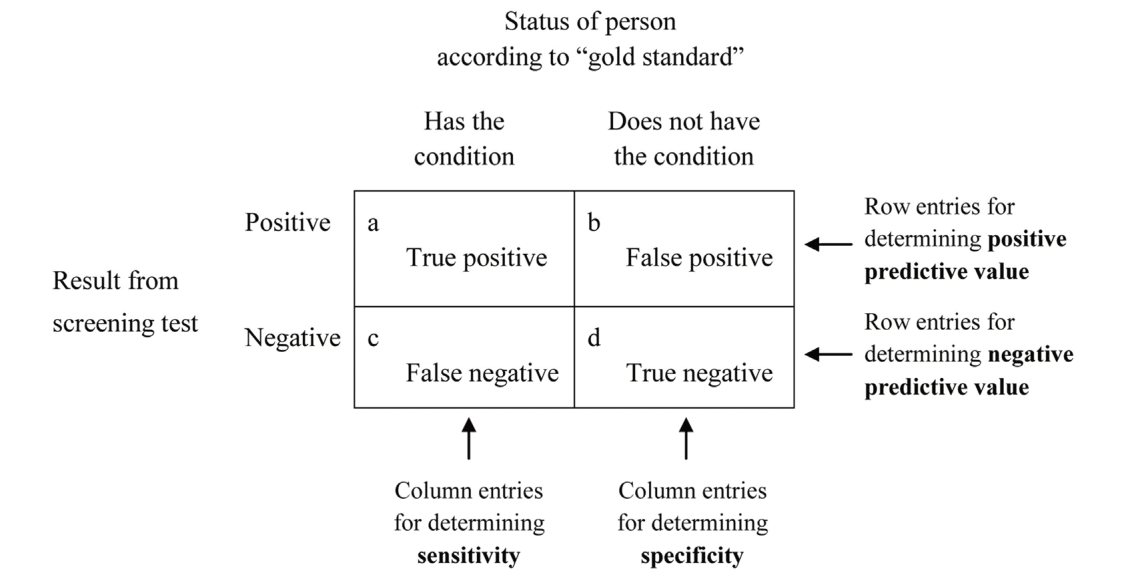
\includegraphics[width=1\textwidth]{images/2.literature_review/sensitivity_and_specificity.png}
    \captionof{figure}{Diagram demonstrating the basis for deriving sensitivity, specificity, and positive and negative predictive values\textsuperscript{1}}
    \label{fig:sensitivity_and_specificity}
\end{center}

\bigskip
        The sensitivity of a test refers to its ability to accurately detect true positives, meaning it correctly identifies all individuals who have a condition. That means that sensitivity is based solely on the cells labeled \textbf{a} and \textbf{c} in Figure \ref{fig:sensitivity_and_specificity}.\\
        Contrariwise, the specificity of a test measures its ability to accurately detect true negatives, meaning it correctly identifies individuals who do not have a condition. That means that specificity is based on the cells labeled \textbf{b} and \textbf{d} in Figure \ref{fig:sensitivity_and_specificity}.

\end{tcolorbox}

\footnotetext[1]{From \textit{Sensitivity, Specificity, and Predictive Values: Foundations, Pliabilities, and Pitfalls in Research and Practice} by R. Treevethan, 2017, Front in Public Health, 5, p. 307. Creative Commons Attribution License }

The research conducted by \citeA{navarro_colorectal_2017} demonstrates the extensive adoption of CRC screening strategies globally, encompassing most European countries, Canada, specific regions in North and South America, Asia, and Oceania. These initiatives typically employ either the FIT or fecal occult blood test (FOBT) in conjunction with colonoscopies to facilitate early detection of CRC within their respective populations. The study highlights varying participation rates, with notable examples such as the Netherlands boasting a 68.2\% participation rate, providing valuable insights into successful approaches. On the other hand, instances like Canada, with participation rates as low as 16\%, underscore potential practices to be avoided.

\section{Briging the Gap: Operations Research and Process Mining}

Operations Management, for many years, has developed tools for process analysis, which are commonly found in any reference of the discipline \cite{rama_murthy_operations_2007}. However, in recent times, the digitization of many processes has made a large amount of data available regarding the processes and the flows of activities within them. The analysis of this data using sophisticated tools, such as those derived from Machine Learning topics, taking into account the underlying processes, has led to the methodology called Process Mining, which has been very successful in the analysis and improvement of complex processes \cite{van_der_aalst_process_2004}.

\section{Process Mining}

Process Mining, as a methodological approach, has gained prominence in various industries for its capability to extract valuable insights from event data. For example, it has been used in education to help predict the success of students in massive online courses with high accuracy \cite{umer_predicting_2017}, and in product design to enhance medical machines that require operator interaction \cite{reindler_siemens_2020}.

In the healthcare sector, where process complexity often impedes efficient care delivery, there are numerous instances where process mining holds the potential to uncover hidden patterns, identify bottlenecks, and enhance overall service quality \cite{rojas_process_2016}. Various authors advocate that this tool allows for modeling processes and studying them from different perspectives, including visual representations, activity durations, time between activities, variability, expected behavior versus actual behavior, and many others \cite{bozkaya_process_2009}.

When applied to CRC care, Process Mining serves as a lens through which the complexities of detection, confirmation, categorization, and treatment processes can be systematically analyzed.

\section{Simulation}

Simulation holds significant importance within in the realm of Operations Research \cite{de_paula_ferreira_simulation_2020}, serving as a powerful tool for analyzing complex systems and making informed decisions. In Operations Research, Simulation enables researchers and practitioners to model intricate processes, test various scenarios, and evaluate the impact of different strategies without the need for real-world experimentation. According to Dr. Nelson in \cite{fu_simulation_2014}, Simulation is typically used for three reasons: feasibility (“We have a plan, will it work?”); sensitivity (“We’re not really sure about everything, so how much does it matter?”); and optimization (“What are the good options and how good are they?”). Simulation Optimization is a well known topic in the Simulation community, addressing the problem of designing complex systems by finding the best settings of design variables.

Similarly, in healthcare, Simulation plays a crucial role in improving the delivery of care, enhancing patient outcomes, and optimizing resource allocation \cite{jun_application_1999}. Healthcare systems are inherently complex, involving a multitude of interconnected factors such as patient flow, resource utilization, staffing levels, and treatment protocols. Simulation in healthcare serves primarily four purposes: health and care systems operation (HCSO), disease progression modeling (DPM), screening modeling (SM), and health behavior modeling (HBM), with the most prevalent being HCSO, followed by DPM, SM, and HBM, respectively \cite{zhang_application_2018}. From predicting patient wait times in emergency departments to optimizing operating room schedules and evaluating the efficacy of new treatment protocols, Simulation offers invaluable insights that can inform decision-making, improve efficiency, and ultimately enhance patient care.

Screening simulations are essential tools for evaluating the potential implementation of screening programs, assessing their impact on prognosis, cost-effectiveness, and implementation feasibility. These simulations find applications in various healthcare areas, including the detection of diseases like diabetic retinopathy \cite{davies_evaluation_2002} and numerous types of cancers \cite{bespalov_cancer_2021}.

Prior to the twenty-first century, computer simulations were not seen as providing evidence definitive enough to shape screening recommendations \cite{phillips_screening_2020}. A major turning point for the CRC screening simulations came when three independent simulation models were developed for CRC: the MIcrosimulation SCreening Analysis Colorectal Cancer Model (MISCAN-Colon)\cite{loeve_miscan-colon_1999}, the Simulation Model of Colorectal Cancer (SimCRC)\cite{knudsen_rescreening_2012}, and the Colorectal Cancer Simulated Population model for Incidence and Natural history (CRC-SPIN)\cite{rutter_bayesian_2009}. The MISCAN-Colon model, introduced in 1999, has served as a foundational framework for numerous subsequent models developed in the following years \cite{smith_simulation_2020}.

\chapter[Methodology]{Methodology}
\label{chapter:methodology}

This chapter aims to offer a thorough examination of the methodology applied in the investigative phase of this thesis. Before exploring the two main components outlined within, an introductory section elucidates the functions of Process Mining, its tools, and the methodology to be utilized in the analysis. The first phase involves systematically revealing the colorectal cancer (CRC) care process at the SMPHS through data collection and preprocessing. Following this, the second component involves identifying and analyzing the current situation within the existing scenario using the Process Mining output, as well as proposing potential improvements.

\section{Process Minning}

Process Mining (PM) utilizes algorithms and techniques to analyze event data and automatically extract process models. It is regarded as an interdisciplinary field that intersects various disciplines encompassed within the domains of data science and process science. Data mining principles are applied to uncover patterns, trends, and anomalies within process data.

\begin{figure}[H]
    \centering
    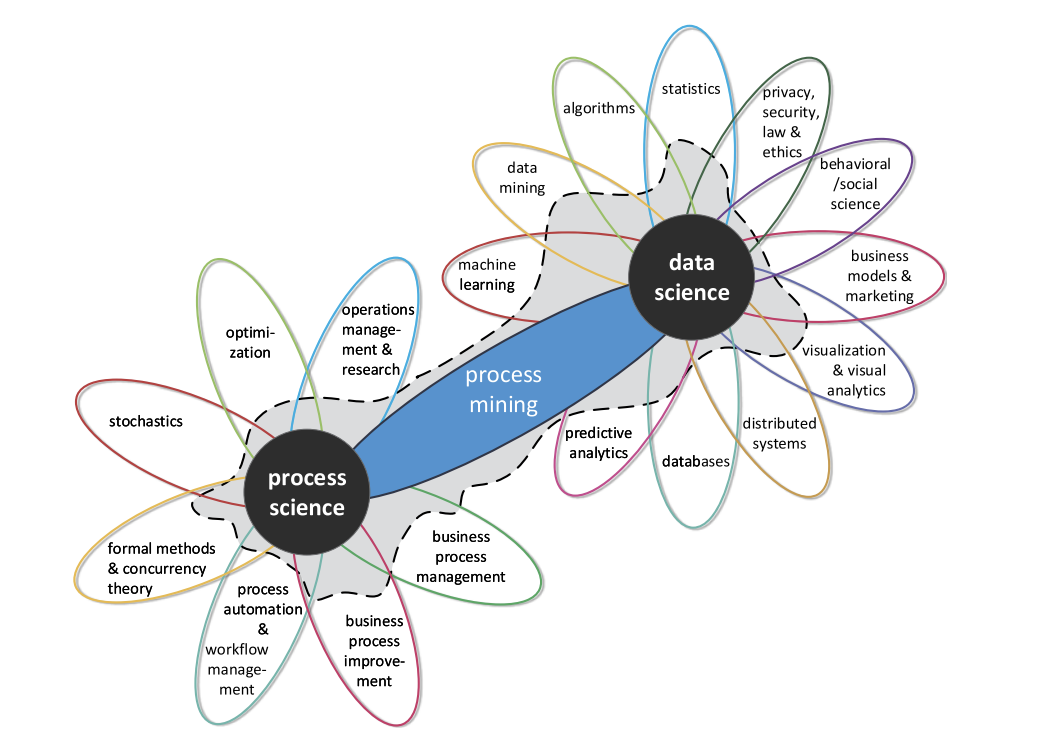
\includegraphics[width=1\textwidth]{images/3.methodology/process_mining.png}
    \caption[Process Mining as an interdisciplinary Discipline]{Process Mining as an interdisciplinary Discipline \textsuperscript{1}}
    \label{fig:process_mining}
\end{figure}

\addtocounter{footnote}{1}
\footnotetext[\value{footnote}]{From \textit{Process Mining}(p.18), by Wil van der Aalst, 2016, Berlin, Heidelberg: Springer Berlin Heidelberg. Copyright [2016] by Springer Berlin Heidelberg.}
As depicted in Figure \ref{fig:process_mining}, process mining intersects with domains in data science, including statistics, databases, computational intelligence, data mining, and visual analytics. Simultaneously, it intersects with domains in process science, such as business process management, optimization, stochastics, process automation and workflow management, and operations management and research. Process mining serves as a bridge between data and process science \cite{van_der_aalst_process_2016}.

\subsection*{PM Methodology and Techniques}

A standard methodology for such projects was established by \citeA{van_eck_pm2_2015}, known as the Process Mining Project Methodology.

\begin{figure}[H]
    \centering
    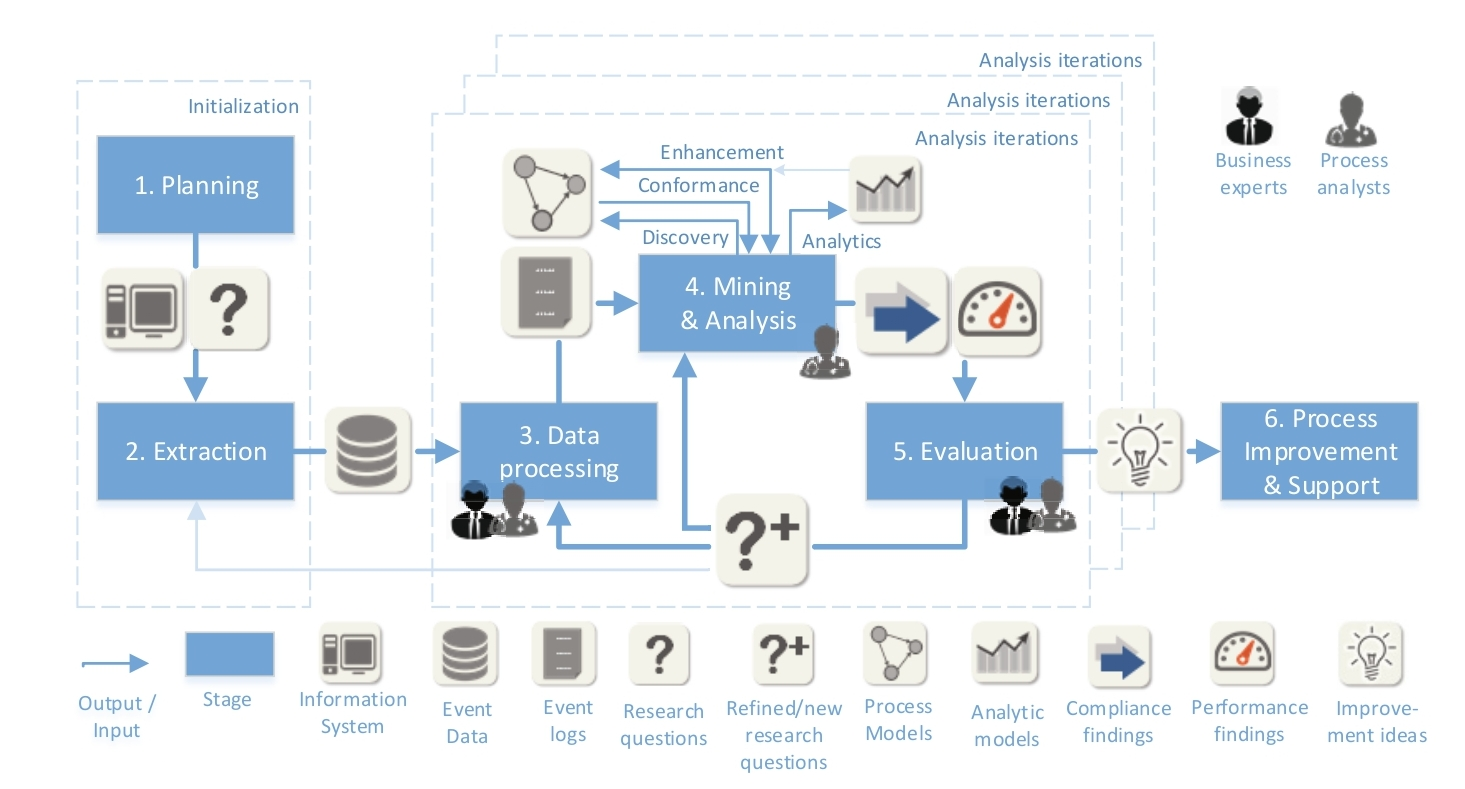
\includegraphics[width=1\textwidth]{images/3.methodology/process_mining_methodology.jpg}
    \caption[Overview of the Process Mining Project Methodology]{Overview of the Process Mining Project Methodology \textsuperscript{1}}
    \label{fig:process_mining_methodology}
\end{figure}

\footnotetext[\value{footnote}]{From \textit{PM\textsuperscript{2}: A Process Mining Project Methodology}(p.299), by van Eck et al., 2015, Cham, Springer International Publishing. Copyright [2015] by Springer International Publishing.}

Each stage depicted in Figure \ref{fig:process_mining_methodology} is carefully described by \citeA{van_eck_pm2_2015} in their publication. Here is an overview of each stage as described by them:

\begin{quote}
\textit{The first two stages of the methodology are (1) planning and (2) extraction, during which initial research questions are defined and event data are extracted. After the first two stages, one or more analysis iterations are performed, possibly in parallel. In general, each analysis iteration executes the following stages one or more times: (3) data processing, (4) mining \& analysis, and (5) evaluation. An analysis iteration focusses on answering a specific research question by applying process mining related activities and evaluating the discovered process models and other findings. Such an iteration may take anywhere from minutes to days to complete, mainly depending on the complexity of the mining \& analysis. If the findings are satisfactory then they can be used for (6) process improvement \& support.}
\end{quote}

\begin{figure}[H]
    \centering
    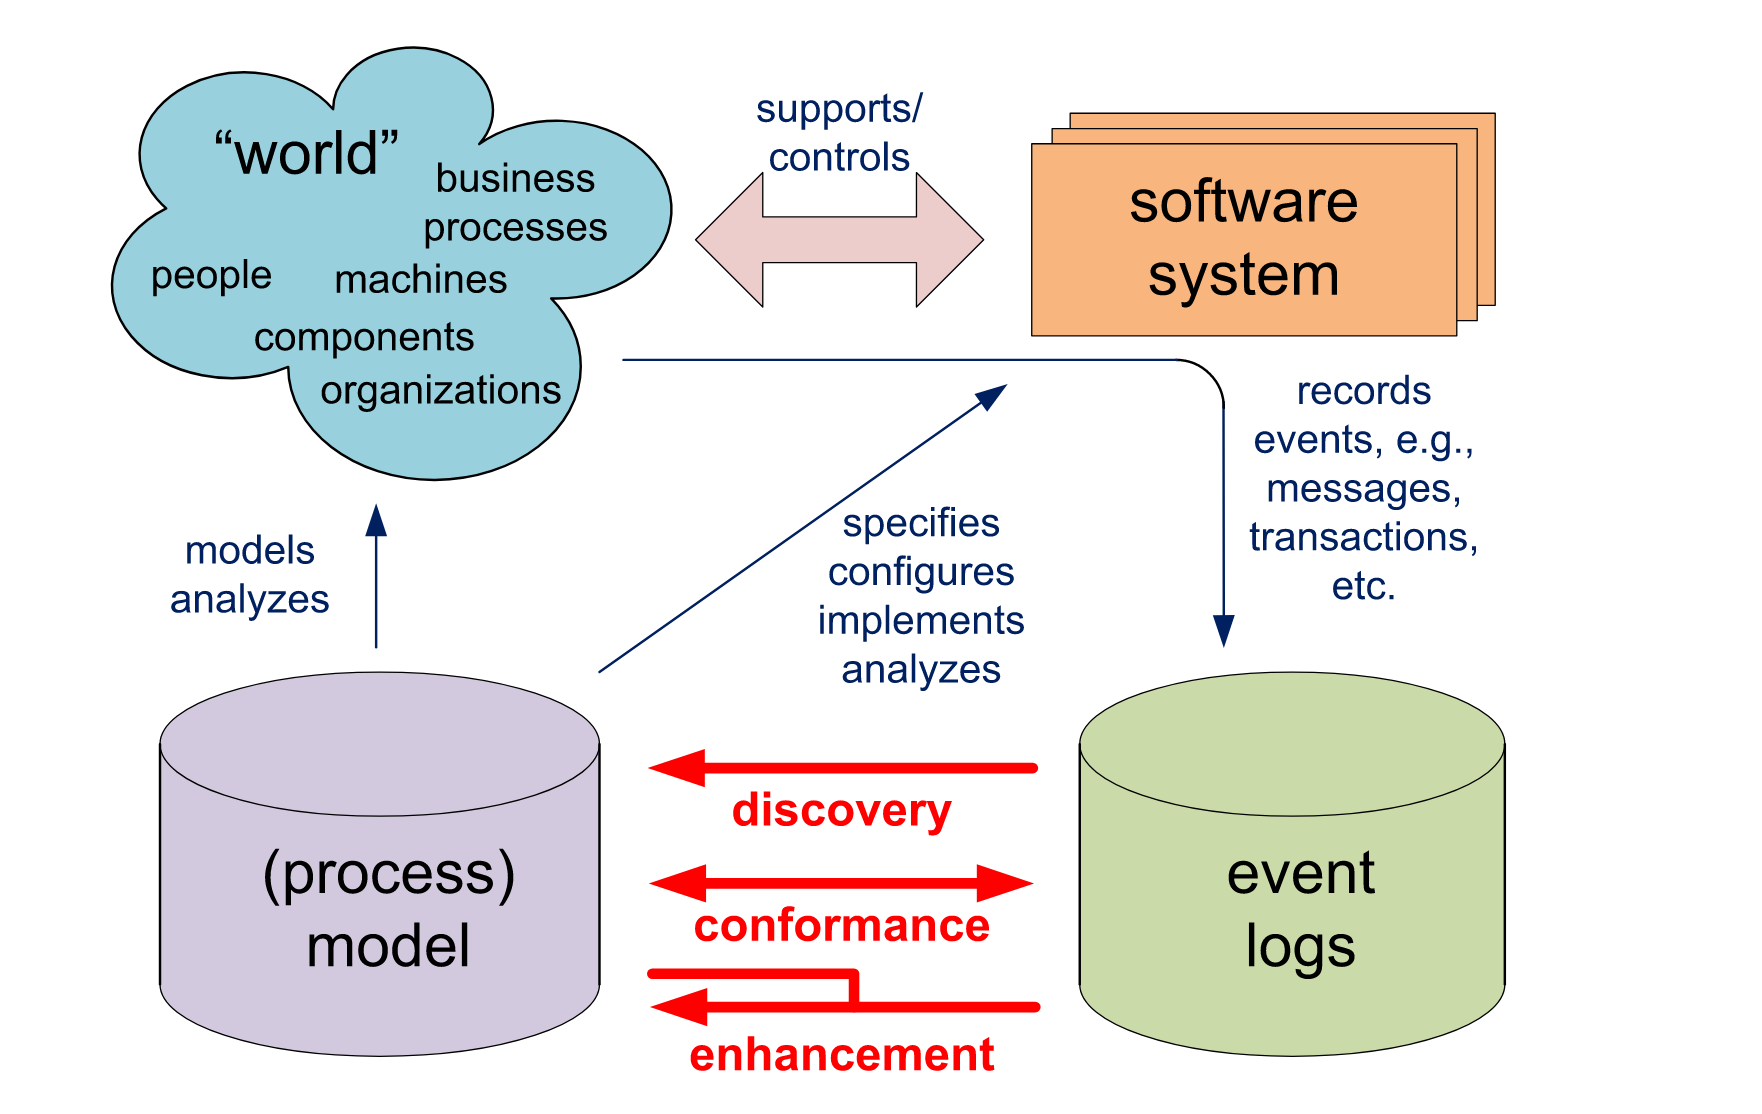
\includegraphics[width=1\textwidth]{images/3.methodology/process_mining_techniques.png}
    \caption[Process Mining Techniques]{Process Mining Techniques \textsuperscript{1}}
    \label{fig:process_mining_techniques}
\end{figure}

\footnotetext[\value{footnote}]{From \textit{Process Mining}(p.32), by Wil van der Aalst, 2016, Berlin, Heidelberg: Springer Berlin Heidelberg. Copyright [2016] by Springer Berlin Heidelberg.}

As depicted in Figure \ref{fig:process_mining_techniques}, the core techniques in PM consist of Process Discovery, Conformance Checking, and Process Enhancement. Process Discovery involves extracting process models from a log, while Conformance Checking examines deviations by comparing the model and log. Process Enhancement extends or refines existing models using a log. In this study, our focus was exclusively on Process Discovery. This decision was made by the absence of a rigorous model depicting the Stage or Benefits process, rendering Conformance Checking pointless. Additionally, as process enhancements were guided by professional recommendations rather than the refinement of an existing model, the Process Enhancement technique was also considered impractical.

\subsection*{Specialized Methodology for Exploring CRC Care Processes}

While standard methodologies and techniques provide a broad understanding of typical PM projects, this study employed a specific approach tailored to its objectives. The primary aim of PM in this study was to explore the CRC care process through Process Discovery. To achieve this, we utilized a specialized methodology developed by \citeA{vathy-fogarassy_multi-level_2022}, known as the Process Mining Methodology for Exploring Disease-specific Care Processes (MEDCP).

This methodology is designed to address the intricacies of exploring disease-specific care processes by working at different levels of abstraction. It involves preprocessing the data to group detailed activities into higher event groups, allowing researchers to view activities from a simplified perspective without ignoring less frequently traveled pathways.

\begin{figure}[H]
    \centering
    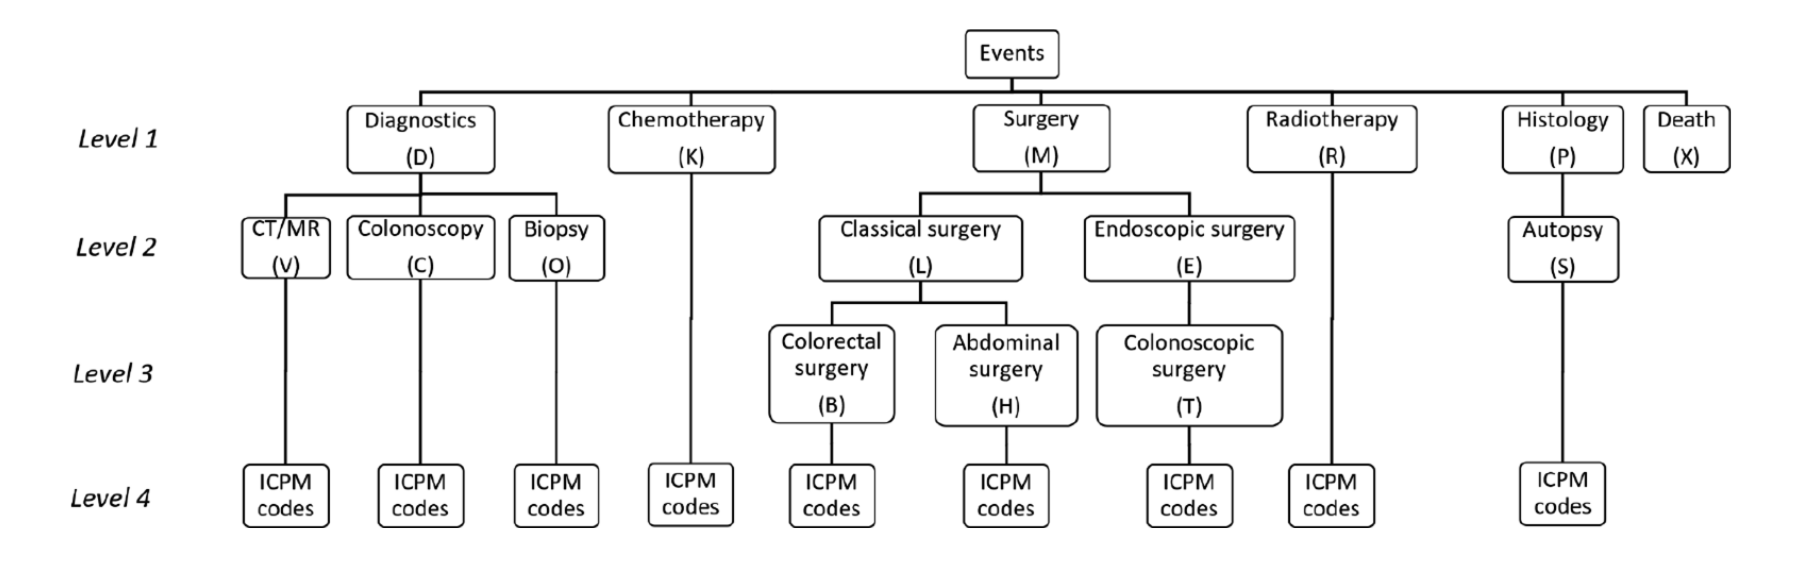
\includegraphics[width=1\textwidth]{images/3.methodology/MEDDCP_CRC_case.png}
    \caption[CRC Multi-level Abstraction]{CRC Multi-level Abstraction\textsuperscript{1}}
    \label{fig:crc_case}
\end{figure}

\footnotetext[\value{footnote}]{From \textit{Multi-level process mining methodology for exploring disease-specific care processes}(p.8), by Vathy-Fogarassy, 2022, Hungary, Jorunal of Biomedical Informatics Copyright [2022] by Journal of Biomedical Informatics.}

As depicted in Figure \ref{fig:crc_case}, for the CRC case detailed by \citeA{vathy-fogarassy_multi-level_2022} in their publication, the methodology organizes interventions into four levels: detailed procedures into Level 4, surgeries into Level 3, main procedures into Level 2, and main stages of CRC care into Level 1.

This approach proved invaluable, particularly in the selection and preprocessing of data, as it addressed many of the challenges encountered by the researcher. Furthermore, the separation of benefits and stages within the datasets facilitated multi-level abstraction, providing a comprehensive view of the CRC care process in two levels.

\subsection*{The Software of Choice}

For this study, Disco (\href{www.fluxicon.com}{www.fluxicon.com}) was selected as the software of choice from a range of Process Mining tools, including ProM (\href{www.promtools.org}{www.promtools.org}) and Celonis (\href{www.celonis.com}{www.celonis.com}), all of which the researcher is familiar with. Disco proved to be the optimal solution due to its user-friendly interface and robust functionality. Its intuitive design facilitated seamless data import and visualization, simplifying the exploration of complex process models. Additionally, Disco's comprehensive range of analysis features enabled thorough examination of the CRC care pathway within the SMPHS. Its efficient handling of large datasets proved instrumental in managing the extensive healthcare data required for this investigation. Overall, Disco's combination of accessibility, versatility, and performance made it the ideal choice for conducting Process Mining analysis in this research endeavor.

Next, we will outline the key features of the Disco software.

\begin{figure}[H]
    \centering
    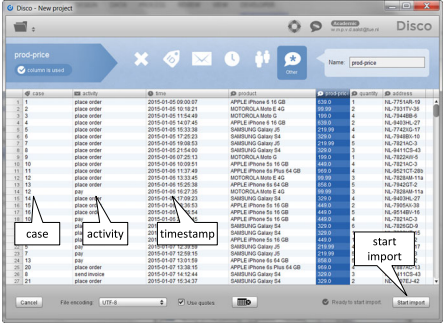
\includegraphics[width=1\textwidth]{images/3.methodology/disco_import.png}
    \caption{Importing a File in Disco}
    \label{fig:disco_importing_file}
\end{figure}

As depicted in Figure \ref{fig:disco_importing_file}, the process of importing files into the system is straightforward. Simply choose the file and indicate which columns will serve as the Case ID, Activity, and Timestamp for both the start and end of each activity. After selecting to start the import, a process map will be displayed.

\begin{figure}[H]
    \centering
    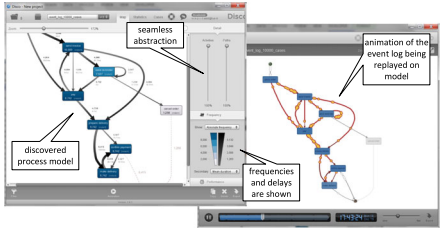
\includegraphics[width=1\textwidth]{images/3.methodology/disco_features.png}
    \caption{Main Disco Features}
    \label{fig:disco_features}
\end{figure}

As depicted in the left image of Figure \ref{fig:disco_features}, the software interface features a process map displayed on the left side. The seamless abstraction panel, positioned at the top right, enables users to adjust the visibility of Activities and Paths within the discovered process model or process map. Additionally, the Frequency and Performance panel located in the bottom right corner of the screen enables users to switch between these two modes, although the Performance mode will not be utilized in this study. Furthermore, users can utilize the Animation panel at the bottom to visualize how individuals behave within the process map, as depicted in the right image of Figure \ref{fig:disco_features}.

\subsection*{Illustrative Example}

When initiating a new project, the initial process map often becomes overwhelming when all activities and paths are included, resulting in what is commonly referred to as "spaghetti maps" due to their complex and tangled appearance.

\begin{figure}[H]
    \centering
    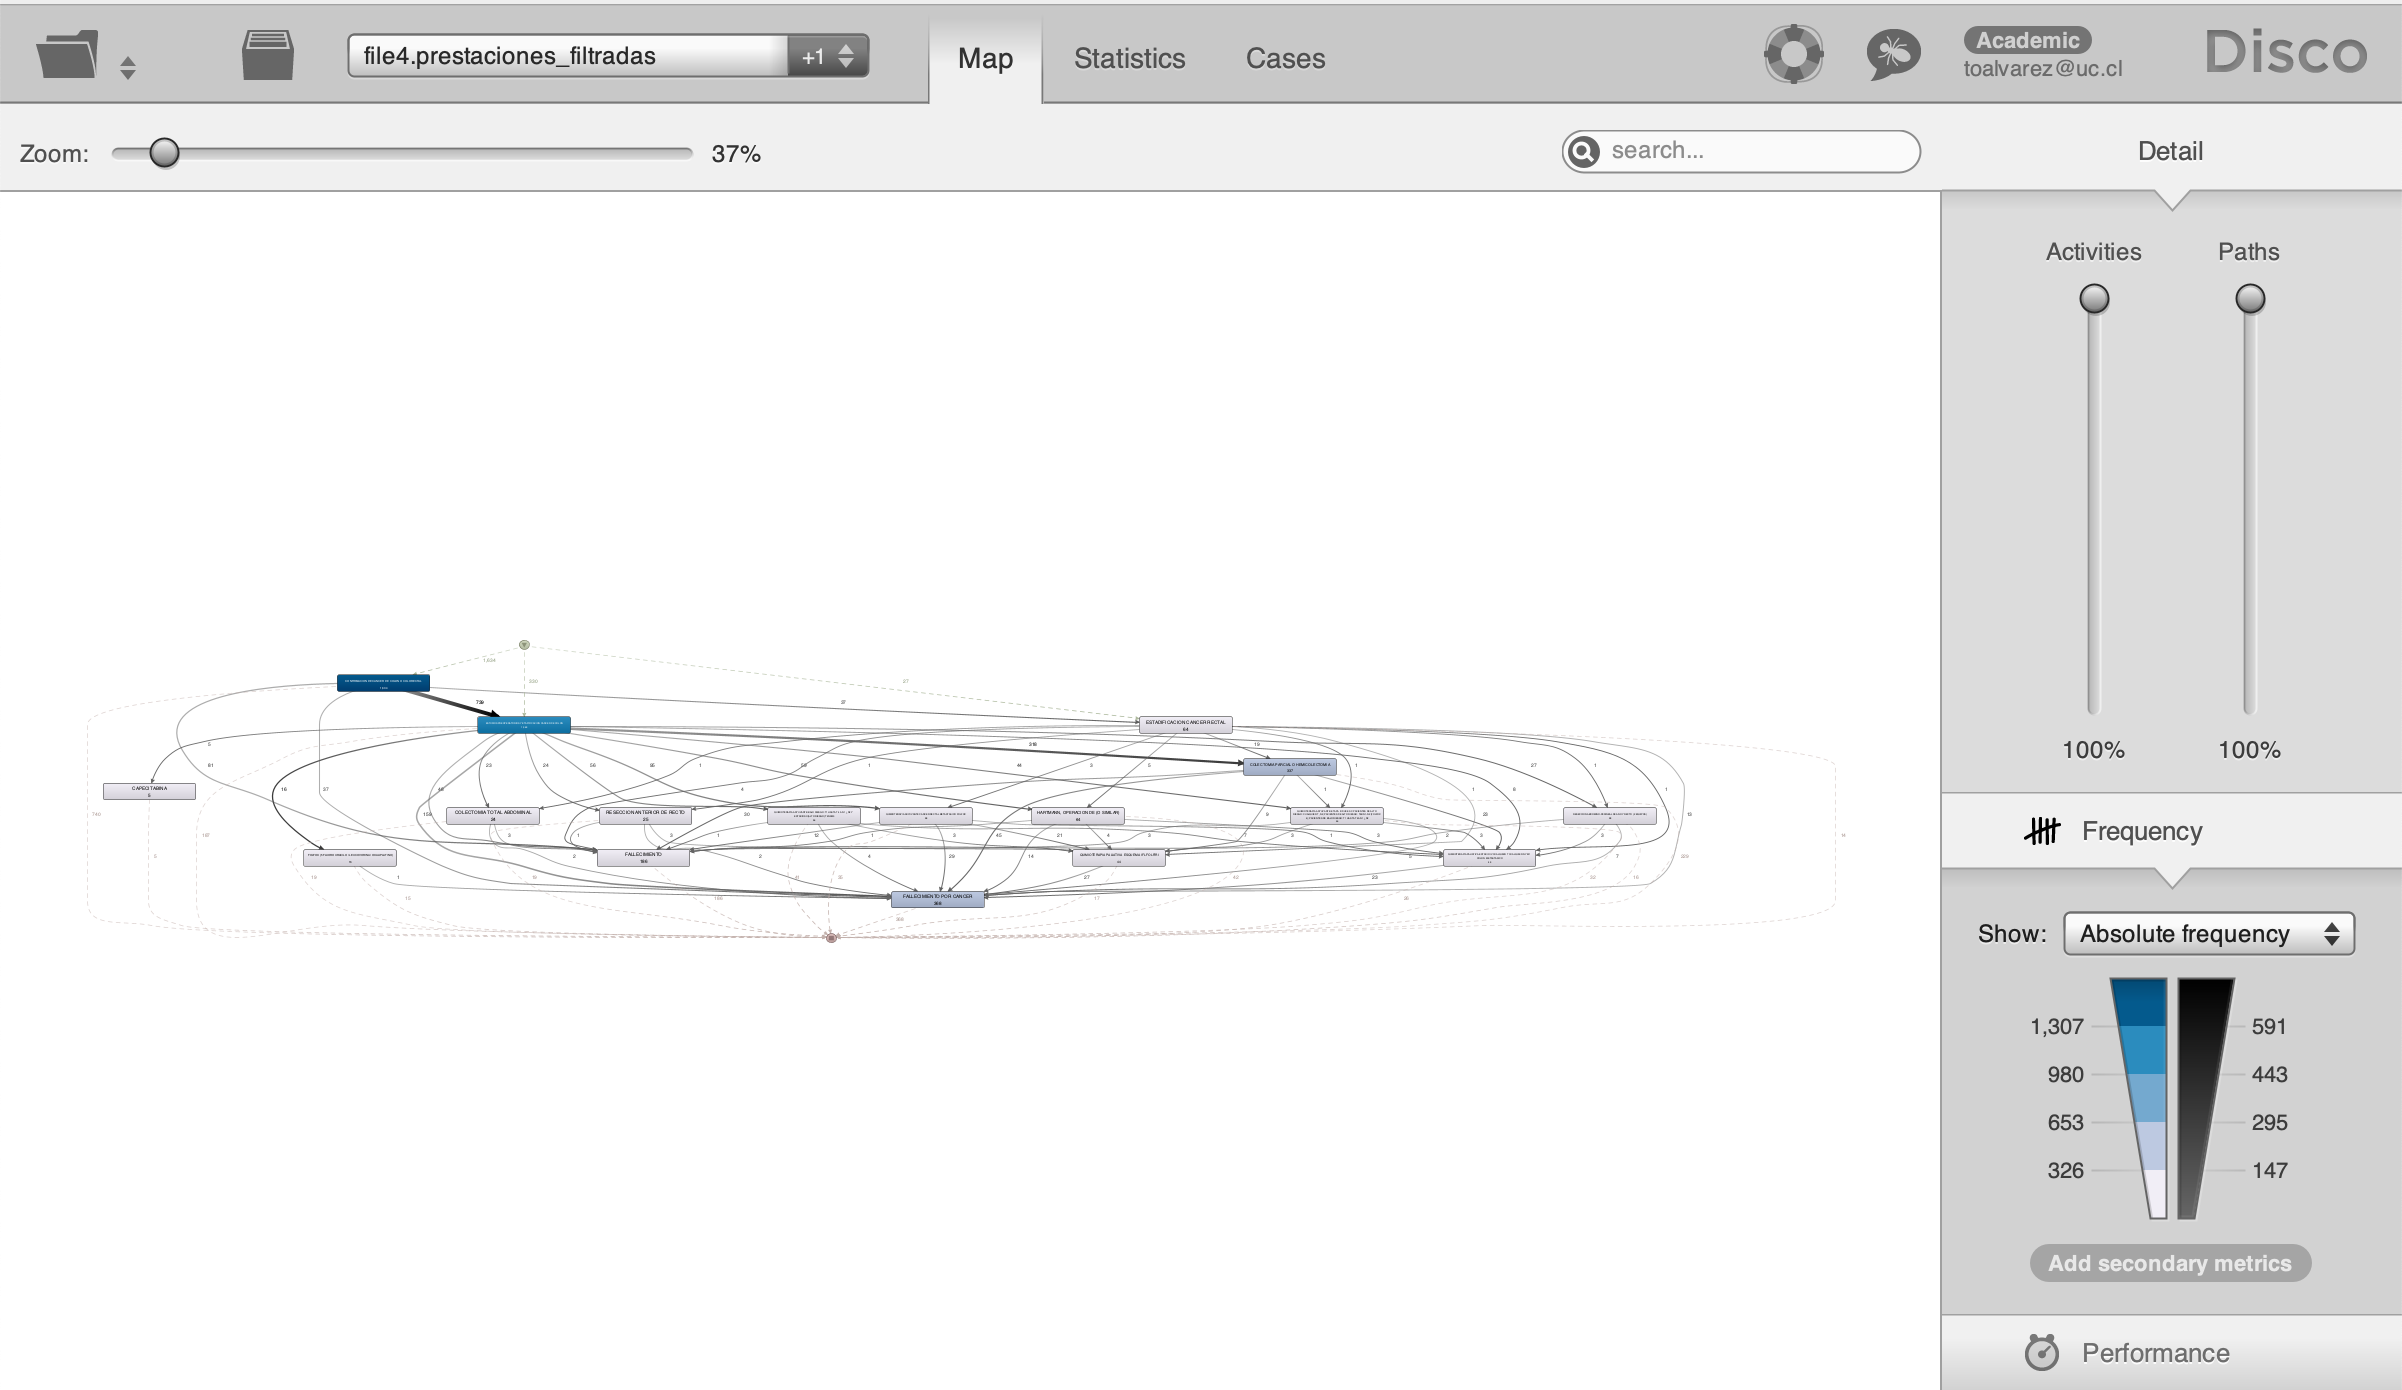
\includegraphics[width=1\textwidth]{images/3.methodology/disco_example_1.png}
    \caption{Disco Benefits Example}
    \label{fig:disco_example_1}
\end{figure}

For instance, Figure \ref{fig:disco_example_1} presents a spaghetti map depicting the Benefits process of CRC patients. To enhance readability, the number of paths has been reduced to approximately 20\% of the most common paths.

\begin{figure}[H]
    \centering
    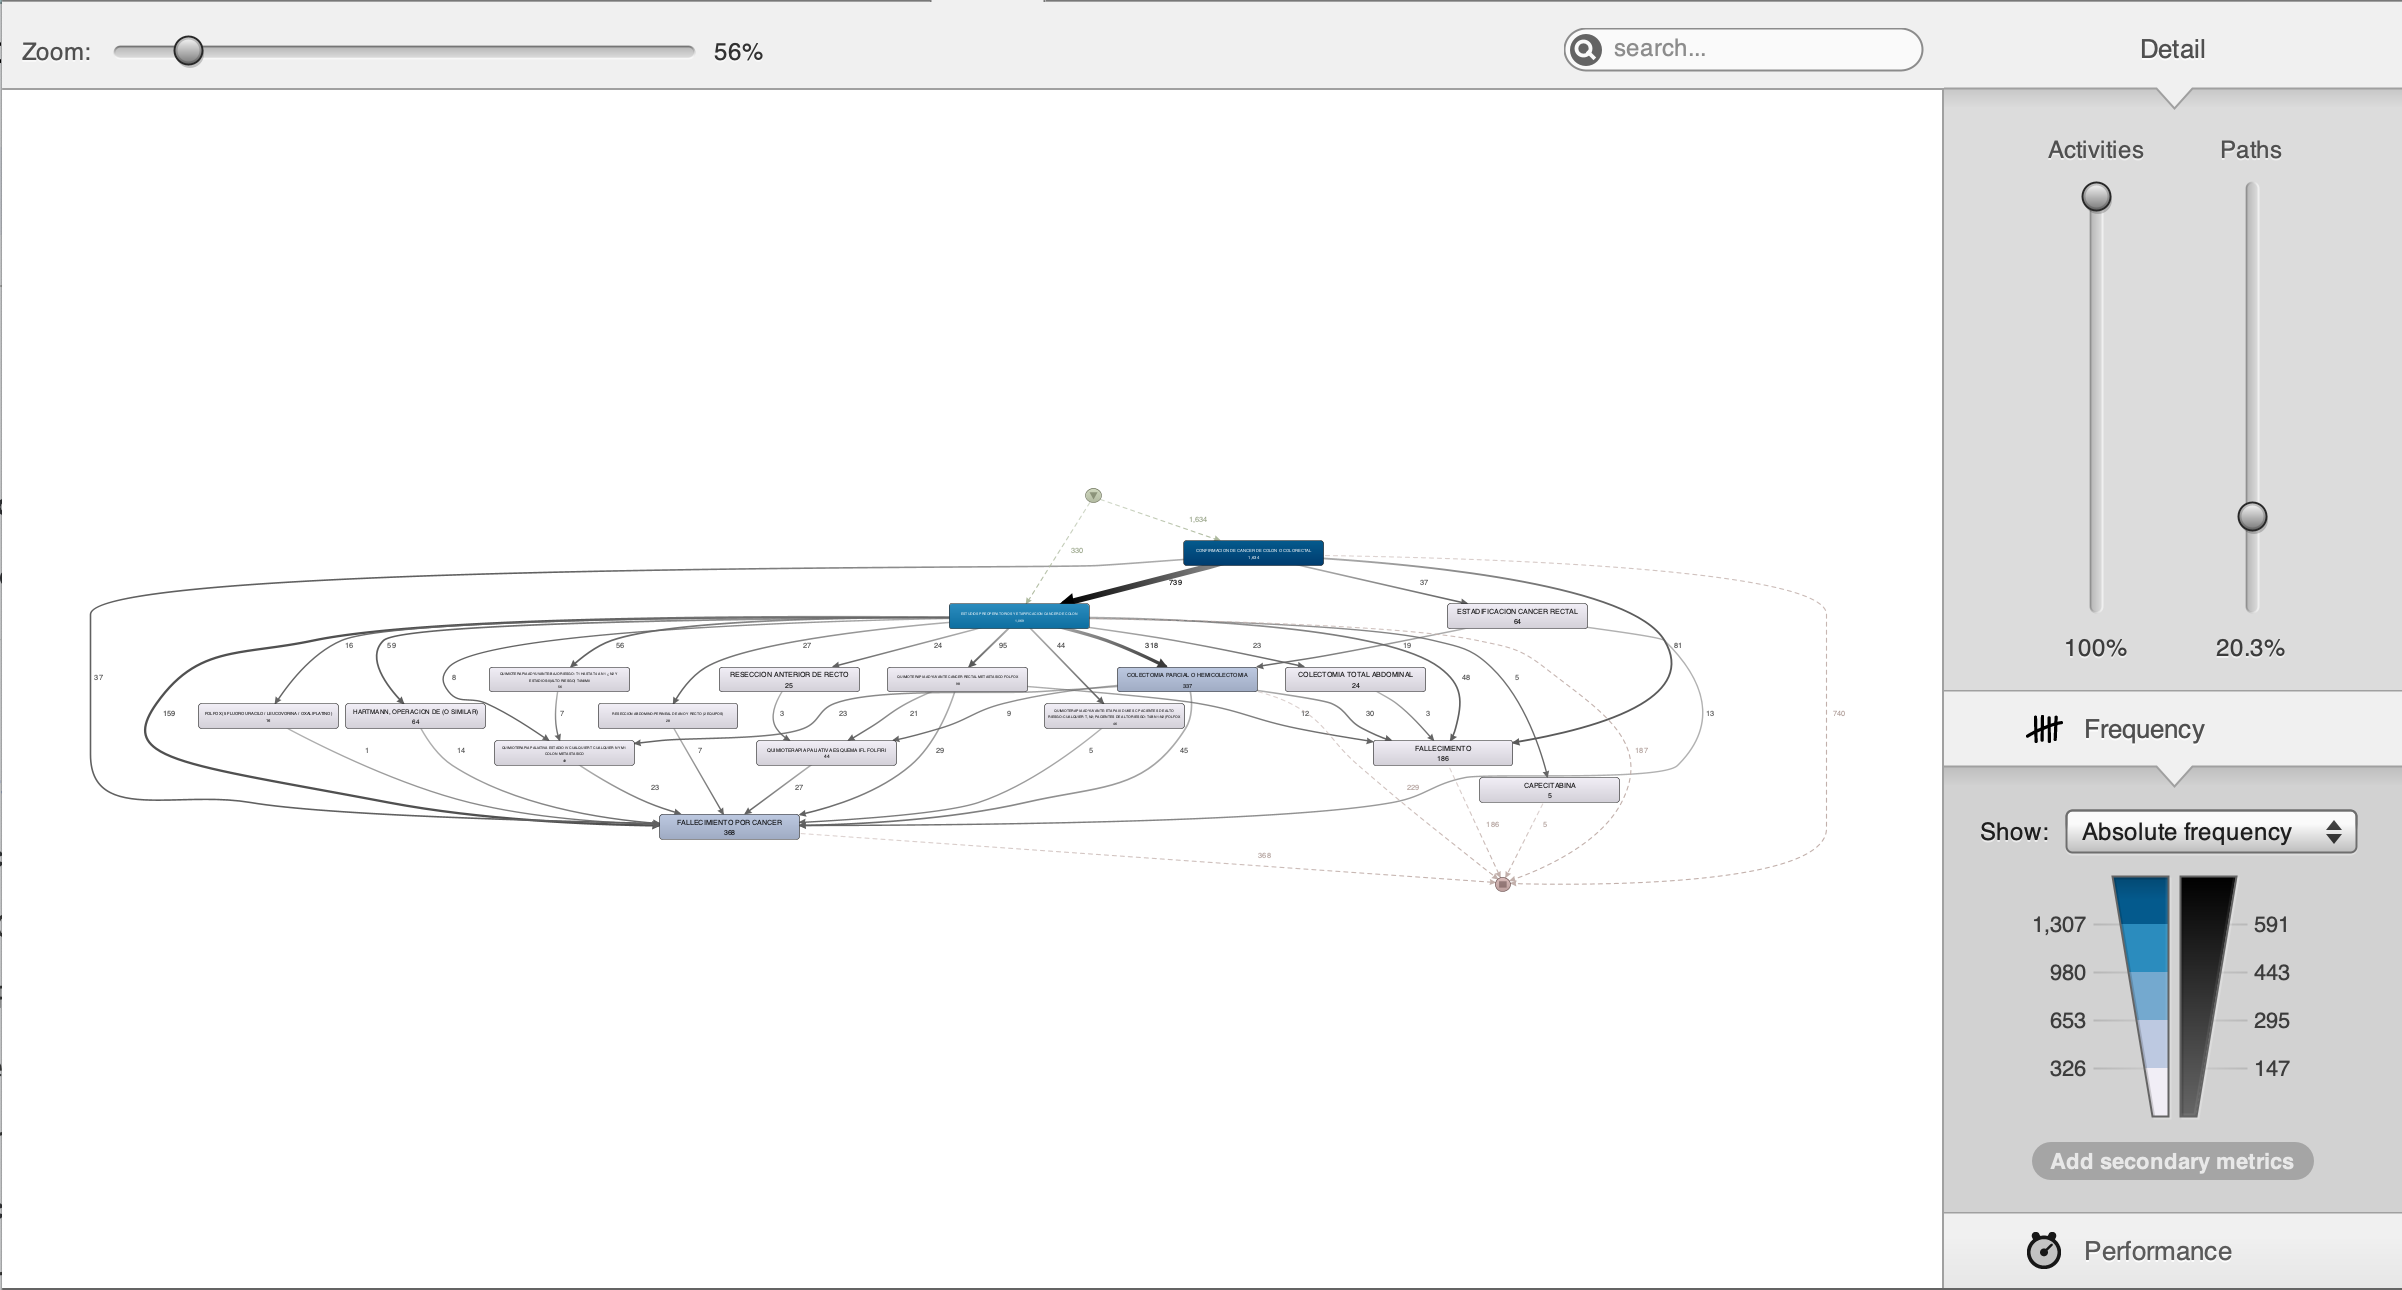
\includegraphics[width=1\textwidth]{images/3.methodology/disco_example_2.png}
    \caption{Disco Benefits Example Activities at 20\%}
    \label{fig:disco_example_2}
\end{figure}

Despite this adjustment, due to the multitude of activities involved, in Figure \ref{fig:disco_example_2} clarity remains a challenge. To address this, the number of activities will also be reduced to around 20\% of the most common activities.

\begin{figure}[H]
    \centering
    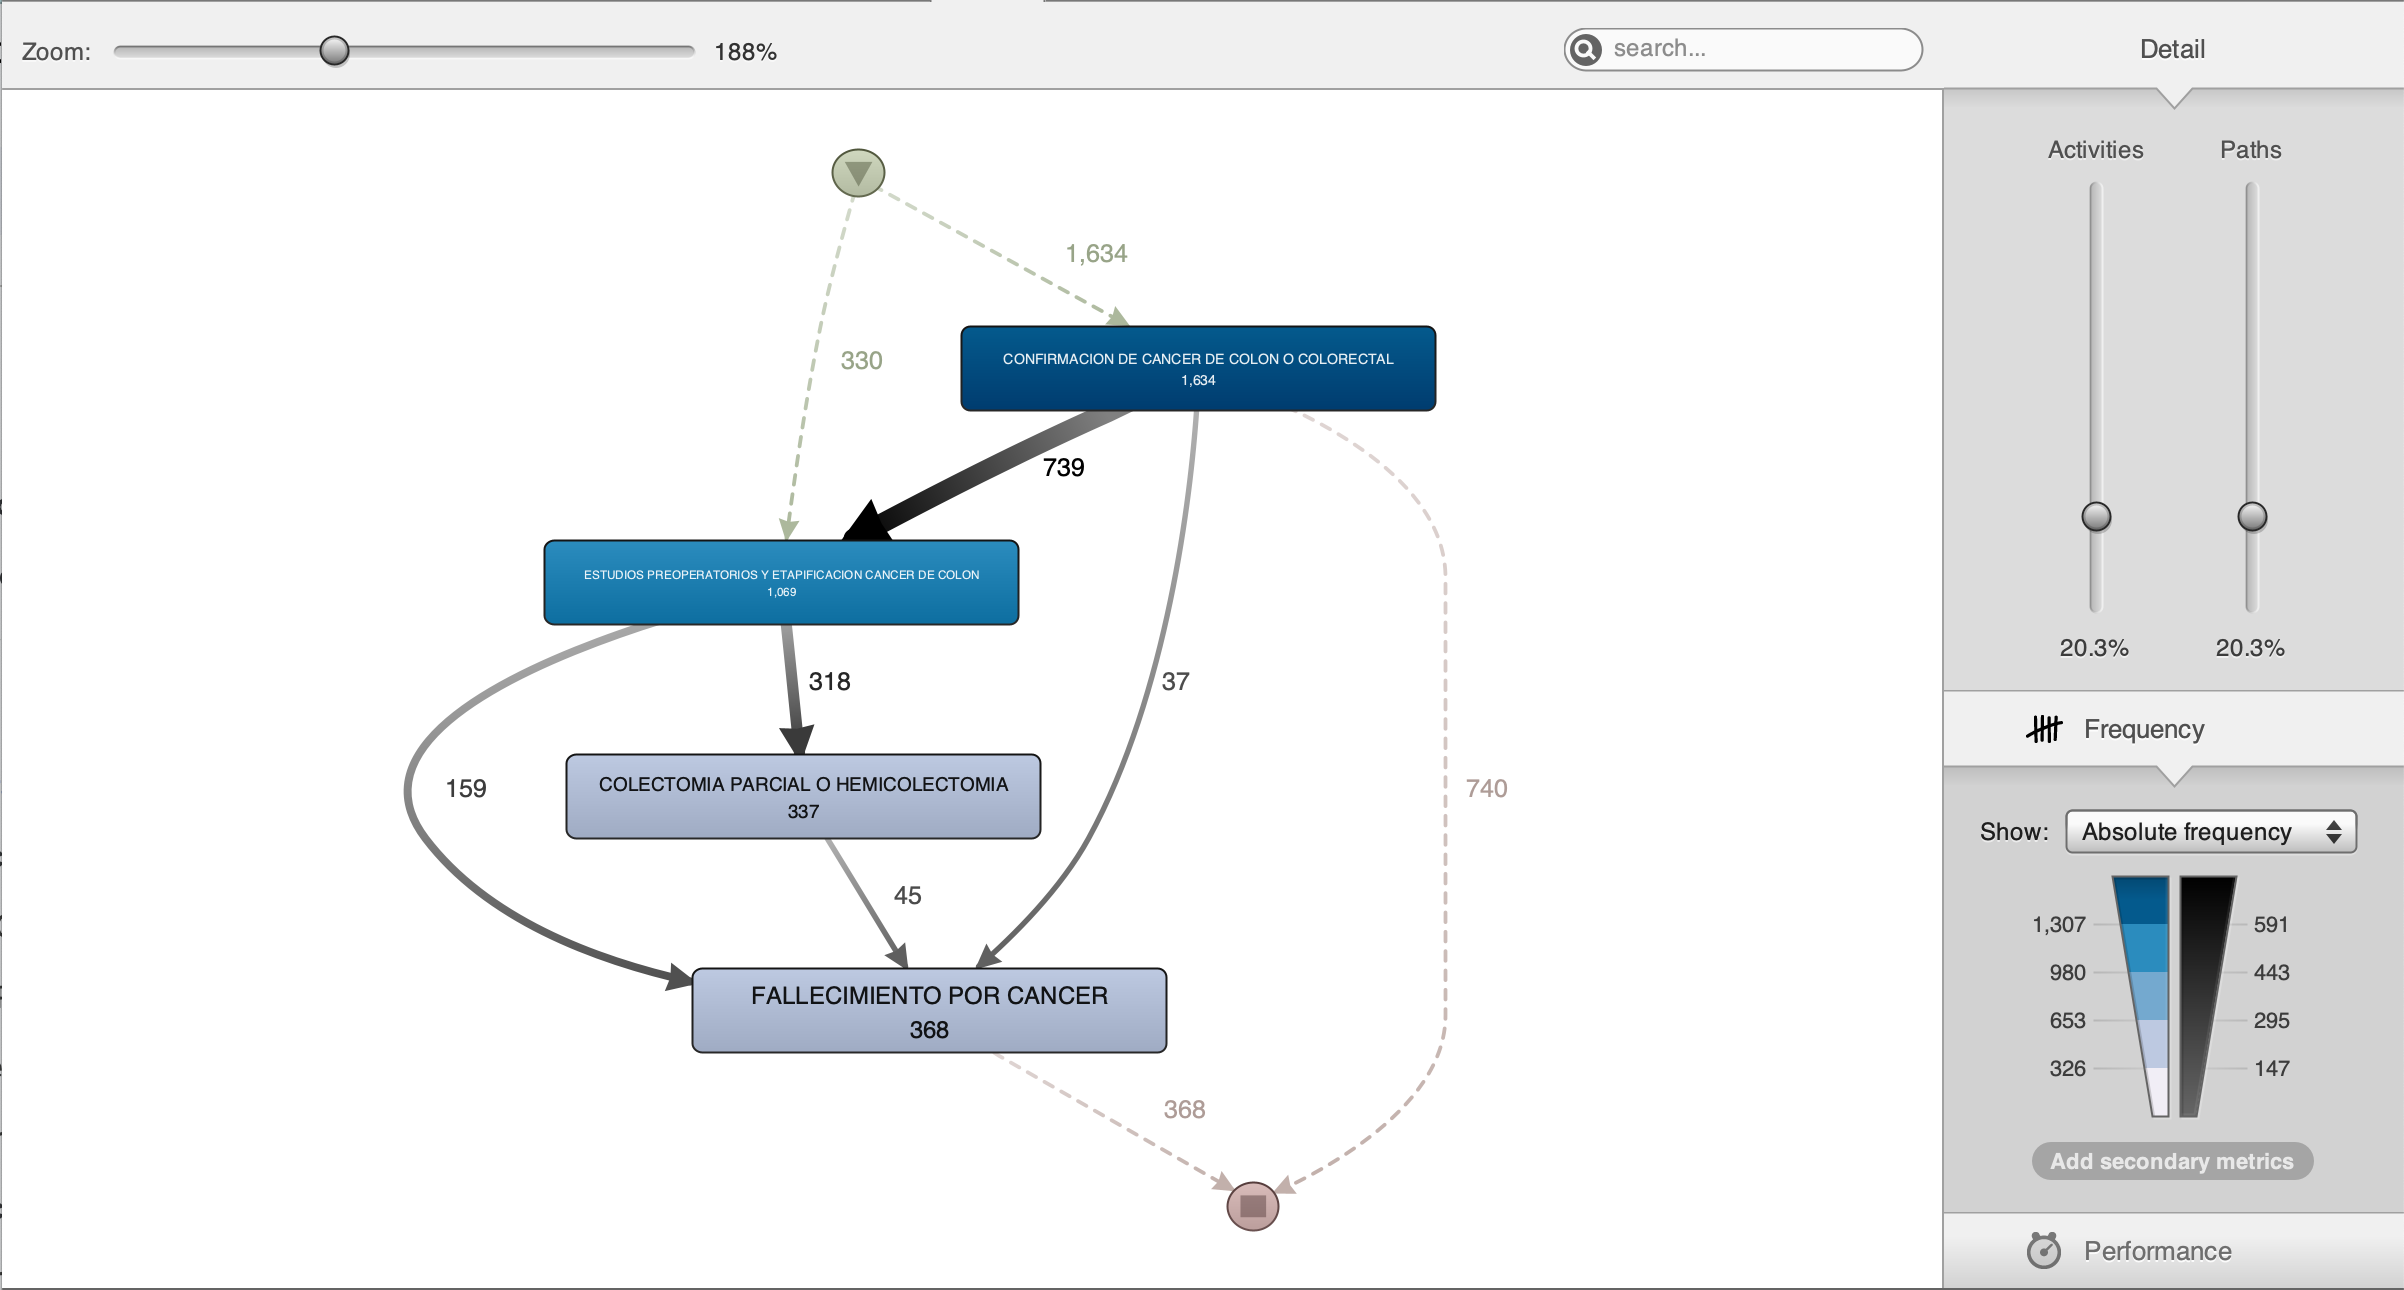
\includegraphics[width=1\textwidth]{images/3.methodology/disco_example_3.png}
    \caption{Disco Benefits Example Activities and Paths at 20\%}
    \label{fig:disco_example_3}
\end{figure}

In the updated Figure \ref{fig:disco_example_3}, we observe a significantly more legible process map. The dominant activity, "CONFIRMACION DE CANCER DE COLON O COLORECTAL" (Confirmation of CRC), appears prominently, occurring 1634 times. The shading of the activities indicates their frequency, with darker color representing higher occurrence. Likewise, the thickness of the arrows representing transitions between activities reflects their frequency. Additionally, the Frequency panel can be adjusted to provide insights into the average duration of each activity transition.

\begin{figure}[H]
    \centering
    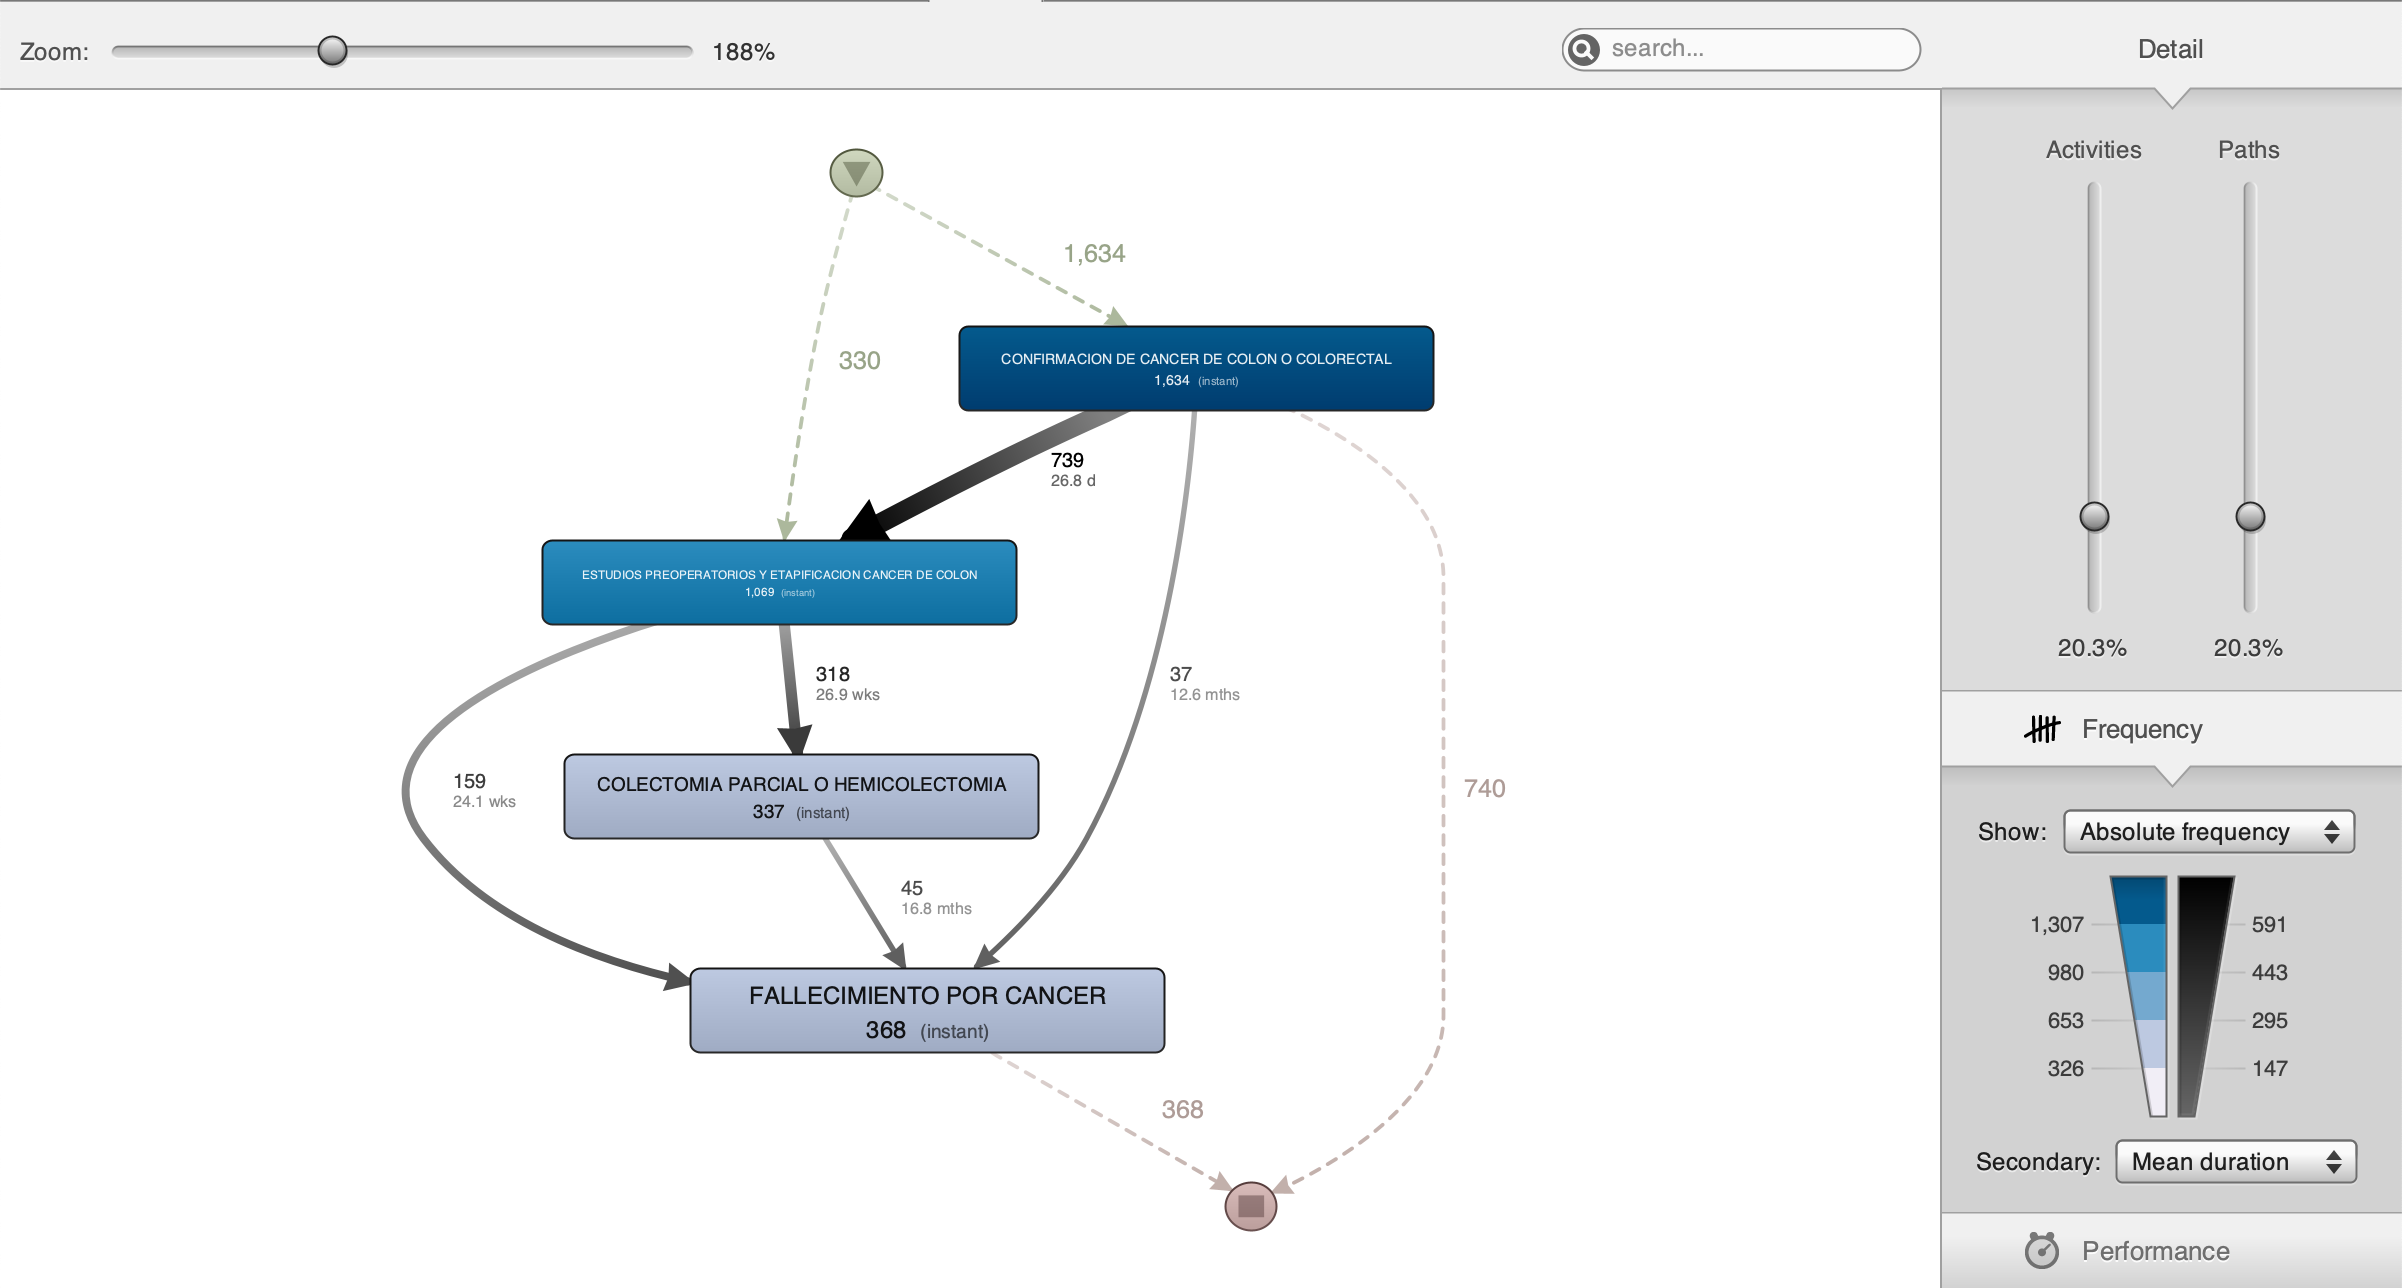
\includegraphics[width=1\textwidth]{images/3.methodology/disco_example_4.png}
    \caption{Disco Benefits Example with Mean Duration}
    \label{fig:disco_example_4}
\end{figure}

Further analysis, as depicted in figure \ref{fig:disco_example_4}, reveals the average transition time between activities. For instance, between "CONFIRMACION DE CANCER DE COLON O COLORECTAL" and "ESTUDIOS PREOPERATORIOS Y ETAPIFICACION CANCER DE COLON" (preoperative evaluation and CRC staging), 739 transitions occurred, with an average duration of 26.8 days. It's important to note that this calculation relies on the availability of timestamps marking the start and, ideally, the end of each activity. In cases where only one timestamp is available, indicating the activity's initiation, the duration is represented as "instant."

\section{Process Discovery}

The process discovery stage adopts the MEDCP methodology described by \citeA{vathy-fogarassy_multi-level_2022}. Initially, data is collected, followed by a meticulous cleaning process to construct event logs, a fundamental prerequisite for process mining analysis. Subsequently, the refined event logs are used to initiate process discovery through the process maps generated by the selected software. Furthermore, insights from the MND team are incorporated to deepen the understanding of the CRC care process. Lastly, performance metrics are introduced to offer additional insights for the process analysis.
\subsection*{Data Collection}

The data collected is primarily sourced from the comprehensive information cataloged by the SIGGES program. This government initiative, integral to monitoring benefits under the Explicit Guarantees in Health (GES) program, guarantees access to specific healthcare exams and treatments for a predetermined list of prevalent diseases. Two comprehensive datasets were provided by the MND team to support this research. 

\begin{figure}[H]
    \centering
    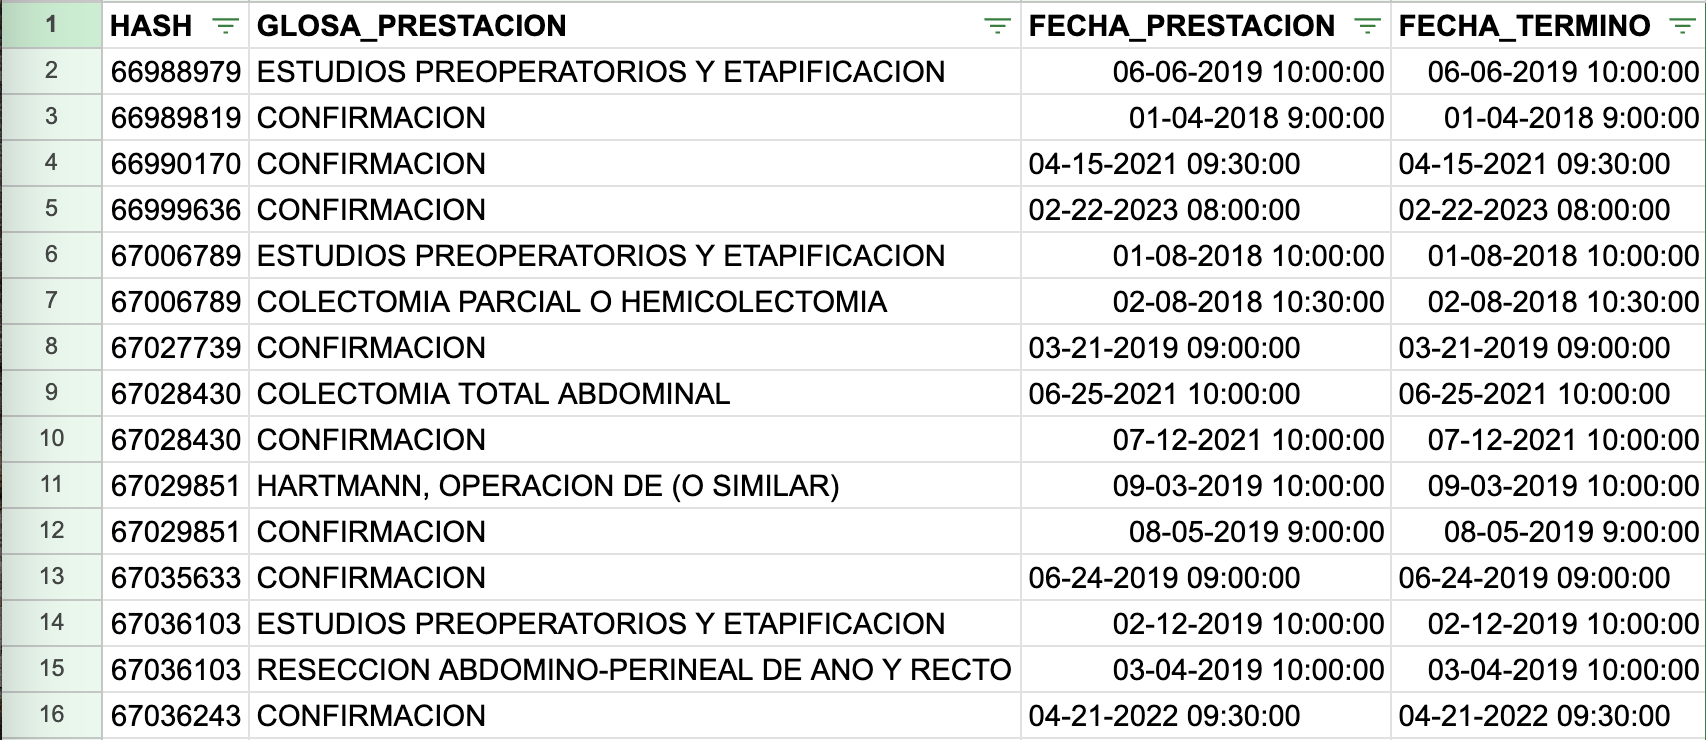
\includegraphics[width=1\textwidth]{images/3.methodology/benefits_dataset.png}
    \caption{Benefits Dataset}
    \label{fig:benefits_dataset}
\end{figure}

As depicted in Figure \ref{fig:benefits_dataset}, the first dataset meticulously outlines the specific benefits of the GES program accessed by each patient in the district over a five-year period, offering a detailed view of each patient's journey with the disease. However, a limitation of this dataset lies in its provision of only the initiation date for each benefit.

\begin{figure}[H]
    \centering
    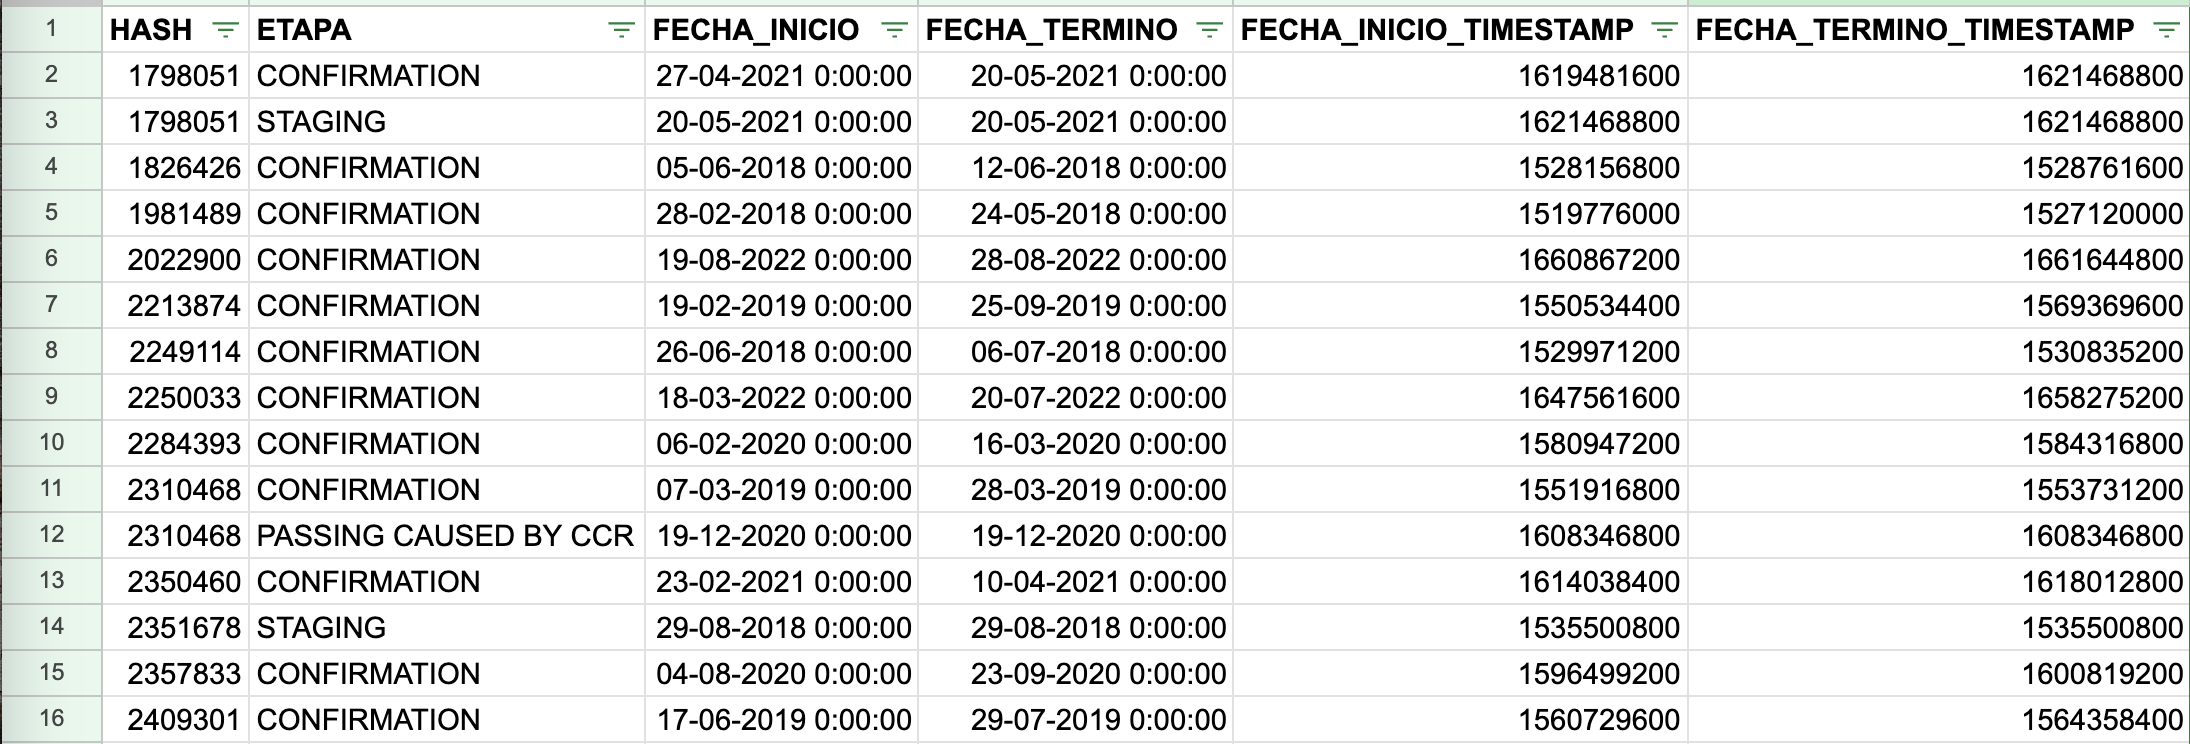
\includegraphics[width=1\textwidth]{images/3.methodology/stages_dataset.png}
    \caption{Stages Dataset}
    \label{fig:stages_dataset}
\end{figure}

In contrast, as seen in Figure \ref{fig:stages_dataset}, the second dataset focuses specifically on the stages undergone by patients during their diagnosis and treatment of CRC in a six-year period, covering confirmation, staging, and treatment phases. This dataset provides both the start and end dates for each stage, enabling the calculation of the duration of each phase.


\begin{table}[H]
\caption{Original Database Overview}
\centering
\begin{tabular}{|c|c|c|c|c|}
\hline
DB & Patients & Source & Initial Data & Final Date\\ \hline
GES Benefits & 3648 & SIGGES & 12/03/2013 & 19/05/2023\\ \hline
GES Stages & 2989 & SIGGES & 4/10/2017  & 23/09/2023\\ \hline
\end{tabular}
\label{table:original_database_overview}
\end{table}


As indicated in Table \ref{table:original_database_overview}, each dataset contains a sufficient number of patients to perform a successful PM analysis. This suggests that the SIGGES database can easily support a two-level abstraction approach for studying each disease using PM.

The second dataset included information regarding the deaths of individuals, with distinctions made between those associated with CRC and those resulting from other causes. This additional information, vital for a comprehensive understanding, was extracted from the cause of death records within the government's databases, ensuring the inclusion of patient mortality data in our analysis.

\label{sec:data_preprocessing}
\subsection*{Data Preprocessing}

The first step of the process was case and activity filtering based on the rules described in the MEDCP methodology \cite{vathy-fogarassy_multi-level_2022}. 

\begin{itemize}

    \item {Standardized date formats.}

    \item {Separated activities with the same timestamp by a small margin according to their logical order.}

    \item {Stacked activities in the Benefits dataset that were performed in a sequence without interrumption.}

    \item {Removed all activities not related to the diagnosis or treatment of the disease.}

    \item {Deleted events outside of the analysis period.}

    \item {Removed uncommon patient sequences.}

    \item {Removed unimportant treatment and diagnosis events.}
\end{itemize}
 

For the Benefits database, only cases that started before 2023 and had a stage sequence repeated more than 10 times were considered. Additionally, benefits that were delivered more than 40 times and provided since 2018 were included.

For the Stages database, only cases that started before 2023, had a stage sequence repeated more than 10 times, and had their treatment started before 2019 were considered.

The results of this process are shown in Table \ref{table:preprocessed_database_overview}.

\begin{table}[H]
\caption{Preprocessed Database Overview}
\centering
\begin{tabular}{|c|c|c|c|c|}
\hline
DB & Patients & Source & Initial Data & Final Date\\ \hline
GES Benefits & 2048 & SIGGES & 01/01/2018 & 22/09/2023\\ \hline
GES Stages & 2524 & SIGGES & 15/11/2017  & 23/09/2023\\ \hline
\end{tabular}
\label{table:preprocessed_database_overview}
\end{table}

\subsection*{Process Mining Results}

Our initial investigation aims to examine the different stages of the process to identify common pathways and quantify the number of individuals entering and exiting each stage. Figure \ref{fig:stages_in_disco} depicts the process map, encompassing 100\% of the activities and paths.

\begin{figure}[H]
    \centering
    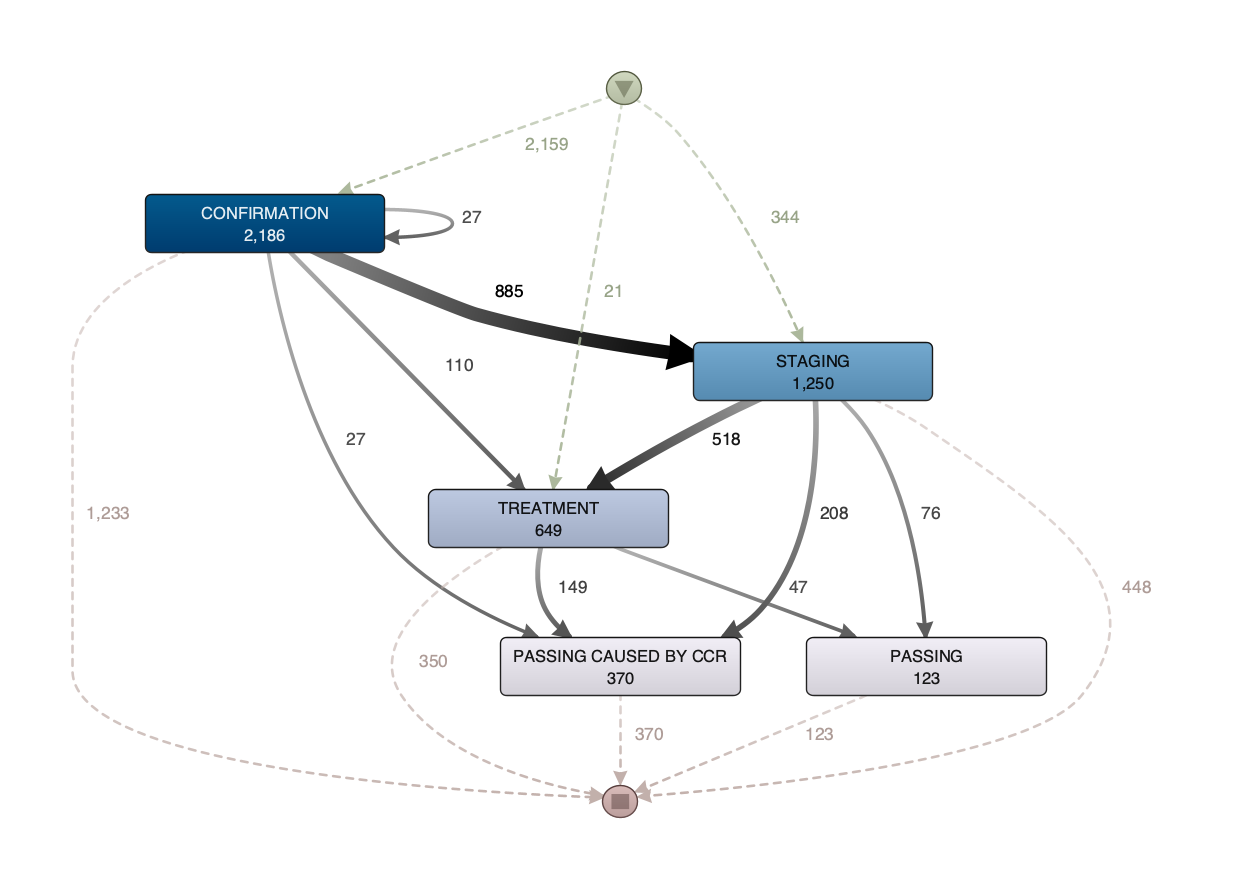
\includegraphics[width=1\textwidth]{images/3.methodology/stagesCRC.png}
    \caption{Stages of CRC in Disco}
    \label{fig:stages_in_disco}
\end{figure}


The process map in Figure \ref{fig:stages_in_disco} provides a compelling visual representation of the patient journey through various stages of care. The majority of patients progress solely to the Confirmation stage, signalling most of them were not confirmed with the disease, as evidenced by the relatively low number of CRC-related passings. Notably, nearly half of these individuals proceed to the Staging stage, indicating a substantial subset of patients being confirmed with CRC. From there, 518 patients advance to the Treatment stage, showing a notable proportion opting for treatment within the public healthcare system. However, it's noteworthy that a portion of patients might opt for alternative avenues, such as seeking care in the private sector or choosing not to undergo treatment at all.

Next, we are going to look into the specific benefits that were given to the patients. Figure \ref{fig:benefits_in_disco} illustrates the process map, encapsulating 100\% of the activities and 20\% of the paths.

\begin{figure}[H]
    \centering
    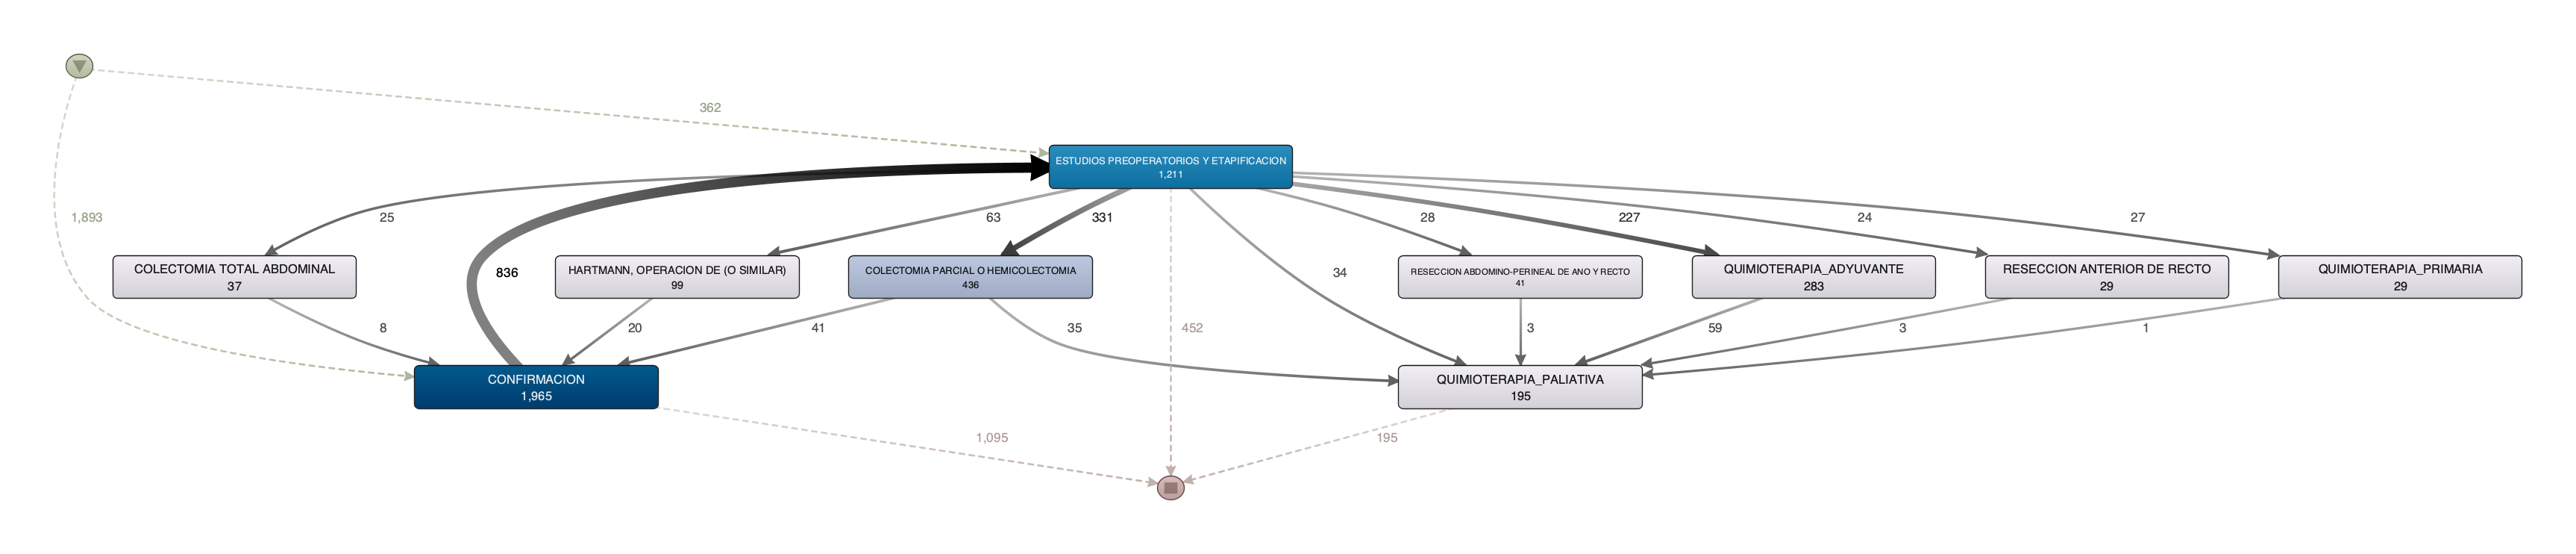
\includegraphics[width=1\textwidth]{images/3.methodology/benefits100_20.png}
    \caption{Benefits delivered to CRC Patients in Disco}
    \label{fig:benefits_in_disco}
\end{figure}

As this visual representation is difficult to analyze, the activities were reduced to 60\% and the paths were kept at 20\%.

\begin{figure}[H]
    \centering
    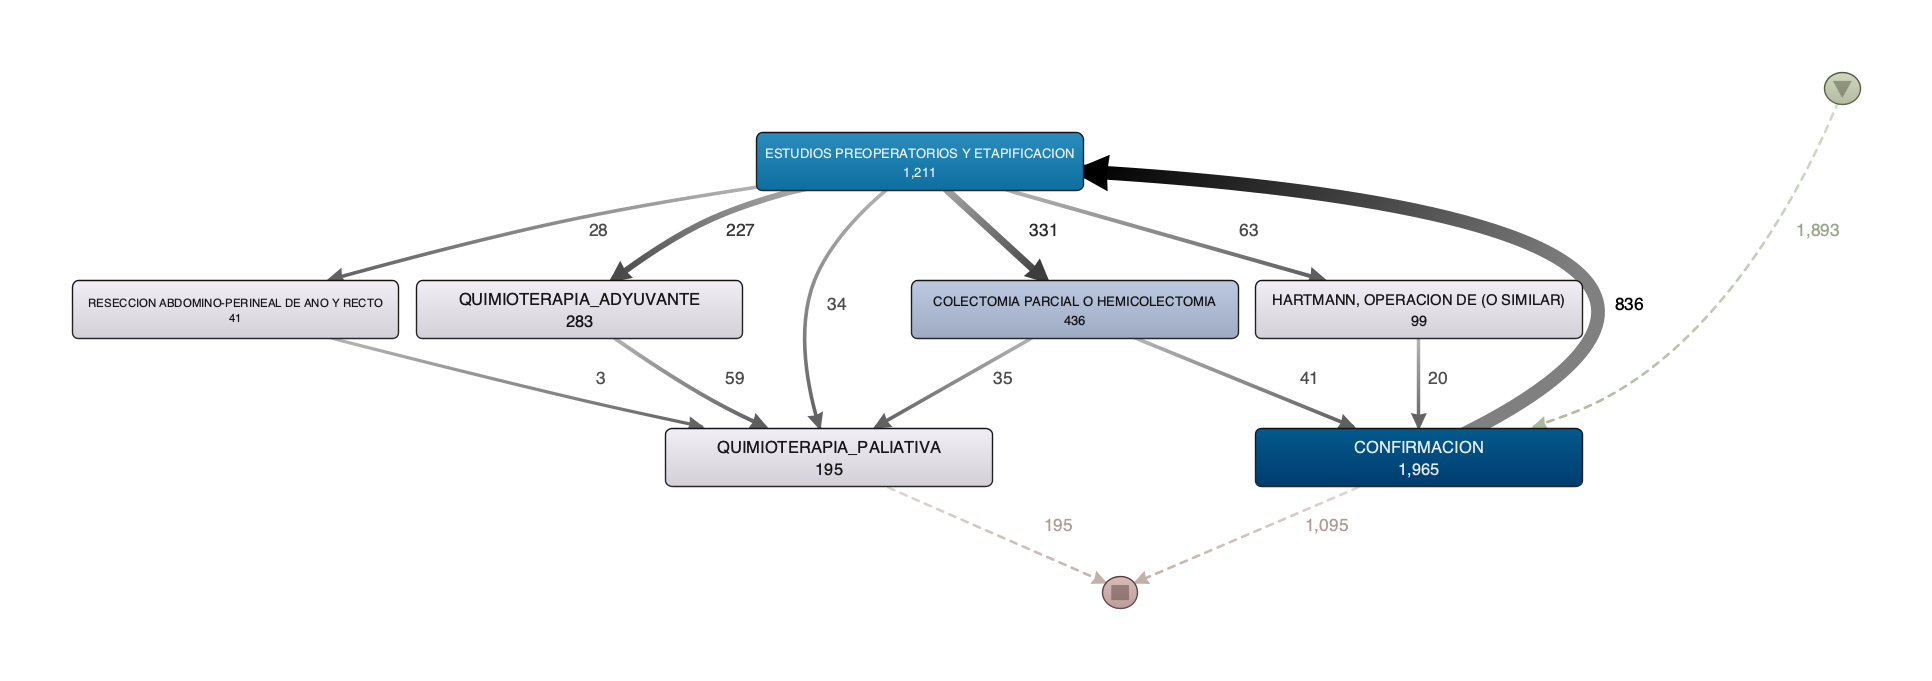
\includegraphics[width=1\textwidth]{images/3.methodology/benefits60_20.png}
    \caption{Benefits of CRC in Disco Activities at 60\% and Paths at 20\%}
    \label{fig:benefits_60_in_disco}
\end{figure}

As depicted in Figure \ref{fig:benefits_60_in_disco}, the generated process map illustrates the typical benefits received by patients undergoing CRC care. Initially, they go through the Confirmation and Staging stages, followed by receiving treatment. This treatment typically encompasses surgical interventions such as colectomy, Hartmann procedure, or abdominoperineal resection, along with adjunctive or palliative chemotherapy.

\subsection*{Insights from the MND Team}

Examining both process maps offers a glance into the prevalent pathways in CRC care. However, relying only on them offers a nearsighted picture of the current state of CRC treatment within the SMPHS. To widen our perspective into the intricacies of diagnostic and treatment processes for CRC, the insights provided by the MND team are indispensable.

The following Figure \ref{fig:process_overview} presents the diagnostic and treatment process for CRC, as viewed through the lens of the MND team:

\begin{figure}[H]
    \centering
    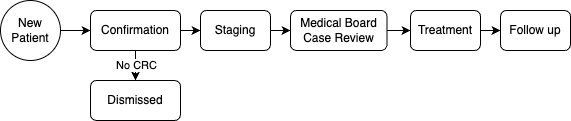
\includegraphics[width=1\textwidth]{images/3.methodology/ProcessOverview1.drawio.png}
    \caption{Process Overview according to the MND team}
    \label{fig:process_overview}
\end{figure}

Following are detailed descriptions of each process based on insights gathered from interviews with the MND team:

\begin{description}
   \item[Suspicion] A patient arrives at a public healthcare facility exhibiting symptoms suggestive of CRC, such as rectal bleeding, diarrhea, constipation, abdominal pain, weight loss, or anemia. While these symptoms may indicate other conditions, practitioners suspect CRC and refer patients to Barros Luco Hospital, the only facility equipped for colonoscopies within the Service.
   
   \item[Confirmation] Upon suspicion of CRC, patients undergo colonoscopy, with scheduling prioritized based on urgency. Some patients receive immediate scheduling, while others are placed on a waiting list. Barros Luco Hospital is the sole facility within the SMPHS equipped to perform colonoscopies, with a specialized team dedicated to this purpose.
   
   \item[Staging] Following CRC confirmation, patients undergo additional exams, including blood and imaging tests. Blood exams provide crucial insights into the patient's condition, guiding surgical decisions, while imaging tests help determine the required procedure.
   
   \item[Medical Board Review] This stage is not directly captured in the Benefits or Stages dataset. However, it plays a critical role in the treatment process. The case is presented to a Medical Board responsible for determining the most suitable treatment plan. It's important to note that not all treatments aim for a cure; some are palliative, especially for patients with advanced cancer stages. This stage begins when the results of the Staging exams are available and concludes when the board reaches a resolution.
   
   \item[Treatment] The Treatment phase begins when the Medical Board concludes its review and ends when the first treatment procedure is initiated. The treatment typically involves chemotherapy/radiotherapy and/or surgical procedures.
   
   \item[Follow-up] Following the completion of treatment, patients participate in yearly follow-up meetings for at least the next five years, or longer based on their individual circumstances.
\end{description}

This comprehensive analysis, informed by insights from the MND team, provides a detailed perspective on the CRC care process within the Service. Remarkably, certain stages are absent from the process maps. The suspicion stage is not represented due to the GES system's initiation upon suspicion, making this phase irrelevant to GES guarantees. However, the absence of metrics for the Medical Board Review stage raises concerns regarding its influence on overall process performance. Furthermore, the Follow-up stage was deliberately omitted from the data analysis due to a lack of sufficient cases, as discussed in the \hyperref[sec:data_preprocessing]{Data Preprocessing} subsection.

\subsection*{Performance Metrics}

The government has instituted specific timelines for the completion of each stage within the CRC care process by law, as outlined in Figure \ref{fig:government_kpis}. The decision to investigate this particular disease was influenced by the MND team's observation that the compliance percentage with these designated time frames consistently lagged behind for CRC. This emphasis on time frames underscores the significance of addressing potential delays in the diagnostic and treatment phases to improve overall healthcare efficiency.

\begin{figure}[H]
    \centering
    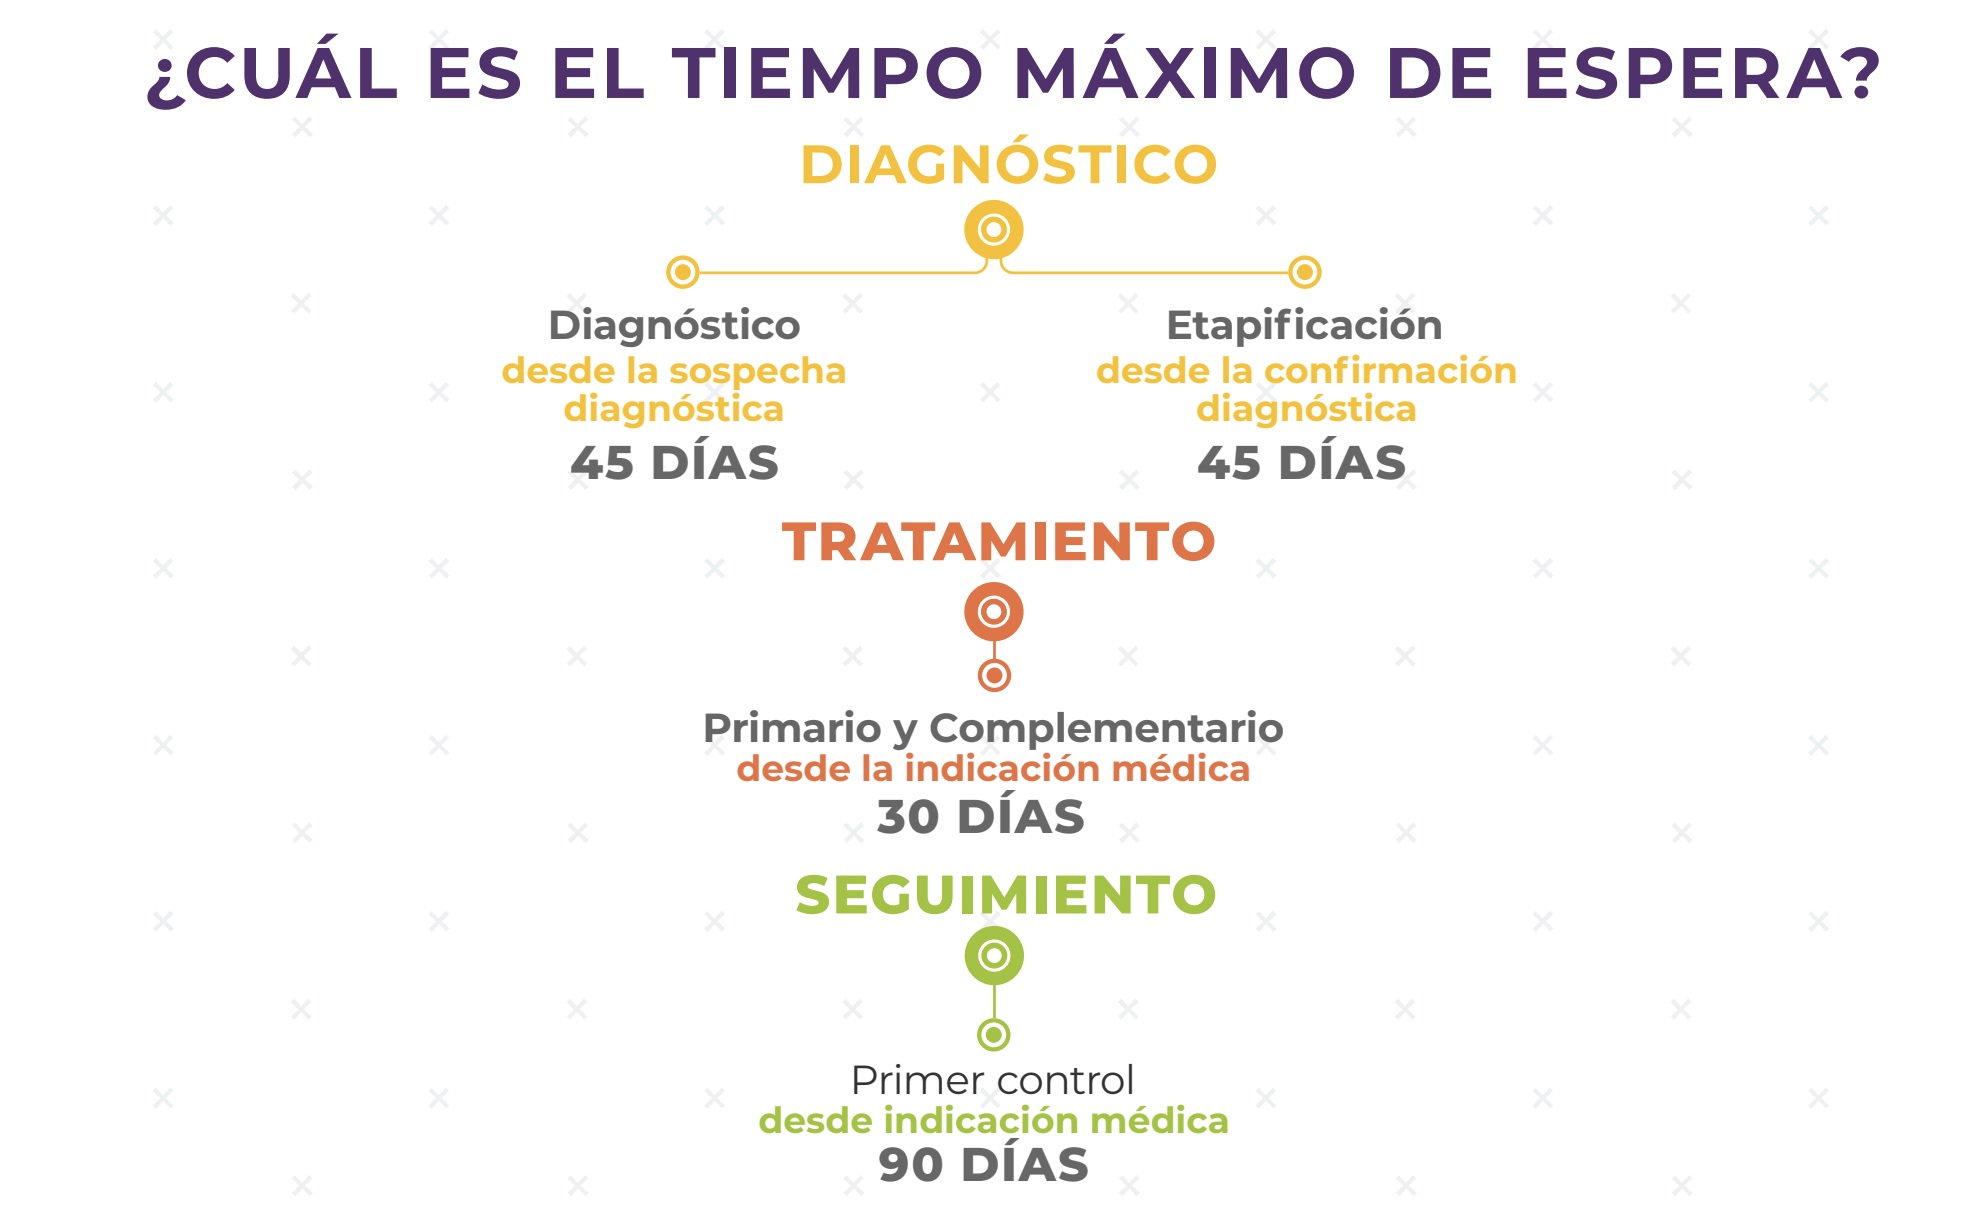
\includegraphics[width=1\textwidth]{images/3.methodology/KPIGobierno.png}
    \caption{Government-mandated stage Time Frame for CRC Diagnosis and Treatment\textsuperscript{1}}
    \label{fig:government_kpis}
\end{figure}

\footnotetext[\value{footnote}]{From \textit{Cáncer Colorectal en
Personas de 15 años y más}. Superintendencia de Salud, 2023. \url{https://www.superdesalud.gob.cl/difusion/665/articles-18886_archivo_fuente.pdf}}

Figure \ref{fig:government_kpis} illustrates the time frame requirements mandated by the government for the diagnostic phase of colorectal cancer care. Both the Confirmation and Staging stages must be completed within 45 days of the initial suspicion and diagnostic confirmation. Subsequently, treatment initiation is mandated to commence within 30 days of the medical order. Following treatment completion, the first follow-up meeting should be scheduled within 90 days.

\begin{table}[H]
\caption{Government-mandated Time Frame compliance}
\centering
\begin{tabular}{|c|c|c|}
\hline
 & N & On-time(\%)\\ \hline
Confirmation & 2552 & 1462 (57.28\%)\\ \hline
Staging &      1435 & 1204 (83.9\%)\\ \hline
Treatment &    933  & 519 (55.62\%)\\ \hline
Follow-up &    168  & 108 (64.28\%)\\ \hline
\end{tabular}
\label{table:government_kpis_compliance}
\end{table}

Table \ref{table:government_kpis_compliance} provides insights into the timeliness of CRC care stages. Notably, the Confirmation and Treatment stages consistently lag behind the designated time frames. In contrast, the Staging process generally meets the expected timelines. This highlights the need for focused efforts to improve efficiency in the Confirmation and Treatment stages, ultimately enhancing adherence to prescribed timelines and improving care for CRC patients.

\section{Process Analysis}

The process analysis builds upon the information presented in the previous section, with a distinct emphasis on the invaluable contribution of the MND team. Combining the information gathered from the understanding of the CRC care process, performance metrics, scientific research and medical advice provided enough evidence to suggest issues and a potential improvement strategy for the SMPHS.

Furthermore, the collaborative approach aims to guarantee that the proposed improvements are not only identified accurately but are also pragmatic in terms of implementation difficulty and the available resources. This collaborative perspective enriches the process analysis, aligning it with the identified challenges and offering feasible solutions within the context of the Southern Metropolitan district's healthcare system.

\subsection*{Current Issues}

This research stage was approached with care due to the little experience the investigator had in the medical and operational field. Every idea that came up was discussed with the MND team to validate if it was indeed an issue for the SMPHS.

\subsubsection*{Poor Performance in the Confirmation Stage}

Figure \ref{fig:confirmation_stage} displays the Stages process map, isolating the cases where the Confirmation activity is involved. One notaworthy observation from this analysis is the significant proportion of patients progressing only through the Confirmation stage. As depicted in the "CONFIRMATION" activity in Figure \ref{fig:confirmation_stage}, approximately 56.4\% of patients exit the CRC care process after Confirmation. This departure should mostly be attributed to negative colonoscopy results. However, this trend may indicate data incompleteness, particularly in the cases where patients transition from the "CONFIRMATION" activity to "PASSING CAUSED BY CRC", creating uncertainty about their treatment status. These patients likely received a positive CRC result but may have opted for treatment in the private sector or no treatment at all.

\begin{figure}[H]
    \centering
    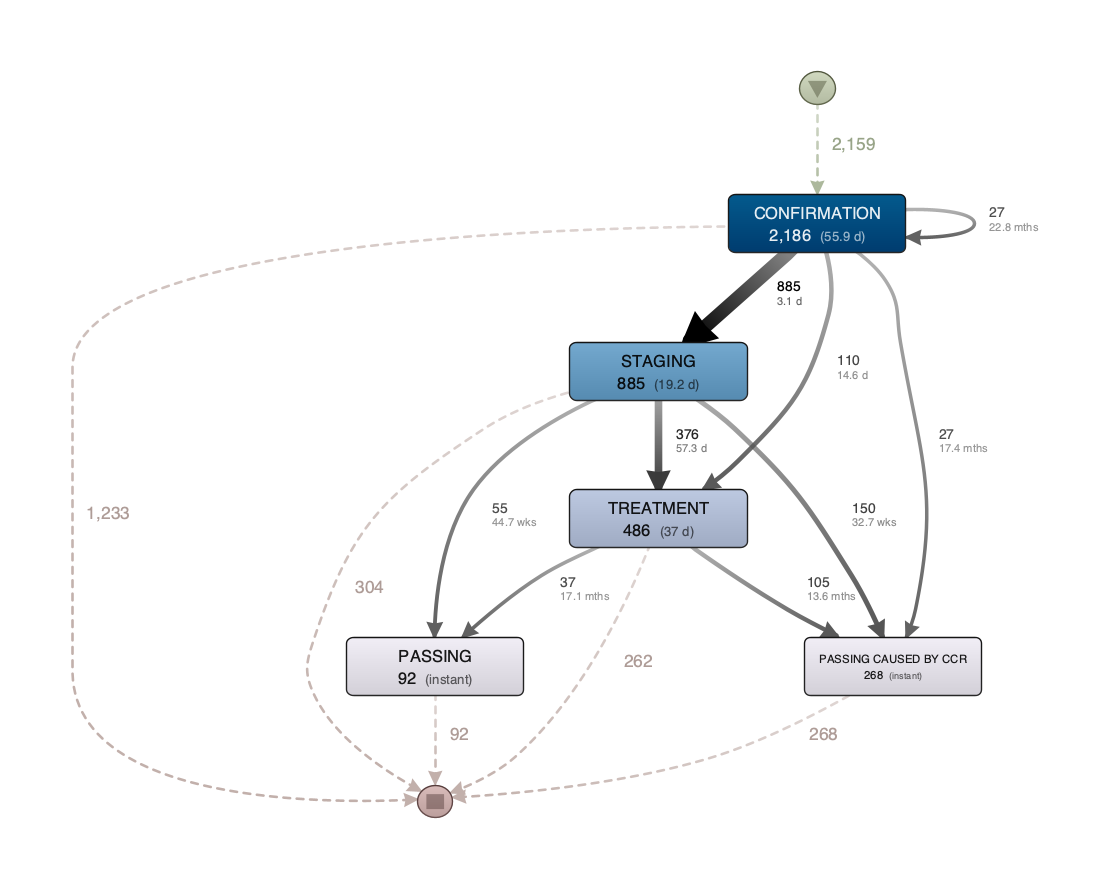
\includegraphics[width=1\textwidth]{images/3.methodology/confirmation_stage.png}
    \caption{Confirmation Stage in Disco}
    \label{fig:confirmation_stage}
\end{figure}

As shown in Table \ref{table:government_kpis_compliance}, a notable concern regarding the Confirmation stage is that only 57.28\% of confirmations occur within the prescribed time frame. Furthermore, as illustrated in the "CONFIRMATION" activity on Figure \ref{fig:confirmation_stage}, the average waiting time for CRC diagnosis confirmation extends to 55.9 days. 

\begin{figure}[H]
    \centering
    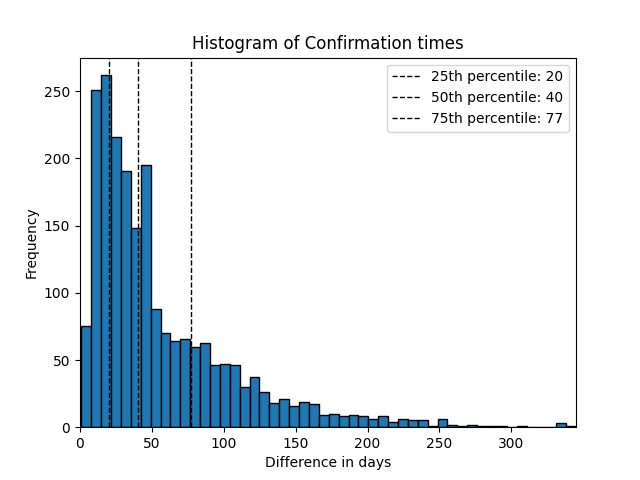
\includegraphics[width=1\textwidth]{images/3.methodology/confirmation_histogram.png}
    \caption{Confirmation Histogram}
    \label{fig:confirmation_histogram}
\end{figure}

In Figure \ref{fig:confirmation_histogram}, we observe that a quarter of patients receive their confirmation results in 20 days or less, while another quarter wait for more than 77 days. While this duration may not significantly affect disease progression given CRC's long sojourn time, it undoubtedly causes discomfort for patients and their families.

Given this performance, one has to consider the colonoscopy capacity of the SMPHS. In 2020, the population of the Netherlands was approximately 17.4 million people, and the number of colonoscopies performed was 44,036 \cite{noauthor_national_nodate}. This translates to 0.0025 colonoscopies per person. Considering that the Netherlands has one of the best healthcare systems for CRC prevention \cite{navarro_colorectal_2017}, the SMPHS, with a population of approximately 1.1 million, should be performing 2,750 colonoscopies every year. However, based on the Stages dataset covering about 4.85 years, the SMPHS is currently performing approximately 526 colonoscopies annually.

Beyond its potential impact on disease management, this observed pattern is indicative of the current confirmation stage performance. Most patients receive confirmation results after a prolonged period following CRC suspicion, likely due to limited resources for coloscopy procedures. This prolonged waiting period affects patient morale and their readiness to undergo future diagnostic and treatment procedures critical to their overall well-being.

\subsubsection*{Missing treatments}

Figure \ref{fig:staging_stage} displays the Stages process map, isolating the cases where the Staging activity is involved. A notable trend from previous chapters is the significant number of patients who discontinue their progression through the CRC care process, particularly after the Confirmation and Staging activities. As depicted in the "STAGING" activity of Figure \ref{fig:confirmation_stage}, only 376 out of 885 individuals (42.49\%) who completed both activities received treatment in the public sector. Similarly, in Figure \ref{fig:staging_stage}, only 511 out of 1250 individuals (40.88\%) who went through the "STAGING" activity continued with the "TREATMENT" activity.

\begin{figure}[H]
    \centering
    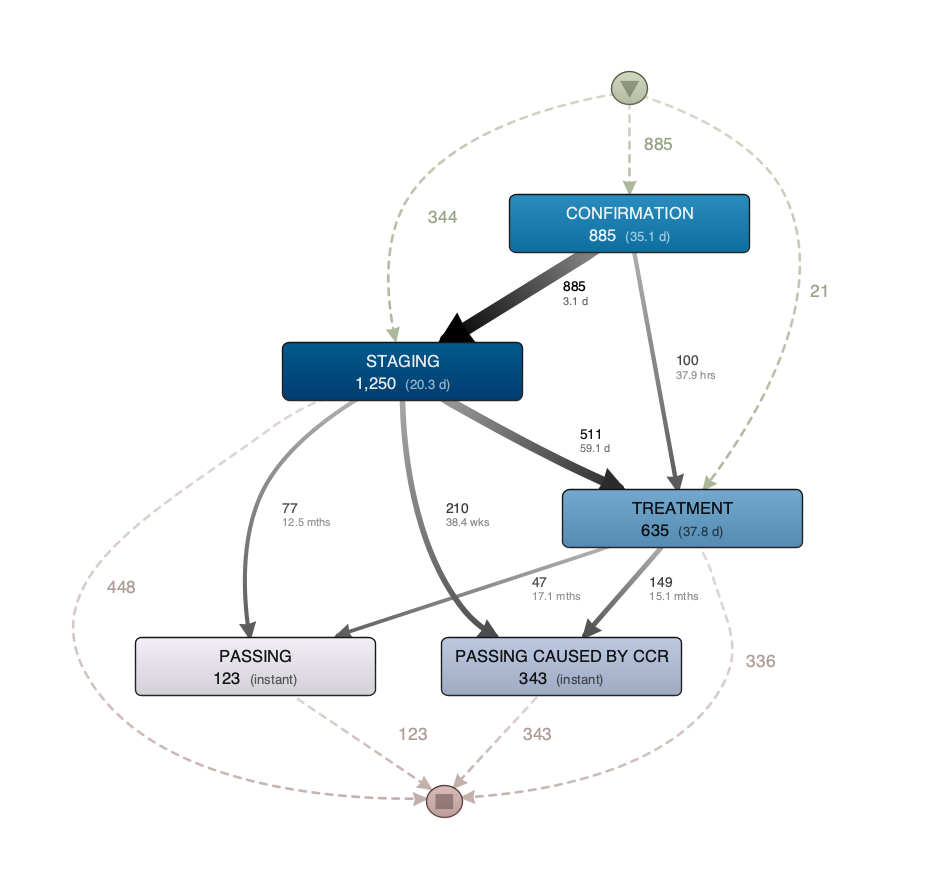
\includegraphics[width=1\textwidth]{images/3.methodology/staging_stage.png}
    \caption{Staging Stage in Disco}
    \label{fig:staging_stage}
\end{figure}

This concerning trend highlights the public sector's struggle to deliver timely and efficient treatment, emphasizing the pressing need to improve the healthcare system's responsiveness. The harsh reality is that a considerable number of patients are opting to halt their treatment for reasons yet to be determined.

Figure \ref{fig:complete cases} shows a process map where the only cases that were kept where those were the starting activity was "CONFIRMATION" and their end activity was either "TREATMENT", "PASSING" or "PASSING CAUSED BY CRC".

\begin{figure}[H]
    \centering
    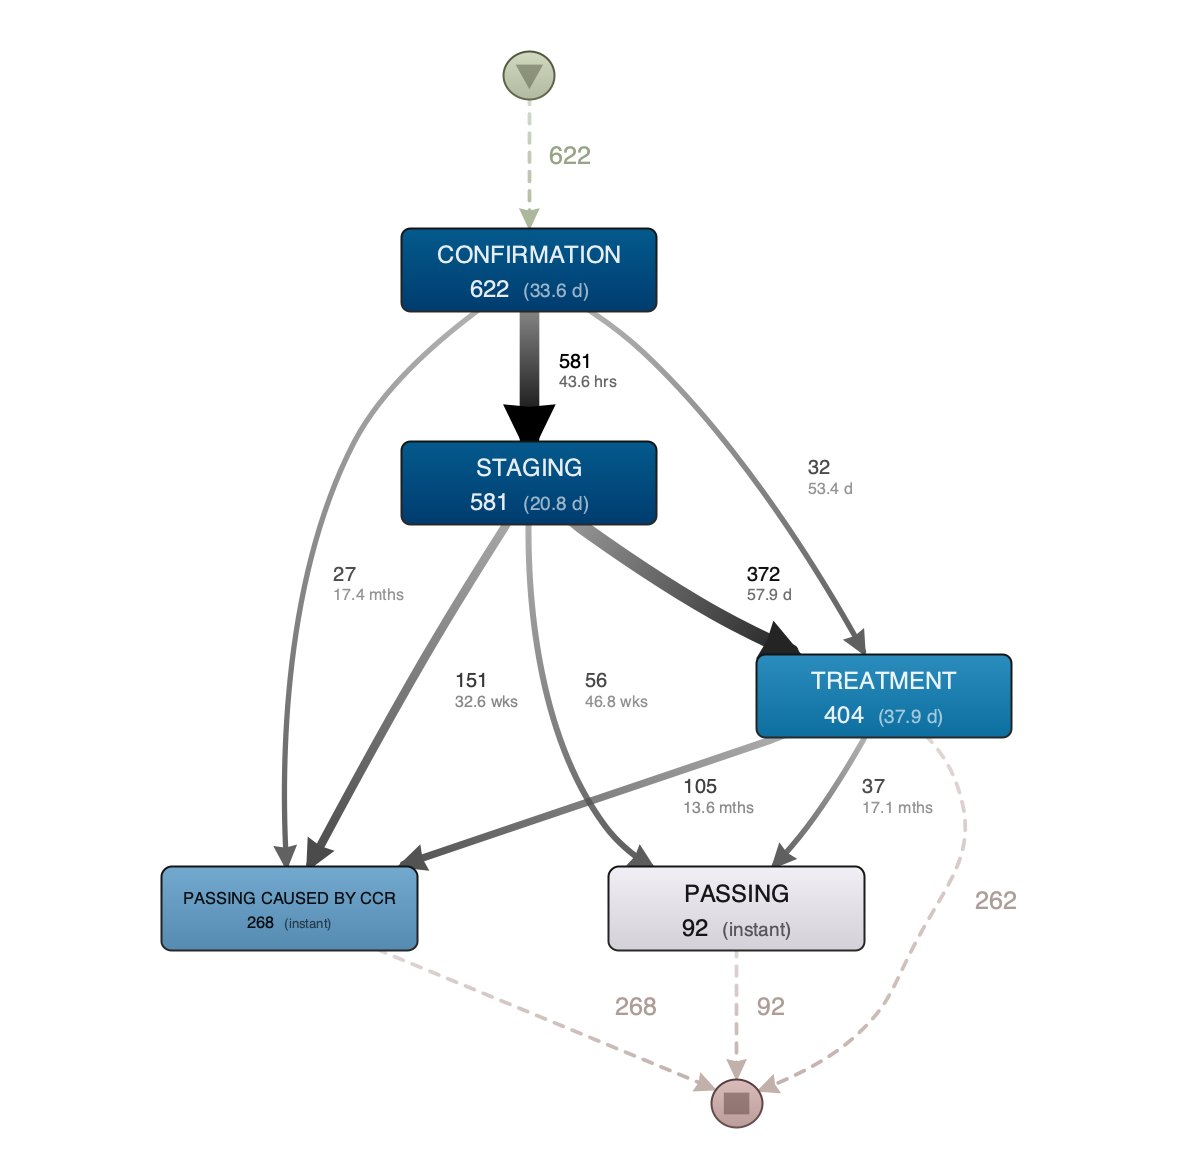
\includegraphics[width=1\textwidth]{images/3.methodology/complete_cases.png}
    \caption{Complete Cases in Disco}
    \label{fig:complete cases}
\end{figure}

It's worth noting that, on average, the sum of waiting times across all activities preceding the start of treatment ("CONFIRMATION", "STAGING" and "TREATMENT" amounts to 152 days (33.6+1.8+20.8+57.9+37.9), roughly equivalent to 5 months from the initial suspicion to treatment commencement. This prolonged timeline highlights the urgent need for expedite access to treatment within the public sector to improve outcomes and reduce the risks associated with delayed intervention.

\subsubsection*{Lack of preventive medicine}

A key insight, emphasized by both the MND team and supported by the literature review, is the importance of preventive medicine in the Chilean public healthcare system. According to a survey conducted in Chile with 1893 respondents, as reported by \citeA{alfaro_barriers_2024}, 79.6\% of the respondents stated they had never undergone any form of CRC screening, and 90.4\% had not been screened for CRC in the last three years.  Interestingly, among respondents with private insurance (26.8\% of the total), screening rates were better, indicating a potentially even worse situation within the SMPHS.

This data implies that nearly all patients seeking care within the public sector are diagnosed as symptomatic patients, meaning their diagnosis occurred after they had already exhibited signs of the suspected disease. It is widely agreed among researchers that implementing screening methods is a critical step toward improving the prognosis for CRC patients \cite{van_rossum_earlier_2009, soerjomataram_most_2012}.

\begin{figure}[H]
    \centering
    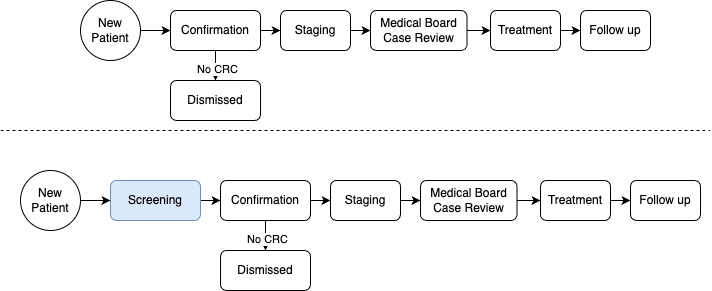
\includegraphics[width=1\textwidth]{images/3.methodology/ProcessOverview2.drawio.png}
    \caption{Diagnosing and treating patients with Screening Stage}
    \label{fig:process_overview_2}
\end{figure}

Figure \ref{fig:process_overview_2} depicts the Process Overview with an additional Screening activity. Currently, the most effective screening methods involve detecting blood in fecal matter, with widely used tests like the fecal occult blood test (FOBT) and the fecal immunochemical test (FIT) showing consistent improvement over the years. These tests have been successfully integrated into numerous public healthcare systems, most of them from Europe \cite{navarro_colorectal_2017}. 

Most preventive strategies revolve around using these exams to determine eligibility for periodic preventive colonoscopies, offering the tests annually. Some strategies also consider providing preventive colonoscopies every five or ten years, but this approach is often considered expensive due to the increased number of required colonoscopies resulting from false positives. The majority of researched strategies recommend initiating these screenings at age 50.

Compelling evidence suggests that implementing these preventive strategies can lead to cost savings in certain scenarios \cite{lansdorp-vogelaar_effect_2009}. This cost-saving effect is primarily attributed to the early detection of cancerous tumors at an asymptomatic stage, which results in less advanced disease and subsequently reduces the costs associated with treatment. Nonetheless, a major challenge remains in persuading the population to undergo regular preventive screenings, thereby promoting early detection and intervention.

\subsection*{Potential Improvement Strategy}

Crafting an effective improvement strategy poses a formidable challenge, particularly given that the main issues can be summarized as a process with poor time delivery performance. This means that there is not a clear path for improvement but the objective is to streamline the delivery of diagnosis results and treatments. The complexity intensifies as the resources for the SMPHS are limited, therefore any increase in the CRC care budget has to be properly justified. 

The delayed Confirmation and Treatment stages reveal the overburden of the SMPHS in the CRC care process. It is unclear whether the care units involved need more resources or if the optimization of existing resources is required. However, it is evident that both are failing to meet their objectives on time.

Addressing the issue of missing treatments is crucial for the improvement strategy, as it strongly suggests dissatisfaction with the public healthcare system's performance. To rectify this, one of the strategy's most important objectives must be to enhance the overall performance of the diagnostic and treatment process, instilling confidence in patients to continue treatment within the public healthcare system.

Considering the lack of preventive medicine, the poor performance of the CRC care process and the advice of the MND team, the implementation of a Screening stage emerges as a valid proposal for an improvement strategy. This reallocation of resources from treatments to diagnosis can improve CRC prognosis and potentially result in cost savings. However, it's important to note that this strategy does not directly address the main issues currently affecting the SMPHS's CRC care process, which are primarily related to a lack of resources and/or inefficient use of them.

The subsequent chapters will simulate and calculate the potential costs and benefits associated with implementing a Screening stage in the current CRC care process of the SMPHS.



\chapter[Simulation]{Simulation}
\label{chapter:simulation}
In this chapter, we explore the construction and implementation of a simulation designed to evaluate the proposed improvement strategy for the CRC care pathway within the Southern Metropolitan Public Healthcare System. This simulation serves as a crucial tool in assessing the feasibility, costs, and potential outcomes of the proposed enhancements outlined in the preceding chapters.

The simulation model was written entirely on Python. All of its code is available on this public github repository.

\url{https://github.com/Tomasalvarez15/crc_screening_simulator}

\section{Simulation Framework Selection}

The selection of framework for the simulation model started with a revision of the available type of models for this kind of simulation. A recent study found 43 other studies which used a simulation model to validate a screening strategy for CRC \cite{smith_simulation_2020}. Of them the most used kind of model was Markov modeling (72\%), Monte Carlo modeling (16\%) and microsimulation (14\%). It is important to note that some studies used more than one kind of model. 33\% of the studies cited the MISCAN-Colon model \cite{loeve_miscan-colon_1999} as their base model.

The other simulation models considered did not align with the specific requirements of this study. The Markov model, for instance, lacks the capability to incorporate dynamic disease progression and is not easily scalable over the long term. Given the objective of accurately representing the natural history of colorectal cancer, this model was deemed unsuitable. Similarly, Monte Carlo simulations sequentially run each individual's life, making them less conducive to simulating all individuals simultaneously, as desired for this investigation. While Discrete Event Simulation (DES) was a viable option, its focus on how individual actions impact the system differs from the individual-centric approach of microsimulation. Consequently, microsimulation emerged as the preferred simulation type for this study due to its emphasis on capturing the nuanced dynamics of individual experiences within the broader healthcare system.

\section{Microsimulation Model Operational Explanation}

The microsimulation model functions as a virtual population filled with individuals. It begins at a specified starting year and progresses until a set number of years have elapsed, collecting statistics for later analysis. The simulation depicts the lives of individuals in the population, modeling the screening process for those who undergo it and simulating the natural history of CRC for those who develop the disease. Individuals who do not fall into these categories remain in the simulation without active interaction until their simulated death.

Next, each component of the simulation's structure and processes will be explained in detail.

\subsection*{Structure of the Simulation Objects}

The microsimulation has two main structures. The population and the individuals. Each of them have specific properties and functions that allow the simulation to represent the behaviour of CRC care.

\begin{figure}[H]
    \centering
    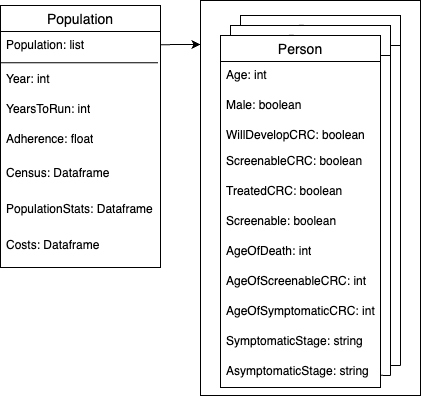
\includegraphics[scale=0.6]{images/4.simulation/ClassDiagram.png}
    \caption{Structure of the Simulation Objects and their Attributes with Types}
    \label{fig:structure_of_the_simulation_objects}
\end{figure}

The diagram in Figure \ref{fig:structure_of_the_simulation_objects} shows the essential data retained by the Population object. Firstly, it includes a list of all individuals. Secondly, it contains the current year and adherence percentage for generating new individuals. Thirdly, it tracks the remaining years to determine the simulation's end. Fourthly, it maintains the Census, PopulationStats, and Costs DataFrames for recording yearly statistics like age distributions, activity records, and operational costs.

Each Person object encapsulates all required information to depict an individual's current state, encompassing factors such as age, sex, anticipated age of death, and pertinent variables concerning CRC diagnosis and progression.

\subsection*{Instantiating a Person Object}
 

When creating a Person object, certain attributes are pre-set, while others are determined by random uniform distributions. If these attributes fall below specific parameters, they are assigned one value; otherwise, they are assigned another.

\begin{figure}[H]
    \centering
    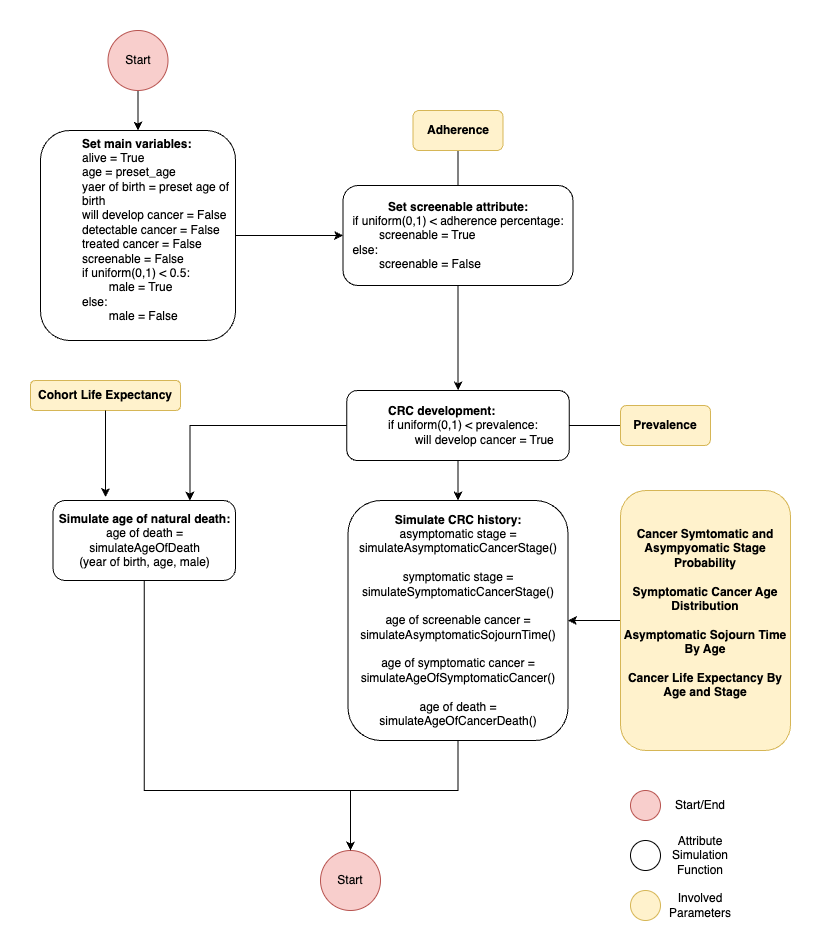
\includegraphics[scale=0.4]{images/4.simulation/InstantiatingAPerson.png}
    \caption{Instantiating a Person Object Process}
    \label{fig:instantiating_a_person}
\end{figure}

As shown in Figure \ref{fig:instantiating_a_person}, several parameters are considered when simulating each individual's life. Once created, their attributes are set, including the ages at which they will experience changes in status.

\begin{figure}[H]
    \centering
    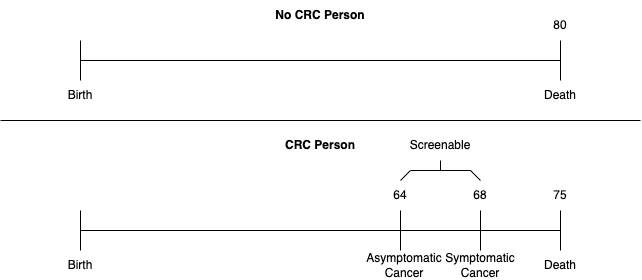
\includegraphics[width=1\textwidth]{images/4.simulation/NaturalHistoryDiagram.png}
    \caption{Person Life History from the Simulation}
    \label{fig:natural_history}
\end{figure}

In Figure \ref{fig:natural_history}, individuals without CRC experience no status changes except for their eventual death at a specified age. However, for those with CRC, a positive screening result within the screenable interval recalculates their life expectancy. Detecting CRC earlier extends their life, recorded as years gained from screening. If their life expectancy decreases due to a later asymptomatic stage, the years are subtracted from the total.

\subsection*{Yearly Progression Overview}
The program progresses through each year (iteration), checking and updating the health status of each person in the population. This process repeats for each simulated year, allowing researchers to observe how different screening strategies impact the overall CRC outcomes in the population over time.

The decision to run the microsimulation in one-year intervals balances capturing meaningful changes in CRC progression with maintaining computational efficiency. While shorter intervals would increase complexity and computational load, this enhancement could be added to the simulation model in the future.

\begin{figure}[H]
    \centering
    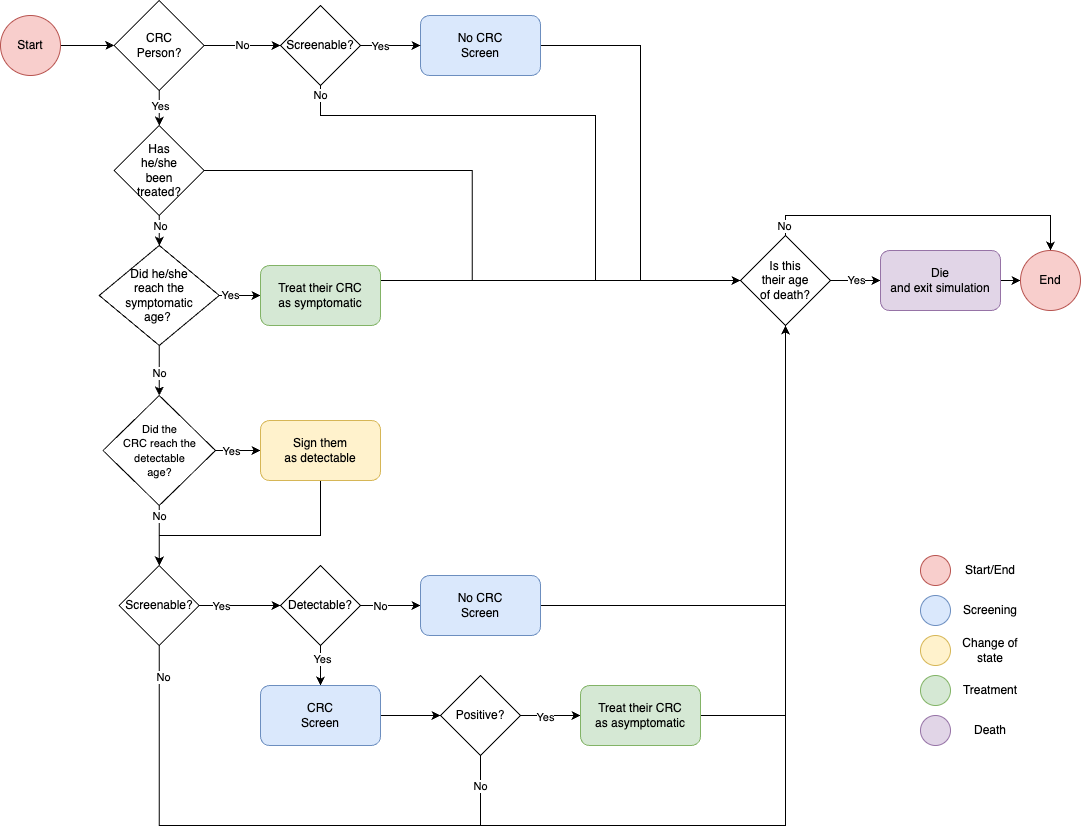
\includegraphics[width=1\textwidth]{images/4.simulation/simulation_person_process.png}
    \caption{Person Processing Flowchart}
    \label{fig:simulation_person_processing}
\end{figure}

Each year, every individual undergoes the process depicted in Figure \ref{fig:simulation_person_processing}. In the first step, this pathway segregates those with CRC in their natural history.

For individuals without CRC, their significance lies primarily in the statistics of screening strategies, as the majority of screenings are conducted on individuals who will never develop CRC.

For those with CRC in their natural history, their course of action depends on the stage of their disease and whether they are screenable. They may undergo screening and/or treatment either symptomatically, when the disease manifests symptoms, or asymptomatically, when CRC is detected through the screening process. If this happens, their age of death will be updated according to their asymptomatic stage.

\section{Simulation Parameters}
\label{section:simulation_parameters}

For the simulation to be accurate, multiple data is needed in various aspects. Initially, we will examine demographic data, followed by data related to the CRC disease, and finally, the costs of procedures for the economic analysis.

\subsection{Demographic Data}

For demographic data, the initial population was obtained from the studied region, and the population projection from Chile was available. However, the best publicly available information for cohort life expectancy came from the US. Replacing this data with sources from Chile, ideally from the studied region, is an important endeavor for improving the accuracy of the simulation.


\subsubsection*{Initial Population}

To simulate the current population the MND team provided a dataset which contained the number of individuals by age from the district that were registered in the public healthcare system in the year 2023. The district contains a total of 1122870 people registered to the public healthcare system. Figure \ref{fig:registered_vs_age} presents a plot depicting the distribution of registered individuals by age in 2023.

\begin{figure}[H]
    \centering
    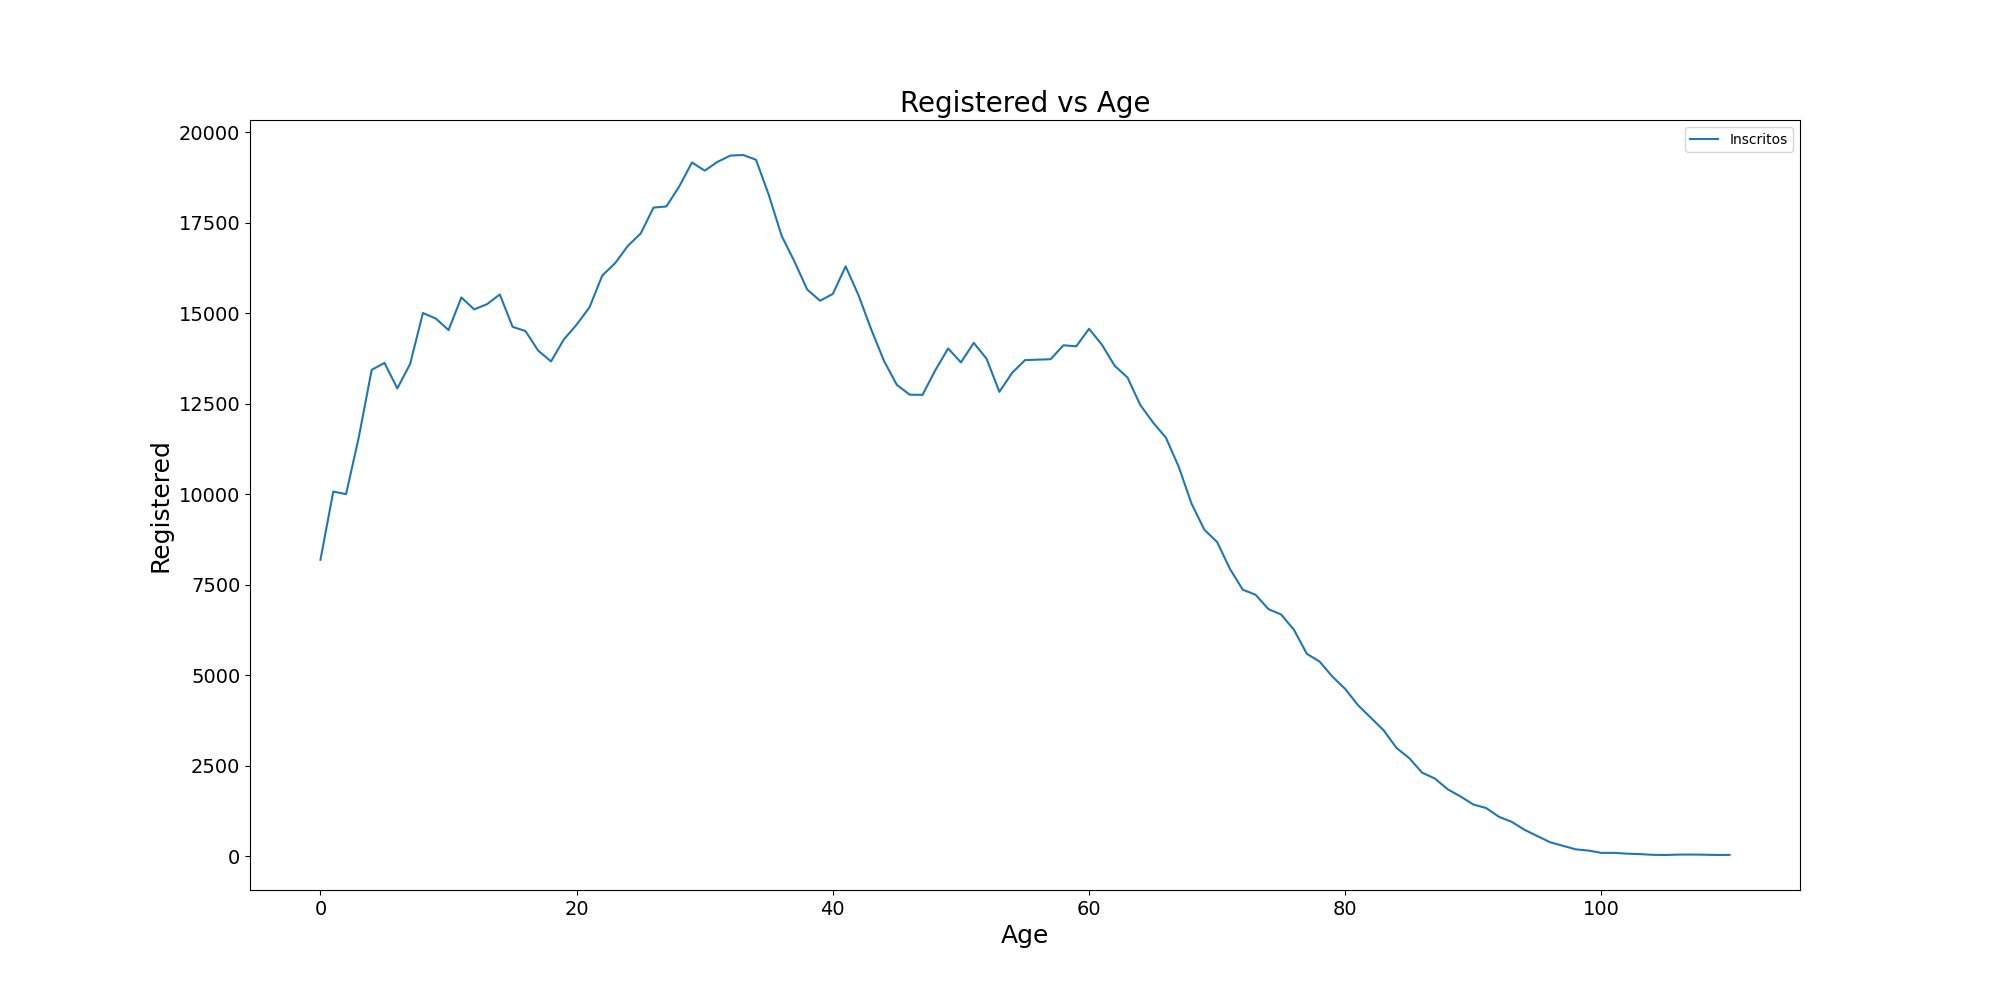
\includegraphics[width=1\textwidth]{images/4.simulation/Registered_vs_Age.png}
    \caption{Registered vs Age from SMPHS in 2023}
    \label{fig:registered_vs_age}
\end{figure}

\subsubsection*{Public Healthcare Registrations}

To sustain the population over time, new individuals must register in the public healthcare system each year. Figure \ref{fig:registered_vs_age} illustrates that many individuals are not registered at birth.

\begin{figure}[H]
    \centering
    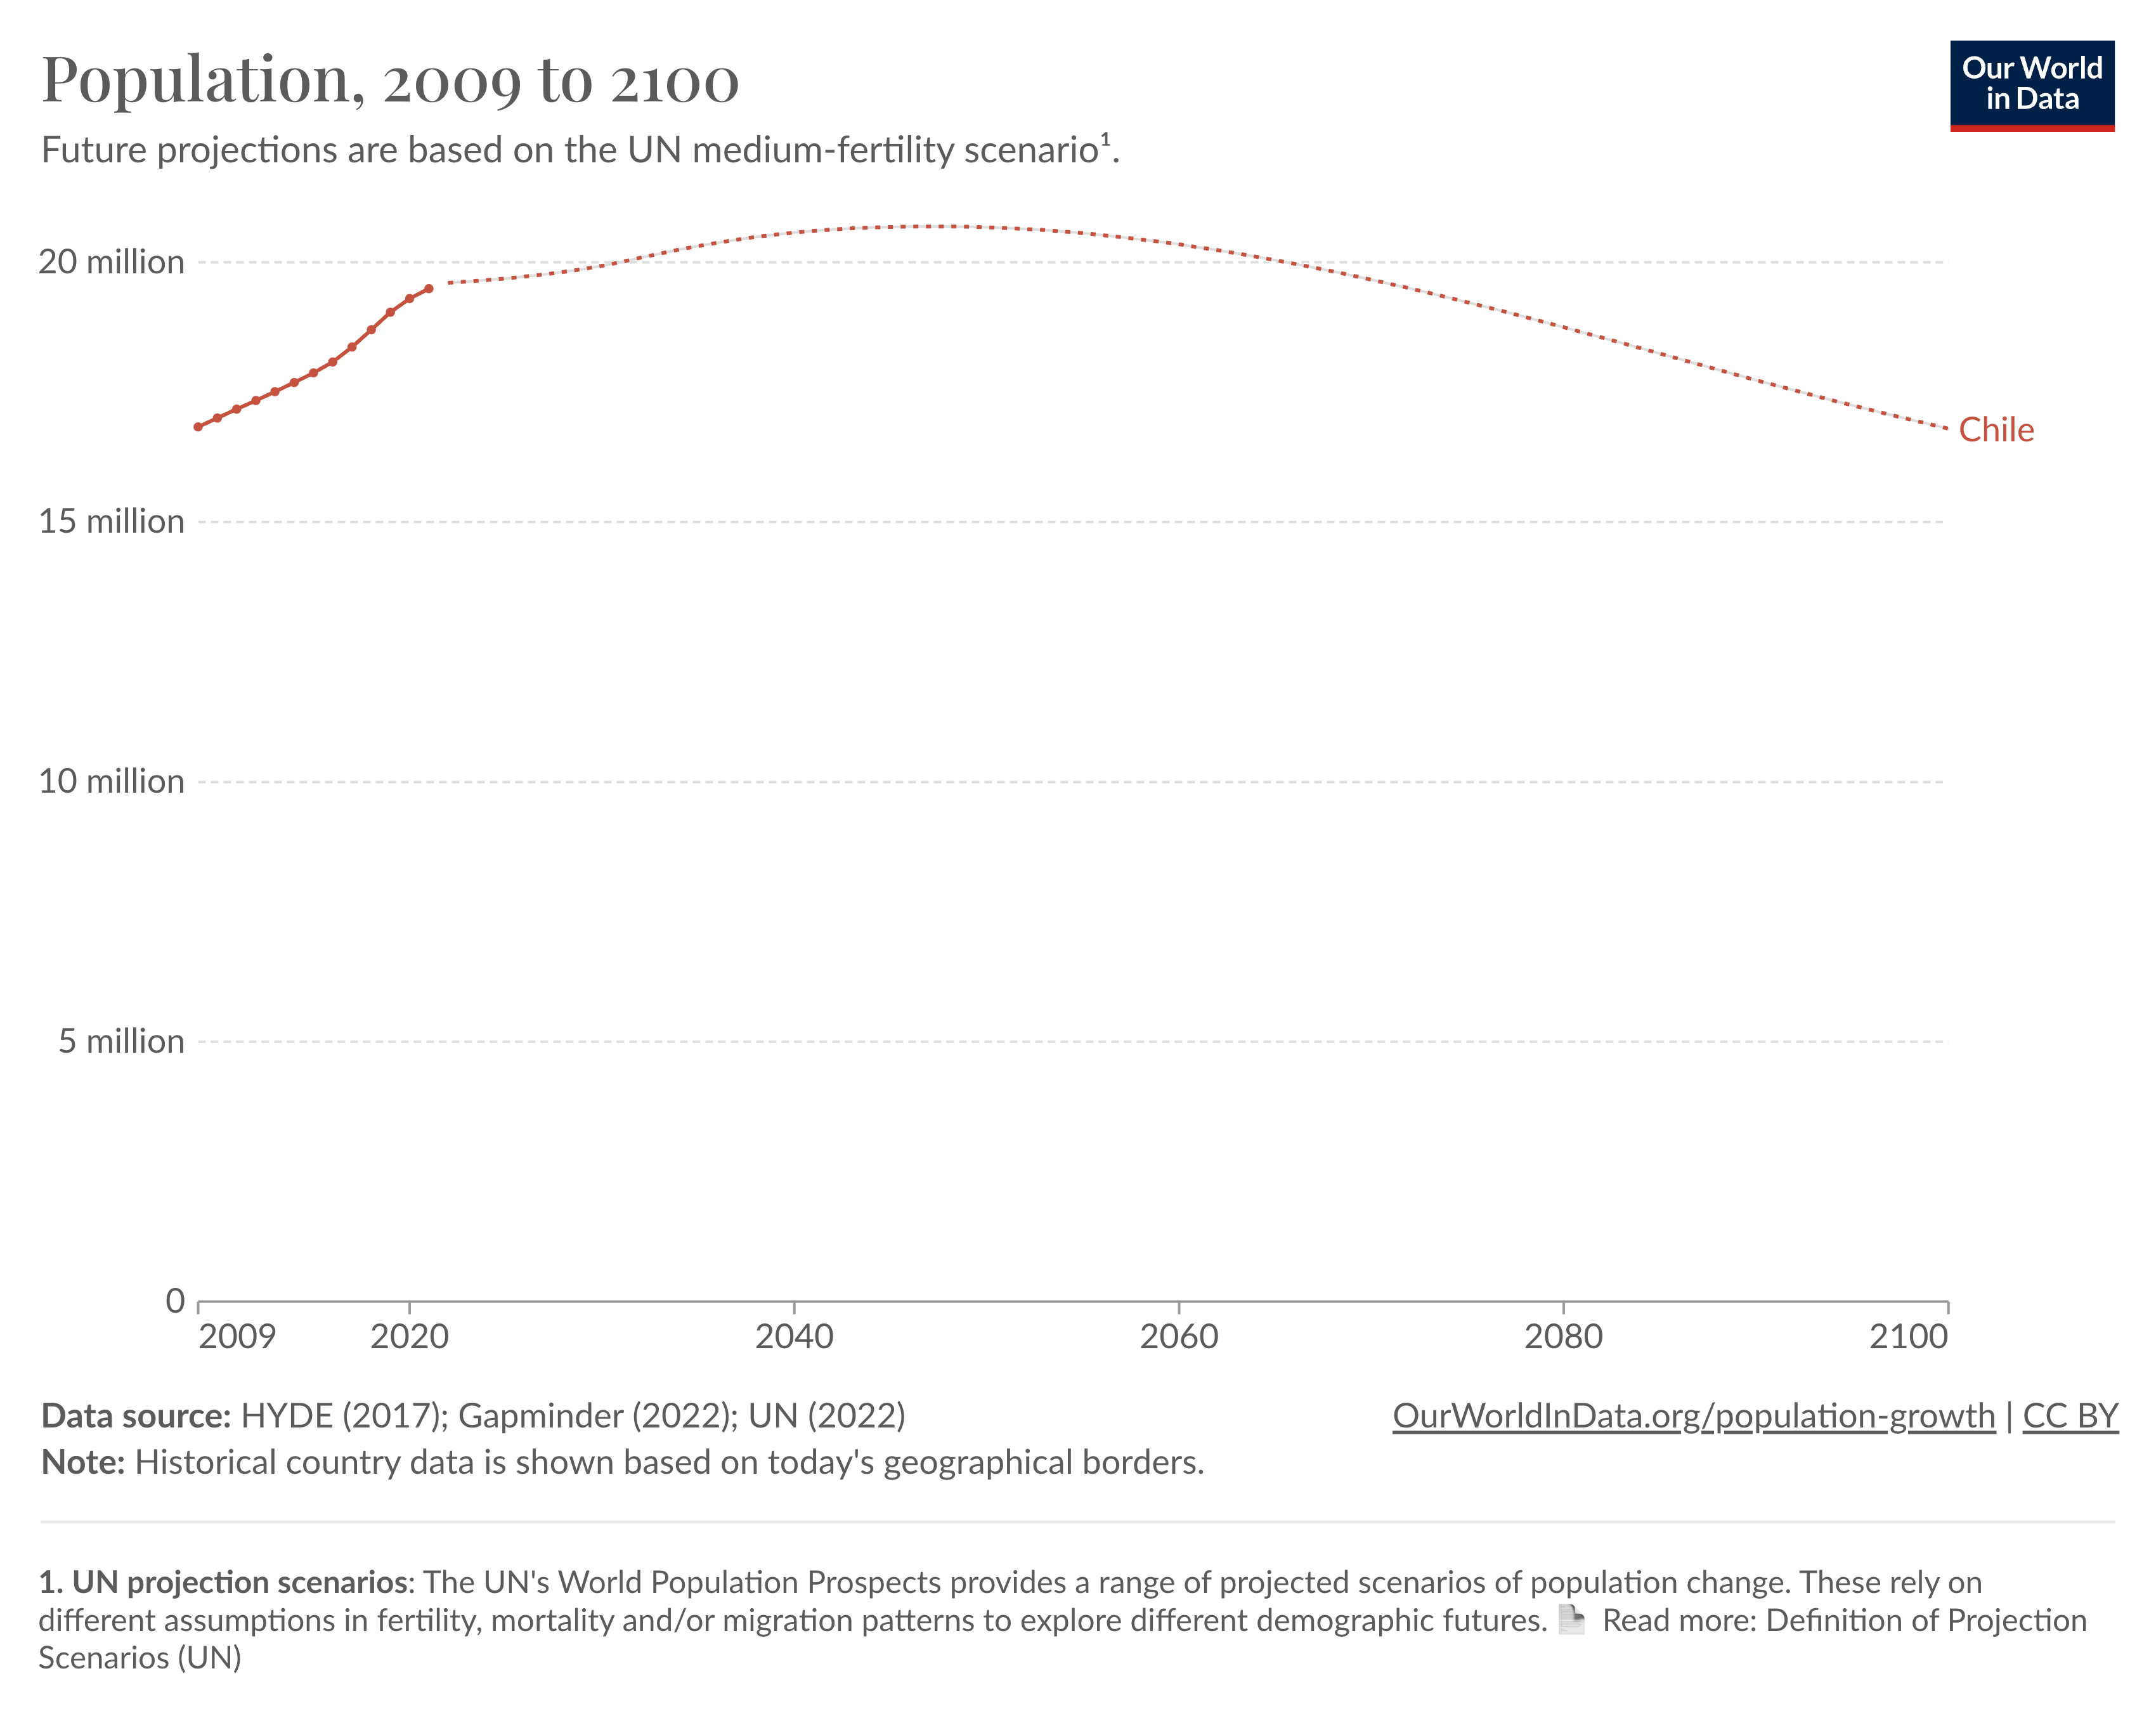
\includegraphics[width=1\textwidth]{images/4.simulation/chile_population_projection.png}
    \caption{Chilean Population Projection\textsuperscript{1}}
    \label{fig:chilean_population_projection}
\end{figure}

\footnotetext[1]{From \textit{Population Projection}. Our World on Data, 2023. \url{https://ourworldindata.org/grapher/population-long-run-with-projections?time=2009..latest&country=~CHL}}

As shown in Figure \ref{fig:chilean_population_projection}, the Chilean population is expected to grow over the next 20 years before gradually declining. Given that the growth and decline trends are neither significant nor reliable, this population trend was considered insignificant for the simulation. Therefore, the goal is to maintain a constant registered population.

\begin{table}[H]
\caption{Registrations per year in the Simulation}
\centering
\begin{tabular}{|c|c|}
\hline
Age Interval & Number of Births\\ \hline
0 & Normal(9000, 500)\\ \hline
1-8 & Normal(3200, 300)\\ \hline
21-30 & Normal(1800, 300)\\ \hline
\end{tabular}

\label{table:registrations_per_year}
\end{table}

The approach works by establishing constant birth rates, with slight random deviations, across different age intervals. This approach ensures the distribution of registered individuals remains consistent, as demonstrated in Table \ref{table:registrations_per_year}.

\subsubsection*{Cohort Life Expectancy}

To ensure accurate simulation of individual lifespans, access to cohort life expectancy data is crucial. While traditional life expectancy figures provide an average lifespan for a population, our simulation required more specific cohort-based data, detailing the average lifespan of individuals born in particular years. 

Although such data for the Chilean population was available publicly, it had limitations, covering the years 1992 to 2050 and extending to one hundred years of age \cite{noauthor_proyecciones_2024}. In contrast, the US national Social Security database offered a more comprehensive dataset, spanning from 1900 to 2095 and including both real and simulated life expectancies up to age 119. Due to its broader range and depth, the US dataset was considered more suitable for our simulation. Despite attempts to obtain extended data from the Chilean National Statistics Institute, no response was received.

Due to the extensive nature of the dataset, comprising 23,520 rows and 14 columns, detailed tables are not included in this thesis but can be accessed through the US Social Security Administration Site \cite{noauthor_social_2024}.

\begin{figure}[H]
    \centering
    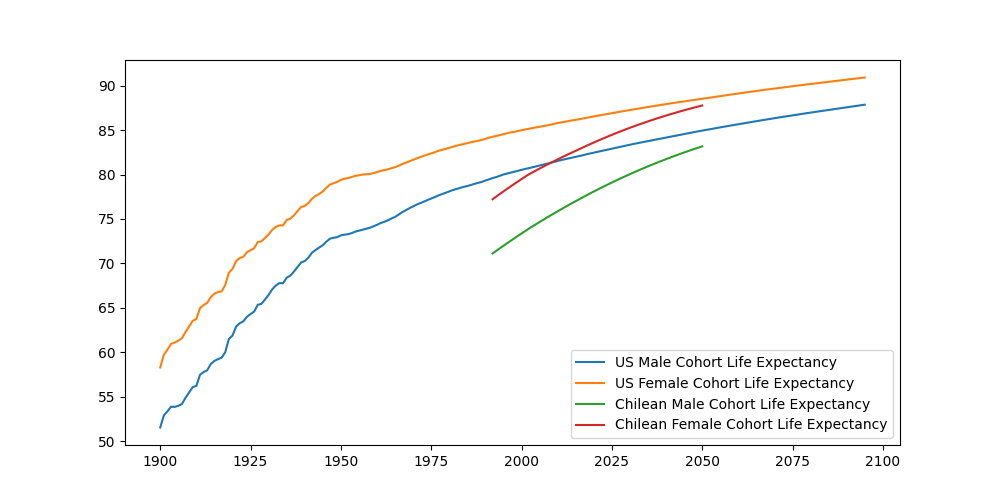
\includegraphics[width=1\textwidth]{images/4.simulation/cohort_life_expectancy.png}
    \caption{Cohort Life Expectancy}
    \label{fig:cohort_life_expectancy}
\end{figure}

Figure \ref{fig:cohort_life_expectancy} confirms the wider age range covered by the US data compared to the Chilean dataset. However, it also reveals a notable difference in life expectancy between the two populations. Although this gap may not greatly influence the simulation's results, it does raise concerns about the datasets' compatibility. This difference underscores the need to carefully review and possibly adjust other data points in the simulation to ensure they align with the unique characteristics of the Chilean population.

\subsection{CRC Disease Parameters}

All the data sources for CRC in this study are from outside Chile. This raises concerns, as the behavior of CRC can vary significantly by region. Factors like age, sex, smoking, and body mass index influence CRC incidence rates and differ across regions, as highlighted by \citeA{doubeni_contribution_2012}. Additionally, race and geographic location also impact CRC incidence, as shown by \citeA{wang_geographic_2023}. Ideally, comparable data will become available in Chile to ensure more accurate regional representation in the future.

\subsubsection*{Prevalence}

Determining whether an individual will develop colorectal cancer during their lifetime is a critical aspect of the simulation process. However, obtaining accurate data for this probability, particularly for the Chilean population, poses a challenge. While prevalence and incidence rates are commonly available, specific lifetime risk data is scarce. In Chile, the projected incidence rate stands at 20.4 cases per 100,000 inhabitants, according to the most recent data \cite{rios_situacion_2020}. Nonetheless, the most reliable indicator of lifetime risk was sourced from the United States, where it's reported as 4.4\% for men and 4.1\% for women \cite{siegel_cancer_2020}. These lifetime risk parameters are detailed in Table \ref{table:crc_lifetime_risk}.

\begin{table}[H]
\caption{Lifetime Risk of developing CRC}
\centering
\begin{tabular}{|c|c|}
\hline
Sex & Lifetime Risk\\ \hline
Male & 4.4\%\\ \hline
Female & 4.1\%\\ \hline
Average & 4.25\%\\ \hline
\end{tabular}
\label{table:crc_lifetime_risk}
\end{table}

\subsubsection*{Cancer Stage on Symptomatic or Asymptomatic Detection}

The simulation determines, when generating each individual, at which stage their cancer will be detected, either asymptomatically or symptomatically. This probability for each stage was derived from a study in the Netherlands. This study compared the stage distribution of CRC patients whose disease was detected by symptoms versus those detected by a fecal occult blood test (FOBT) screening strategy \cite{van_rossum_earlier_2009}.

\begin{figure}[H]
    \centering
    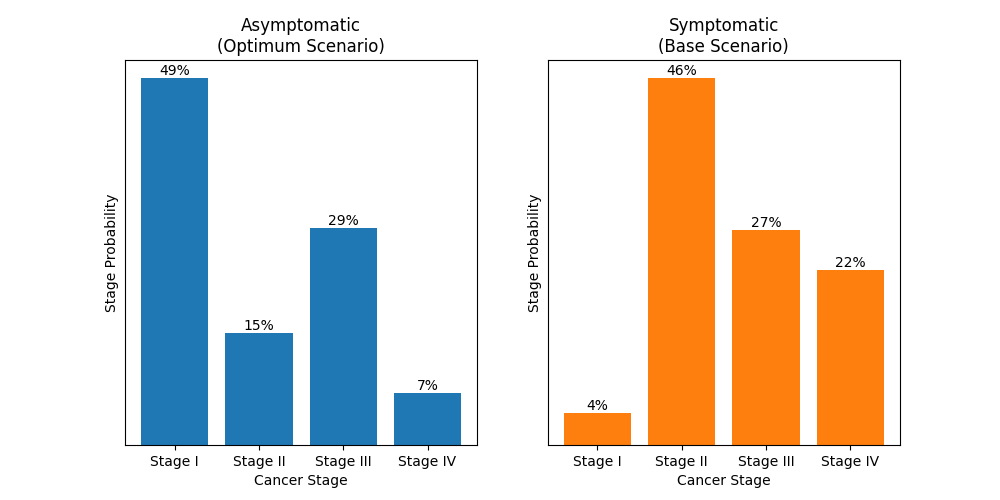
\includegraphics[width=1\textwidth]{images/4.simulation/cancer_stage_probability.png}
    \caption{Symptomatic or Asymptomatic Detection}
    \label{fig:symptomatic_vs_asymptomatic_detection}
\end{figure}

The distribution of asymptomatic and symptomatic cancer stages is illustrated in Figure \ref{fig:symptomatic_vs_asymptomatic_detection}. In the asymptomatic graph, the optimum scenario is depicted, where all detections occur without symptoms. Conversely, the base case scenario represents a situation where all detections occur due to symptoms, similar to the current state in the SMPHS.

The effectiveness of the screening strategy is reflected in the percentage of asymptomatic detections. As this percentage increases, the distribution of cancer stages will shift closer to the optimum scenario and further from the base case.

\subsubsection*{Symptomatic Age Expectancy}

The first event simulated in CRC individuals is the age at which they develop symptoms of the disease. This step requires data on CRC cases by age.

Unfortunately, the available data on CRC cases by age in Chile was insufficient and lacked the necessary detail for our simulation model. To address this limitation, we sourced the age distribution of new cases from the US Cancer Statistics site \cite{noauthor_uscs_2024}. This dataset provides a comprehensive breakdown by age group, allowing for a more detailed representation of CRC incidence. The extracted age distribution is presented in Table \ref{table:cases_by_age_group}.
\begin{table}[H]
\caption{USA CRC Cases by Age Group}
\centering
\begin{tabular}{|c|c|c|c|}
\hline
Age Group & Cases & Age Group & Cases\\ \hline
1-4       & 0     & 45-49     & 6861\\ \hline
5-9       & 18    & 50-54     & 11429\\ \hline
10-14     & 130   & 55-59     & 12564\\ \hline
15-19     & 259   & 60-64     & 15475\\ \hline
20-24     & 421   & 65-69     & 16809\\ \hline
25-29     & 731   & 70-74     & 16069\\ \hline
30-34     & 1452  & 75-79     & 13502\\ \hline
35-39     & 2471  & 80-84     & 11168\\ \hline
40-44     & 3949  & 85-120    & 12933\\ \hline
\end{tabular}
\label{table:cases_by_age_group}
\end{table}

\subsubsection*{Asymptomatic Screenable Sojourn Time}

It's crucial to simulate the period when CRC is detectable but not yet symptomatic. To address this, a study using the German National Screening Colonoscopy Database was reviewed, providing insights into the sojourn time of the preclinical stage of CRC \cite{brenner_sojourn_2011}. The study detailed age groups and sojourn times by sex, as outlined in Table \ref{table:asymptomatic_sojourn_time}.

\begin{table}[H]
\caption{CRC Asymptomatic Screenable Sojourn Time}
\centering
\begin{tabular}{|c|c|c|}
\hline
Age Group & Male Sojourn Time (95\% CI) & Female Sojourn Time (95\% CI) \\ \hline
0-59   & 5.5 (5.1, 6.0) & 4.7 (4.3, 5.1)\\ \hline
60-64  & 5.2 (4.9, 5.5) & 4.5 (4.1, 4.8)\\ \hline
65-69  & 4.7 (4.5, 4.9) & 4.6 (4.3, 4.8)\\ \hline
70-74  & 4.9 (4.6, 5.1) & 4.8 (4.5, 5.1)\\ \hline
75-79  & 5.0 (4.7, 5.3) & 5.2 (4.8, 5.6)\\ \hline
80-120 & 5.5 (5.0, 6.0) & 5.8 (5.3, 6.3)\\ \hline
\end{tabular}
\label{table:asymptomatic_sojourn_time}
\end{table}

\subsubsection*{CRC Life Expectancy}

It's necessary to simulate the years from the symptomatic detection until the passing of the individual. We used data from a study from the Netherlands which has the life expectancy of CRC patients depending on the stage and the age it was detected \cite{soerjomataram_most_2012}. 

\begin{table}[H]
\caption{CRC Life Expectancy by Sex and Stage}
\centering
\begin{tabular}{|c|c|c|}
\hline
Stage \& Age & Male & Female\\ \hline
I   & 25.3 & 29.8 \\ \hline
II  & 19.2 & 20.9 \\ \hline
III & 13.6 & 16.8 \\ \hline
IV  & 2.1  & 2.2  \\ \hline
\end{tabular}
\label{table:crc_life_expectancy_by_stage}
\end{table}

\begin{table}[H]
\caption{CRC Life Expectancy by Sex and Age}
\centering
\begin{tabular}{|c|c|c|}
\hline
Age & Male & Female\\ \hline
50  & 12.3 & 13.3 \\ \hline
65  & 9.4  & 11.5 \\ \hline
80  & 5.5  & 7    \\ \hline
\end{tabular}
\label{table:crc_life_expectancy_by_age}
\end{table}

The data provided in Tables \ref{table:crc_life_expectancy_by_stage} and \ref{table:crc_life_expectancy_by_age} were utilized to formulate a function capable of determining life expectancy based on both the stage of CRC and the individual's age. This function was developed through interpolation, calculating life expectancy for ages ranging from 1 to 120 years. To achieve this, the stage and age parameters were averaged using dynamically assigned weights. At birth (0 years old), the stage weight is set at 20\%, incrementing linearly until reaching 100\% at 120 years old. The resulting life expectancies generated by this function are graphically depicted in Figures \ref{fig:crc_male_life_expectancies} and \ref{fig:crc_female_life_expectancies}.

\begin{figure}[H]
    \centering
    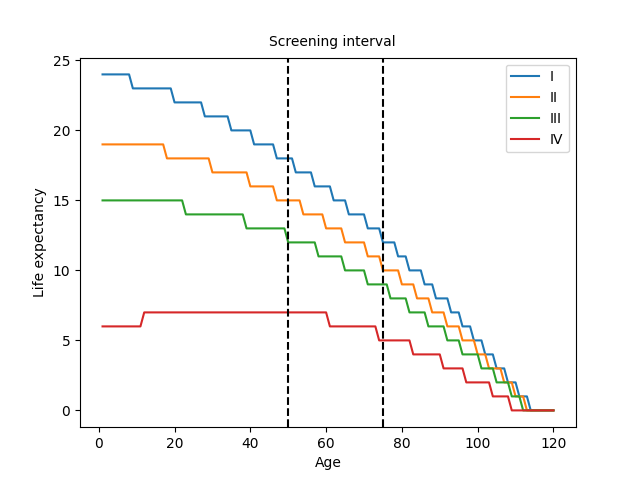
\includegraphics[width=1\textwidth]{images/4.simulation/crc_male_life_expectancies.png}
    \caption{Male CRC Life Expectancies by Age and Stage}
    \label{fig:crc_male_life_expectancies}
\end{figure}

\begin{figure}[H]
    \centering
    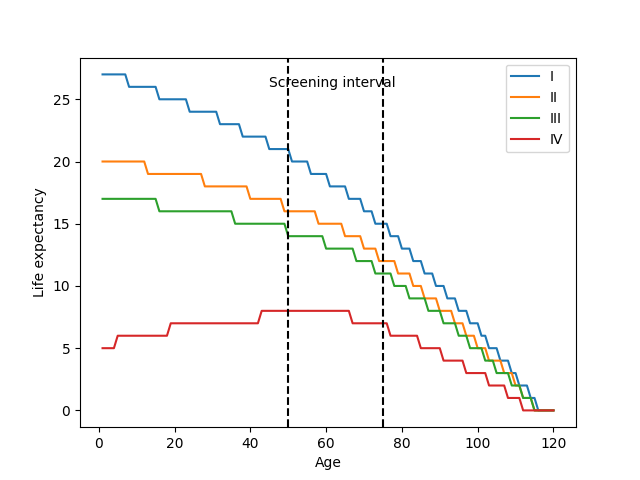
\includegraphics[width=1\textwidth]{images/4.simulation/crc_female_life_expectancies.png}
    \caption{Female CRC Life Expectancies by Age and Stage}
    \label{fig:crc_female_life_expectancies}
\end{figure}

When colorectal cancer is detected while still asymptomatic, the patient's expected age of death is recalculated based on the asymptomatic stage. This adjustment accounts for any difference in years between the original prognosis and the recalculated age, contributing to the overall "years gained" statistic. 

Although this recalibration occasionally results in progression to a more advanced stage, such instances are rare. Moreover, across a wide range of cases analyzed, the cumulative years gained through this strategy consistently show positive outcomes in the long term.

\subsubsection*{Screening Exam}

It was decided that the screening test had to be a fecal immunochemical test (FIT) as it shows better performance compared to the fecal occult blood test (FOBT) \cite{zhu_comparison_2010} in every exam indicator.

This test is being offered by the private sector UC Christus clinic network which has the FIT exam in three variants, with one, two and three samples. As the two and three-sample tests have twice and thrice the value of the single sample test, and the performance indicators don’t seem to improve with more than one sample \cite{amitay_fecal_2019}, the one sample test is the exam chosen for this strategy.

For the tests sensitivity and specificity we used a study that did a Systematic Review and Meta-analysis of many FIT studies \cite{lee_accuracy_2014} which found the values of performance characteristics presented in Table \ref{table:fit_performance_characteristics}.

\begin{table}[H]
\caption{FIT Performance Characteristics}
\centering
\begin{tabular}{|c|c|}
\hline
Performance Characteristic & Value (95\% CI)\\ \hline
Sensitivity & 0.79 (0.69, 0.86)\\ \hline
Specificity & 0.94 (0.92, 0.95)\\ \hline
\end{tabular}
\label{table:fit_performance_characteristics}
\end{table}

\subsubsection*{Adherence to Screening Strategy}

Adherence to screening strategies significantly impacts their effectiveness. Various countries, primarily in Europe, have implemented similar screening approaches, each with different levels of adherence and outcomes \cite{navarro_colorectal_2017}.

\begin{table}[H]
\caption{Countries Screening Strategy Adherences}
\centering
\begin{tabular}{|c|c|c|c|}
\hline
Country     & Adherence & Country & Adherence\\ \hline
Canada         & 16.1\% & California (USA)& 48.2\% \\ \hline
Croatia        & 19.9\% & Ireland         & 51\%   \\ \hline
South Korea    & 21\%   & England         & 52\%   \\ \hline
Taiwan         & 21.4\% & Italy           & 54.4\% \\ \hline
Czech Republic & 22.7\% & Slovenia        & 60.43\%\\ \hline
France         & 36.1\% & Thailand        & 62.9\% \\ \hline
Australia      & 45.4\% & Netherlands     & 68.2\% \\ \hline
Lithuania      & 46\%   &  &  \\ \hline
\end{tabular}
\label{table:countries_adherence_percentage}
\end{table}

As depicted in Table \ref{table:countries_adherence_percentage}, adherence rates for CRC screening vary significantly across different countries, typically falling within the range of 20\% to 60\%. For the simulation in this study, eight adherence scenarios were selected. Taking a cautious approach, an initial adherence rate of 20\% was chosen, reflecting the limited experience of the Chilean government and healthcare system in implementing preventive medicine programs. The first five scenarios represent the incremental introduction of the screening strategy at adherence rates of 0\%, 5\%, 10\%, 15\%, and 20\%. Additionally, the remaining three scenarios project potential future adherence rates of 40\%, 60\%, and 80\%. They are presented in Table \ref{table:simulation_adherence_percentage_scenarios}.

\begin{table}[H]
\caption{Simulation Adherence Percentage Scenarios}
\centering
\begin{tabular}{|c|c|c|c|}
\hline
Scenario & Adherence & Scenario & Adherence\\ \hline
1  & 0\%  & 5 & 20\% \\ \hline
2  & 5\%  & 6 & 40\% \\ \hline
3  & 10\% & 7 & 60\% \\ \hline
4  & 15\% & 8 & 80\% \\ \hline
\end{tabular}
\label{table:simulation_adherence_percentage_scenarios}
\end{table}

\subsection{Procedures Costs}

\subsubsection*{Screening Test}

The national FIT screening cost, crucial for our analysis, was exclusively available in the 2020 UC Christus examination fees. At a rate of 5,865 Chilean pesos (CLP), roughly equivalent to six US dollars, this data served as our sole reference point for determining the cost parameter.

\subsubsection*{Colonoscopy Exam}

Given the significance of this parameter in the simulation, we aimed to reduce bias in two ways. First, by considering prices from different clinics, and second, by using actual price values rather than lower estimated costs to maintain an objective perspective in the model's construction.

The lowest price that was obtained from the government's GES system, which was found to be 80,560 CLP. However, this price is not representative of the market, as most private clinics charge between 250,000 and 450,000 CLP. Private clinics typically break down their prices into two components: medical fees (MF) and other expenses (OE).

For a premium experience, we looked at the price from Clinica Alemana, one of Santiago's top clinics, which totaled \$504,205 (\$274,096 for MF and \$230,109 for OE), representing a high-end price point.

A mid-tier option was sourced from UC Christus clinics, with a price of \$425,621 (\$330,752 MF + \$94,869 OE). Similarly, Clinica Bupa, another mid-tier clinic, offered a competitive price of \$333,190 (\$135,920 MF + \$197,270 OE), falling within the mid-range of prices.

All of these sources, along with their respective averages, are detailed in Table \ref{table:colonoscopy_prices}.

\begin{table}[H]
\caption{Colonoscopy Prices}
\centering
\begin{tabular}{|c|c|}
\hline
Hospital & Colonoscopy Price\\ \hline
Clínica Alemana & \$504 205\\ \hline
UC Christus     & \$425 621\\ \hline
Clínica Bupa    & \$333 190\\ \hline
Average         & \$421 005\\ \hline
\end{tabular}
\label{table:colonoscopy_prices}
\end{table}




\subsubsection*{Treatment by CRC Stage}

Treatment cost is a crucial parameter in the simulation, as it directly impacts resource allocation in the Screening and Confirmation stages. Higher costs for advanced stages of the disease incentivize early detection. Unfortunately, no data on CRC treatment costs by stage was available for Chile. To address this, a study from the Basque public health system in 2017 was used as a proxy. The MND team validated the obtained values as reasonable.

The Basque study's costs were initially converted to Chilean pesos based on the Euro's value at that time and then adjusted for inflation to 2023. These adjusted figures are detailed in Table \ref{table:crc_cost_by_stage}.d

\begin{table}[H]
\caption{CRC Cost by Stage}
\centering
\begin{tabular}{|c|c|}
\hline
Stage & Cost\\ \hline
I     & \$ 7 647 243\\ \hline
II    & \$11 293 220\\ \hline
III   & \$11 567 473\\ \hline
IV    & \$45 414 136\\ \hline
\end{tabular}
\label{table:crc_cost_by_stage}
\end{table}

\section{Limitations and Challenges}
\label{sec:limitation_and_challenges}

The limitations and challenges segment illuminates the constraints and future improvements that are currently involved the simulation model. Despite efforts to develop comprehensive and accurate models, certain limitations and challenges persist, ranging from data availability and quality to model assumptions and simplifications. Identifying and addressing these limitations and challenges promotes continuous improvement in simulation methodologies and enhances the credibility of the simulation.

\subsection*{Simulation Model Validations}
Validating a simulation model is crucial for establishing its credibility as a reliable tool for healthcare planning. In our study, we did not strictly adhere to any of the validation techniques. While some external validation was conducted by the MND team and medical advisors, it was not performed according to a formal methodology recognized as official validation.

The study by \citeA{smith_simulation_2020} went beyond simply categorizing CRC screening simulation models; it also assessed them against five model validation techniques. Interestingly, none of the models reported all five techniques, and a significant 58\% reported none. These techniques are outlined in detail in a publication by \citeA{eddy_model_2012}. 

It is essential for this simulation model to undergo validation using a rigorous methodology. Addressing this is one of the primary challenges that must be addressed to enhance the model's quality and reliability.

\subsection*{Considerations for CRC Modeling}

Modeling the disease progression of CRC is a complex task. The diagnostic and treatment pathways need to be simplified, leading to the omission of some details of the actual process. Additionally, the quality of the data used in every aspect must be assessed, as it significantly impacts the validity of the outcomes.

For instance, the time frames used for the progression of CRC in the simulation are a simplification of the actual cancer progression. The earliest stage of tumors, the polyps, were not addressed in the simulation model.

Another simplification is seen in the adherence aspect, which was represented as a probability of individuals undergoing the entire screening process in their lifetime or not participating at all. This does not accurately mirror common behaviors regarding preventive medicine.

Furthermore, many parameters in the model were based on data from populations with different characteristics than those of the SMPHS. Factors such as life expectancy, CRC prevalence, CRC stage distribution, and others may vary among populations.

These limitations need to be taken into consideration when evaluating the accuracy and applicability of the current model.

\subsection*{Utilizing Specific Cost Data in Healthcare Economics}

Utilizing cost data from specific sources presents certain limitations that must be acknowledged when conducting healthcare economic analyses. 

Initially, cost data obtained from individual healthcare facilities or insurance providers may not be representative of broader healthcare system costs, as they may vary significantly depending on factors such as geographic location, patient population demographics, and institutional practices. 

Additionally, relying on data from a limited number of sources can introduce bias and inaccuracies. Such data might not fully encompass all costs related to a healthcare intervention or disease management strategy. Additionally, cost data from specific sources may lack transparency or standardization, making it challenging to compare findings across studies or extrapolate results to different healthcare settings. 

Finally, changes in healthcare reimbursement policies, technology advancements, and healthcare delivery models over time may render cost data outdated or less applicable to current healthcare contexts.


\chapter[Results]{Results}
\label{chapter:results}
This chapter examines the simulation outcomes, with a focus on key parameters influencing the results. It begins by explaining the graphs used in the analysis. Subsequently, it presents the results obtained with the default parameters and analyzes replicas of the default scenario. The sensitivity analysis follows, investigating how variations in variables such as screening frequency, screening intervals, colonoscopy costs, and FIT performance indicators impact the results. This thorough exploration provides stakeholders with insights into the factors shaping the outcomes, assisting in evidence-based decision-making and policy formulation for optimizing colorectal cancer screening and management.

\section{Results Example}
First, we will examine the graphs used in the results to better explain their significance to the analysis.

\subsection*{Treatments Bar Chart}

This bar chart illustrates the distribution of treatments by stage.

\begin{figure}[H]
    \centering
    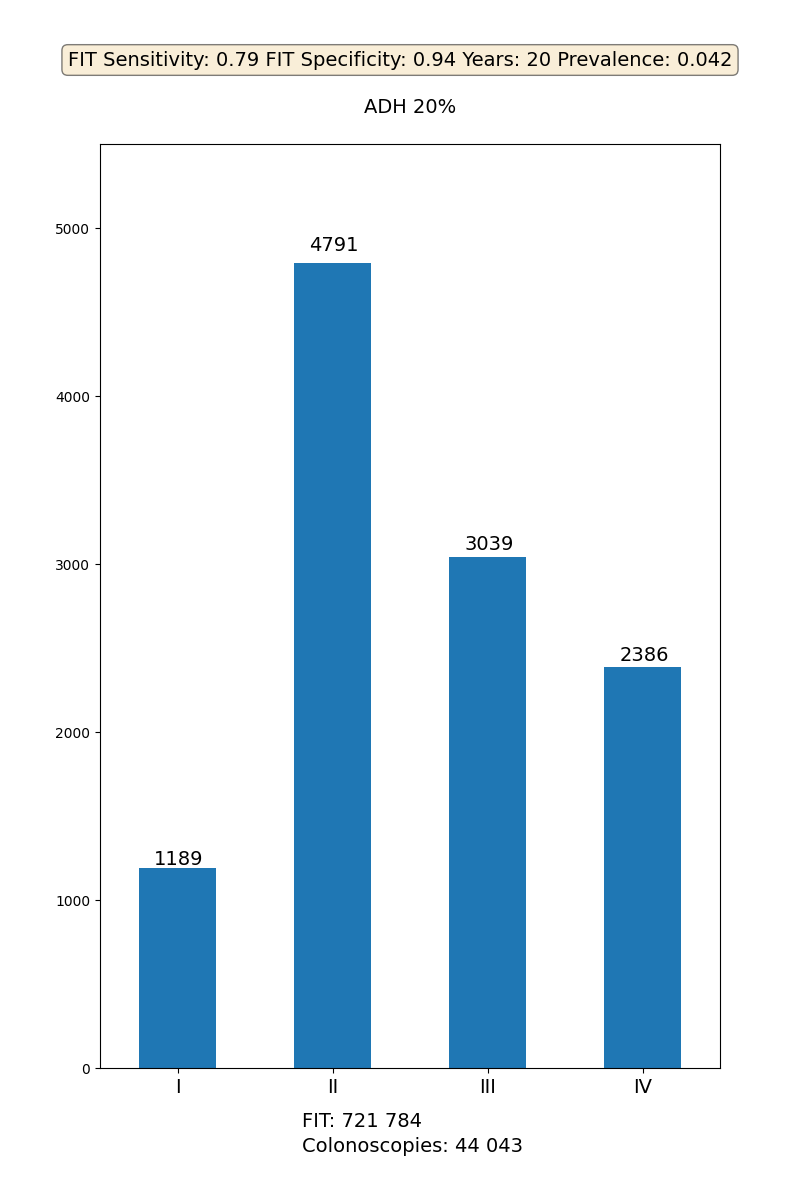
\includegraphics[scale= 0.45]{images/5.results/treatments_for_example.png}
    \caption{Example of Treatments Bar Chart}
    \label{fig:treatments_for_example}
\end{figure}

In Figure \ref{fig:treatments_for_example}, the simulation presents a single scenario, labeled "ADH 20\%" to indicate the population's adherence percentage. The yellow box displays the fixed parameters for all scenarios, while below the plot, the numbers of FIT exams and Colonoscopies performed are provided. This chart is essential for illustrating the changes in the distribution of treatment stages and the number of FIT exams and Colonoscopies performed under different scenarios.

\subsection*{Screening Efficacy Bar Chart}

This horizontal bar chart demonstrates the efficiency of the screening in detecting CRC cases during their asymptomatic period.

\begin{figure}[H]
    \centering
    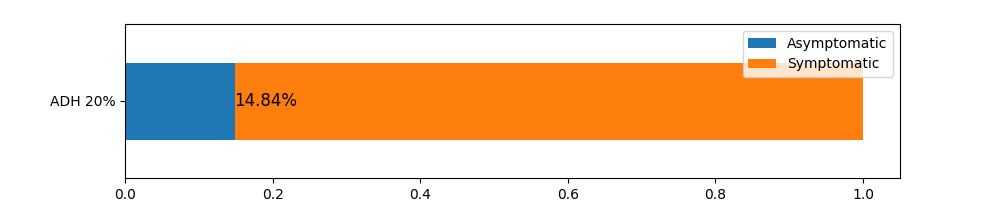
\includegraphics[scale= 0.5]{images/5.results/screening_efficacy_for_example.png}
    \caption{Example of Screening Efficacy Bar Chart}
    \label{fig:screening_efficacy_for_example}
\end{figure}

In the chart illustrated in Figure \ref{fig:screening_efficacy_for_example}, we observe the same 20\% adherence case, showing the percentage of asymptomatic treatments. This chart is valuable for comparing different scenarios and understanding how the screening strategy's effectiveness varies between them.

\begin{figure}[H]
    \centering
    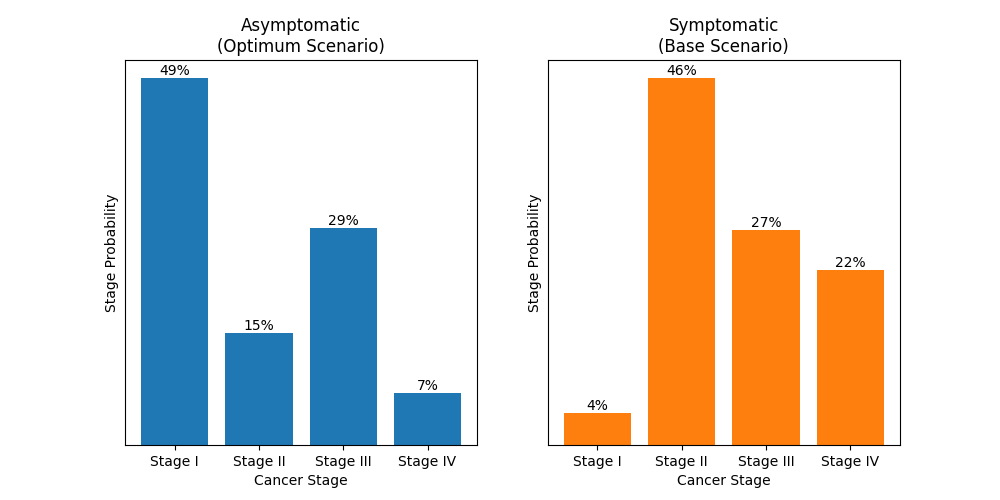
\includegraphics[width=1\textwidth]{images/4.simulation/cancer_stage_probability.png}
    \caption{Symptomatic or Asymptomatic Detection}
    \label{fig:symptomatic_vs_asymptomatic_detection_2}
\end{figure}

As depicted in Figure \ref{fig:screening_efficacy_for_example}, at 20\% adherence, approximately 15\% of all cases are treated before showing any symptoms. This implies that three out of every twenty CRC cases would align with the optimum scenario in terms of cancer stage distribution probabilities, while the remaining cases would align with the base scenario shown in Figure \ref{fig:symptomatic_vs_asymptomatic_detection_2}.

\subsection*{Costs Pie Chart}

This pie chart depicts the distribution of costs for screening and treatment procedures.

\begin{figure}[H]
    \centering
    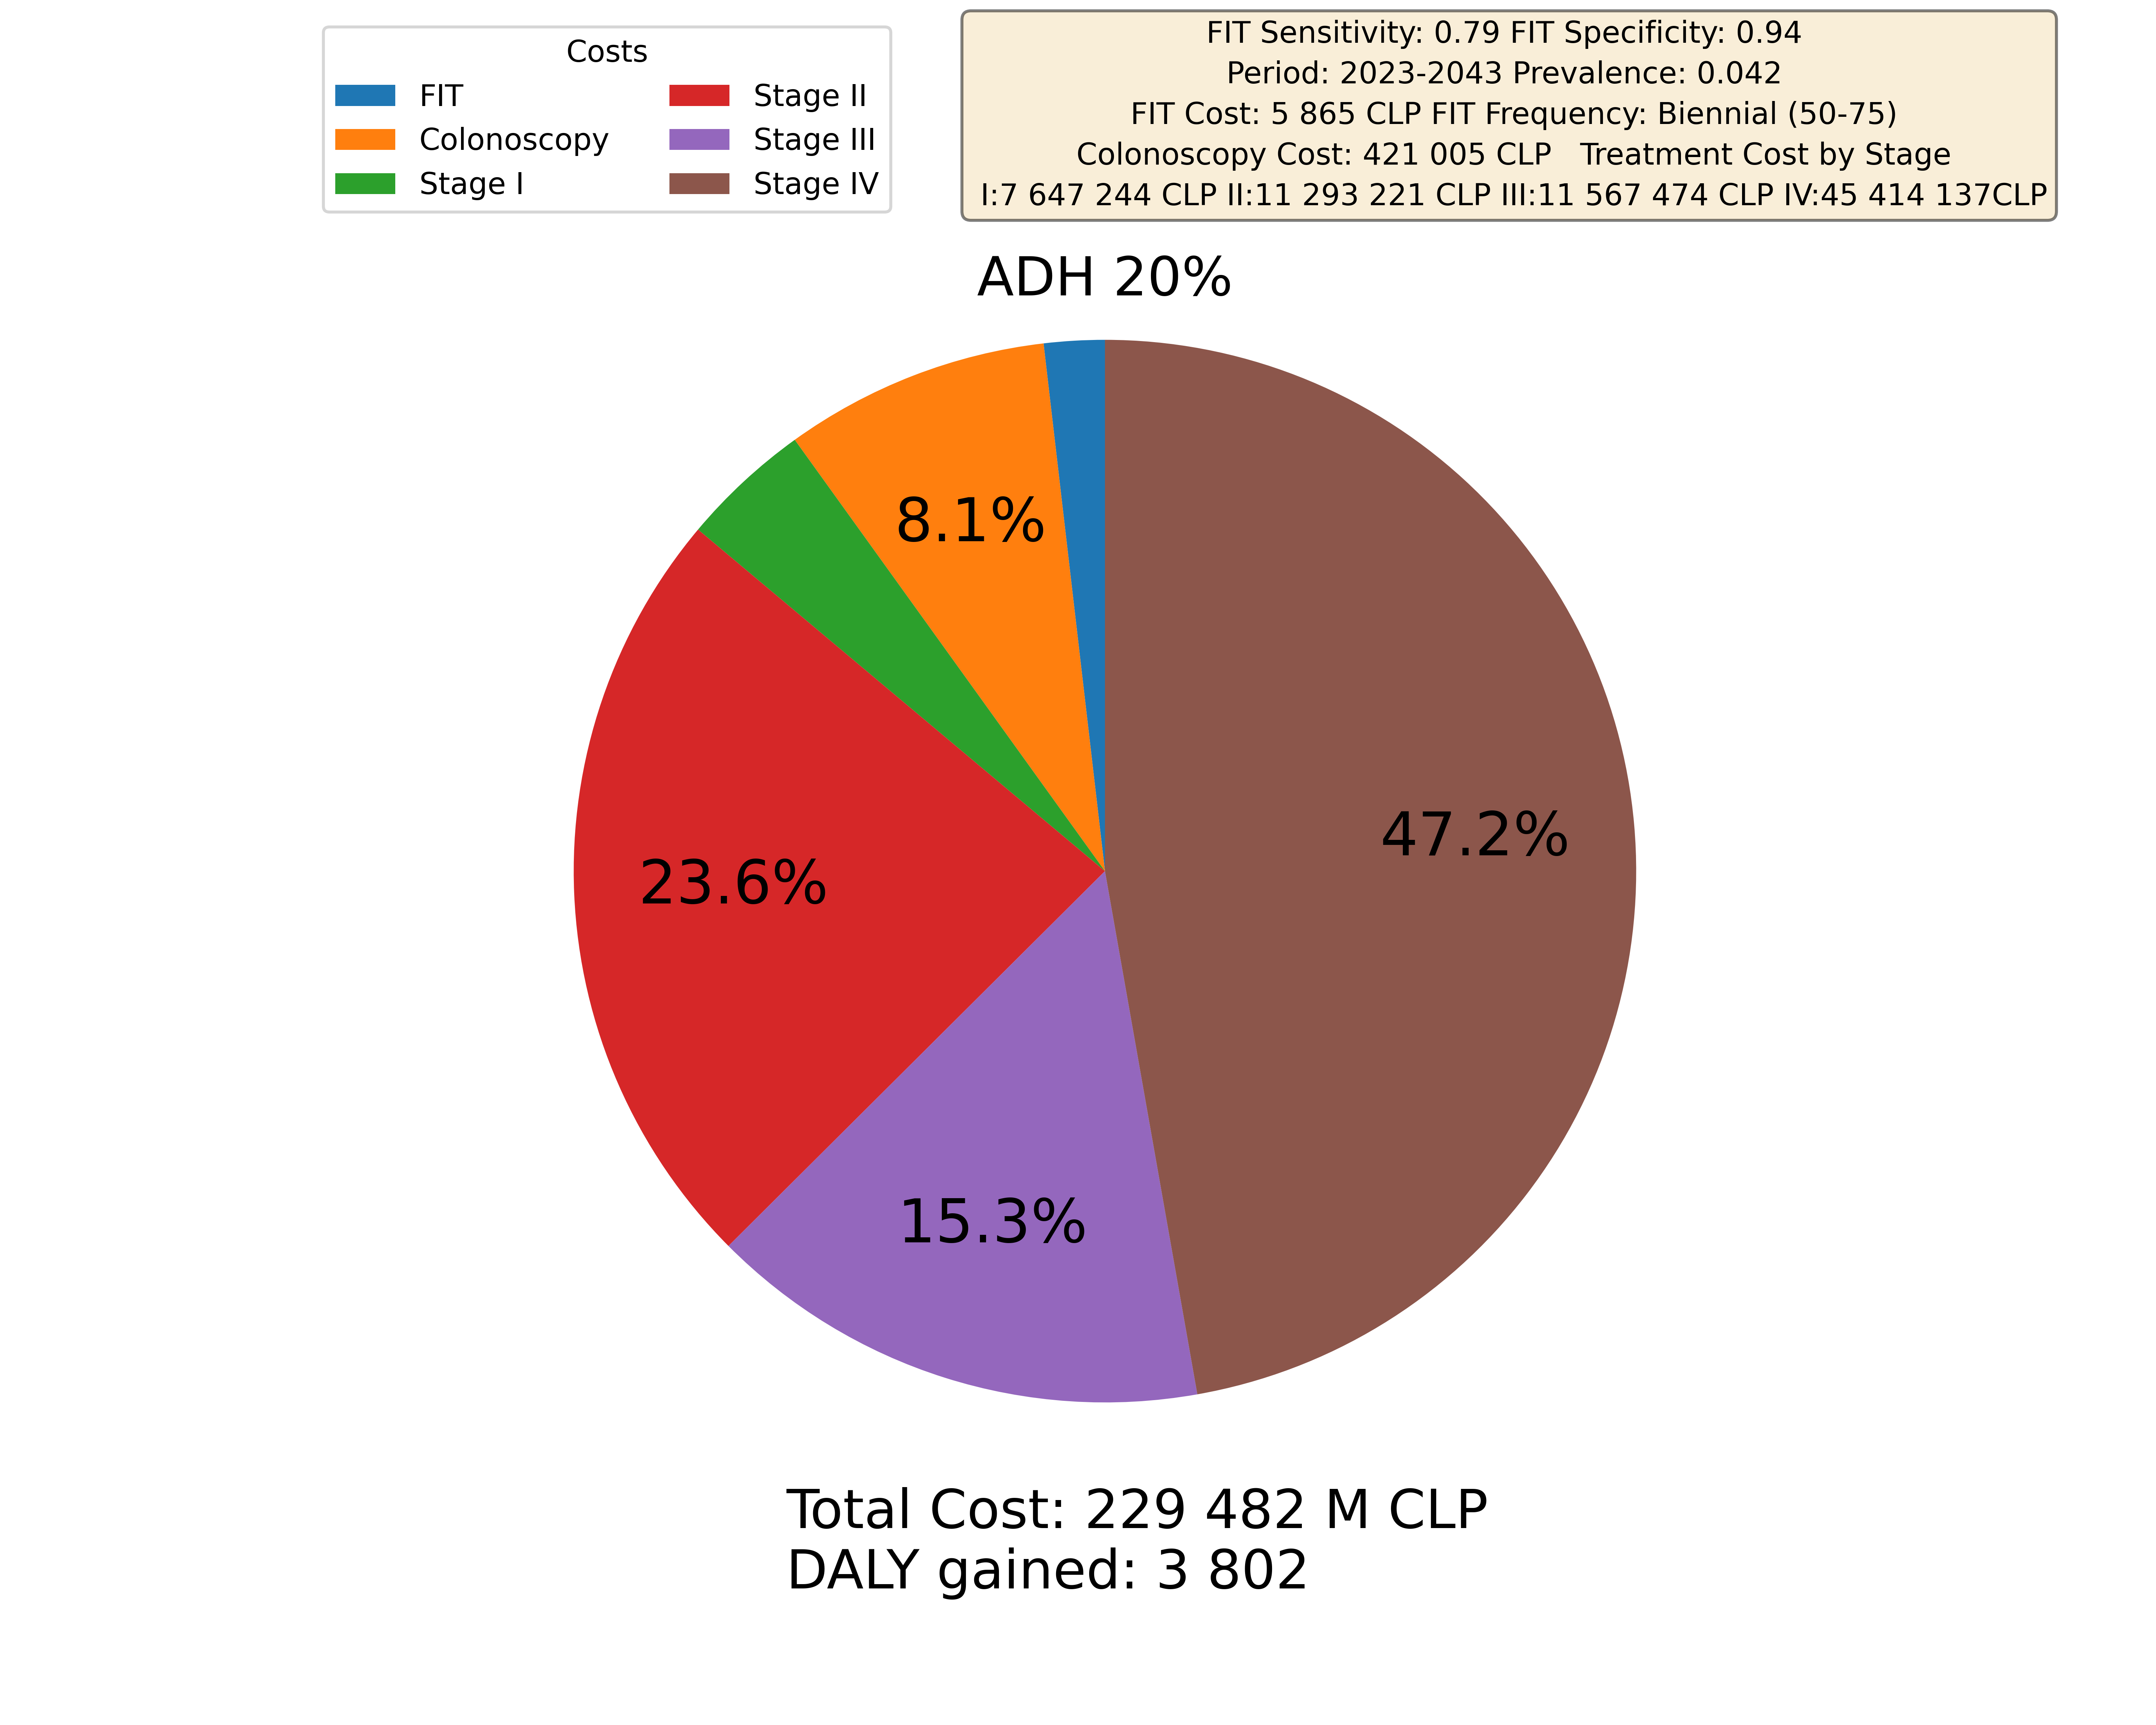
\includegraphics[scale=0.5]{images/5.results/costs_for_example.png}
    \caption{Example of Costs Pie Chart}
    \label{fig:costs_for_example}
\end{figure}

In the pie chart shown in Figure \ref{fig:costs_for_example}, we can see the six costs that constitute the CRC care process in the simulation model. The total cost and the disability adjusted life-years (DALY) gained from the screening strategy are presented below the graph. Additionally, when multiple scenarios are presented, the cost percentage difference from the base model is included. This graph serves as the primary visual support for the economic analysis of the various scenarios.

\section{Simulation Benchmarks}

The simulation results were generated using a MacBook Air with an M1 chip. The duration of each simulation varied based on the number of adherence scenarios and years simulated.

For the default simulation, which included 8 adherence scenarios, each running for 20 years, the first scenario completed in 24 seconds. In total, all 8 scenarios took 192 seconds to run. When the same 8 scenarios were simulated for 200 years, the first scenario took 257 seconds to complete, and all scenarios finished in 37 minutes.

\section{Result with the Default Parameters}

In this section, we will present the results using the default parameters. All of them where carefully described along with their sources in the \hyperref[section:simulation_parameters]{Simulation Parameters section}.

\subsection*{Effectiveness Analysis}

Assessing results independently of costs is crucial for evaluating the effectiveness of the screening strategy on CRC prognosis. This analysis allows researchers to understand the true impact of the screening approach on disease management, free from financial considerations.

\begin{figure}[H]
    \centering
    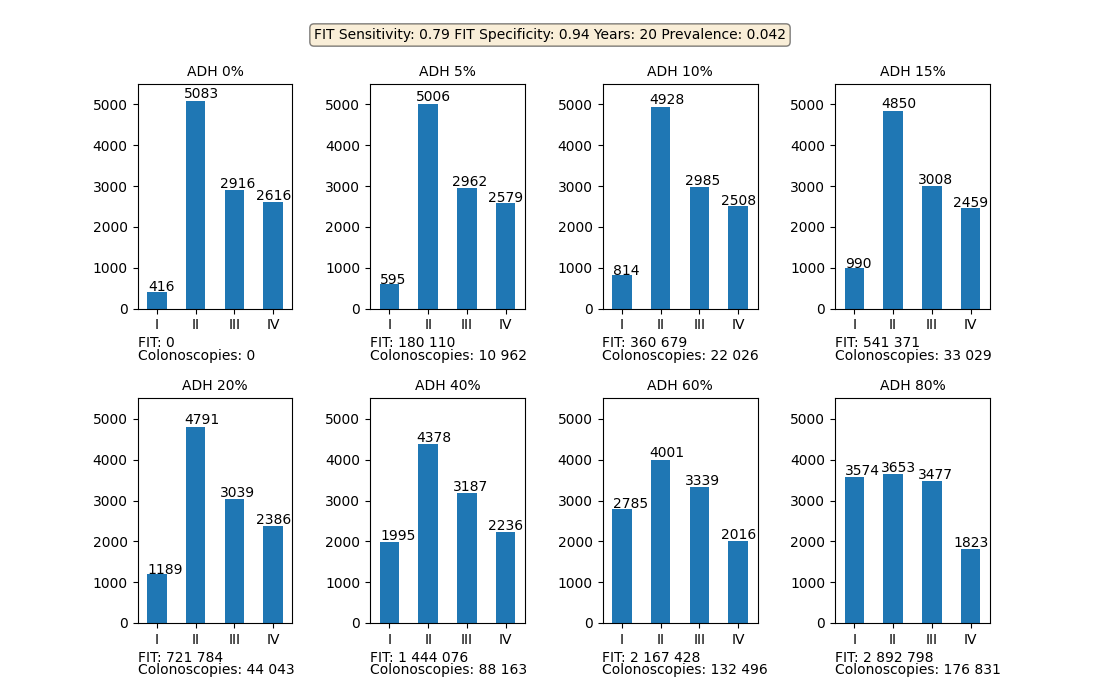
\includegraphics[width=1\textwidth]{images/5.results/treatments_by_adherence.png}
    \caption{Treatments by Adherence}
    \label{fig:treatments_by_adherence}
\end{figure}

The scenarios depicted in Figure \ref{fig:treatments_by_adherence} demonstrate a trend where higher screening adherence is associated with earlier stage treatment of cancer. At 0\% adherence, treatment primarily targets stage II, with a notable volume in stage III. As adherence increases to 5\%, 10\%, and 15\%, there is a decline in treatments for advanced stages III and IV, coupled with an increase in early-stage interventions. This trend continues at 40\%, 60\%, and peaks at 80\% adherence.

At 20\% adherence, a level that could be reasonably expected from the population in the SMPHS, there is a significant increase in resource allocation for screening exams. Approximately 36,089 FIT exams and 2,202 colonoscopies would be required annually for screening purposes alone.

\begin{figure}[H]
    \centering
    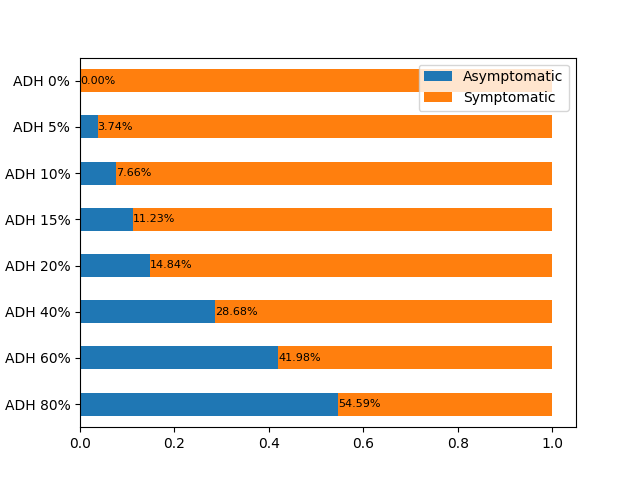
\includegraphics[width=1\textwidth]{images/5.results/screening_efficacy_by_adherence.png}
    \caption{Screening Efficacy by Adherence}
    \label{fig:screening_efficacy_by_adherence}
\end{figure}

Here, Figure \ref{fig:screening_efficacy_by_adherence} also illustrates that as adherence increases, there's a noticeable rise in asymptomatic cancer treatments, indicating earlier detection. At a population adherence of 20\%, approximately 14.8\% of all cases would be discovered during the asymptomatic period.

Graphs \ref{fig:treatments_by_adherence} and \ref{fig:screening_efficacy_by_adherence} underscore the idea that higher adherence to colorectal cancer screening leads to a shift toward earlier-stage treatment. This shift highlights the need for increased resource allocation, meaning the need for additional personnel and equipment to implement a succesful screening strategy.

\subsection*{Cost Analysis}

While the screening strategy has proven successful in improving the outcomes of earlier stage detection, it's crucial to incorporate costs into the analysis of implementation. This consideration enables decision-makers to evaluate the financial feasibility and sustainability of screening programs, ensuring the efficient allocation of resources.

\begin{figure}[H]
    \centering
    
\includegraphics[width=1\textwidth]{images/5.results/costs_by_adherence.png}
    \caption{Costs by Adherence}
    \label{fig:costs_by_adherence}
\end{figure}

The data in Figure \ref{fig:costs_by_adherence} illustrates the same eight scenarios with varying adherence levels. At 0\% adherence, most costs come from treating CRC in stages III and IV, showing a higher financial burden due to later-detected cancers. As adherence improves, costs shift towards FIT and colonoscopy procedures, with a significant reduction in treatment costs. This trend intensifies with higher adherence levels. At 80\% adherence, screening procedures account for about a quarter of total costs, highlighting a substantial investment in preventive care. Despite saving costs in treatments across all scenarios, these savings do not counterbalance the expenditure on screening procedures.

The pie charts in Figure \ref{fig:costs_by_adherence} offer a clear depiction of the cost dynamics of colorectal cancer screening and treatment. They emphasize the shift towards preventive measures with increased screening adherence, indicating potential for improved health outcomes but also an increase in overall CRC care resources.

\section{Simulation Replicas}

Due to the inherent randomness affecting each individual and the population size in each simulation instance, the outcomes should theoretically remain consistent when replicating the same scenario. To validate this, ten replicas of the default scenario were run. The outcomes of scenarios with 20\% adherence are presented in the following figures.

\begin{figure}[H]
    \centering
    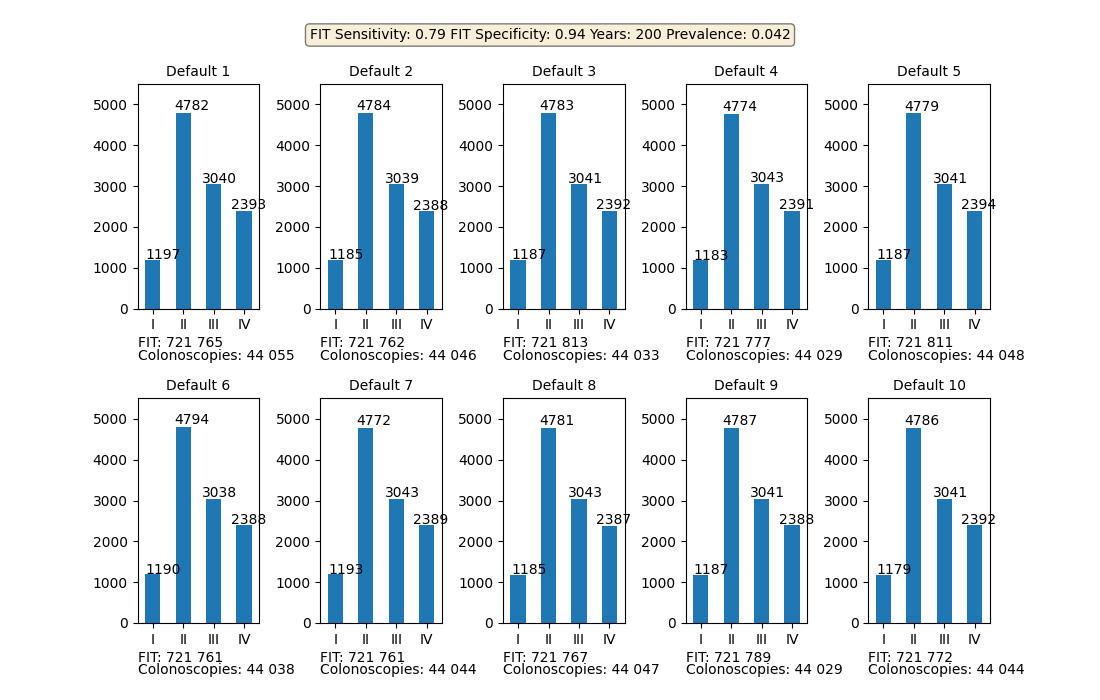
\includegraphics[width=1\textwidth]{images/5.results/treatments_for_defaults.png}
    \caption{Treatments for Default Replicas}
    \label{fig:treatments_for_default_replicas}
\end{figure}

Figure \ref{fig:treatments_for_default_replicas} illustrates that there are no notable changes in CRC stage distributions, and the number of FIT and colonoscopy procedures remains consistent across all scenarios.

\begin{figure}[H]
    \centering
    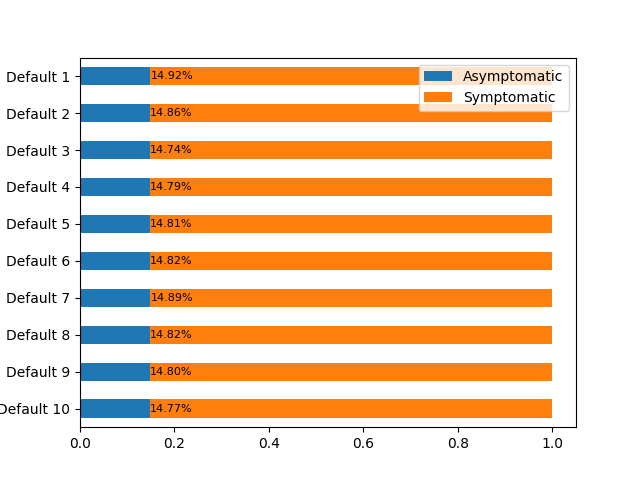
\includegraphics[width=1\textwidth]{images/5.results/screening_efficacy_for_defaults.png}
    \caption{Screening Efficacy for Default Replicas}
    \label{fig:screening_efficacy_for_default_replicas}
\end{figure}

In Figure \ref{fig:screening_efficacy_for_default_replicas}, the screening efficacy shows minor variations, with the most significant difference observed between scenarios amounting to a 0.18\% difference.

\begin{figure}[H]
    \centering
    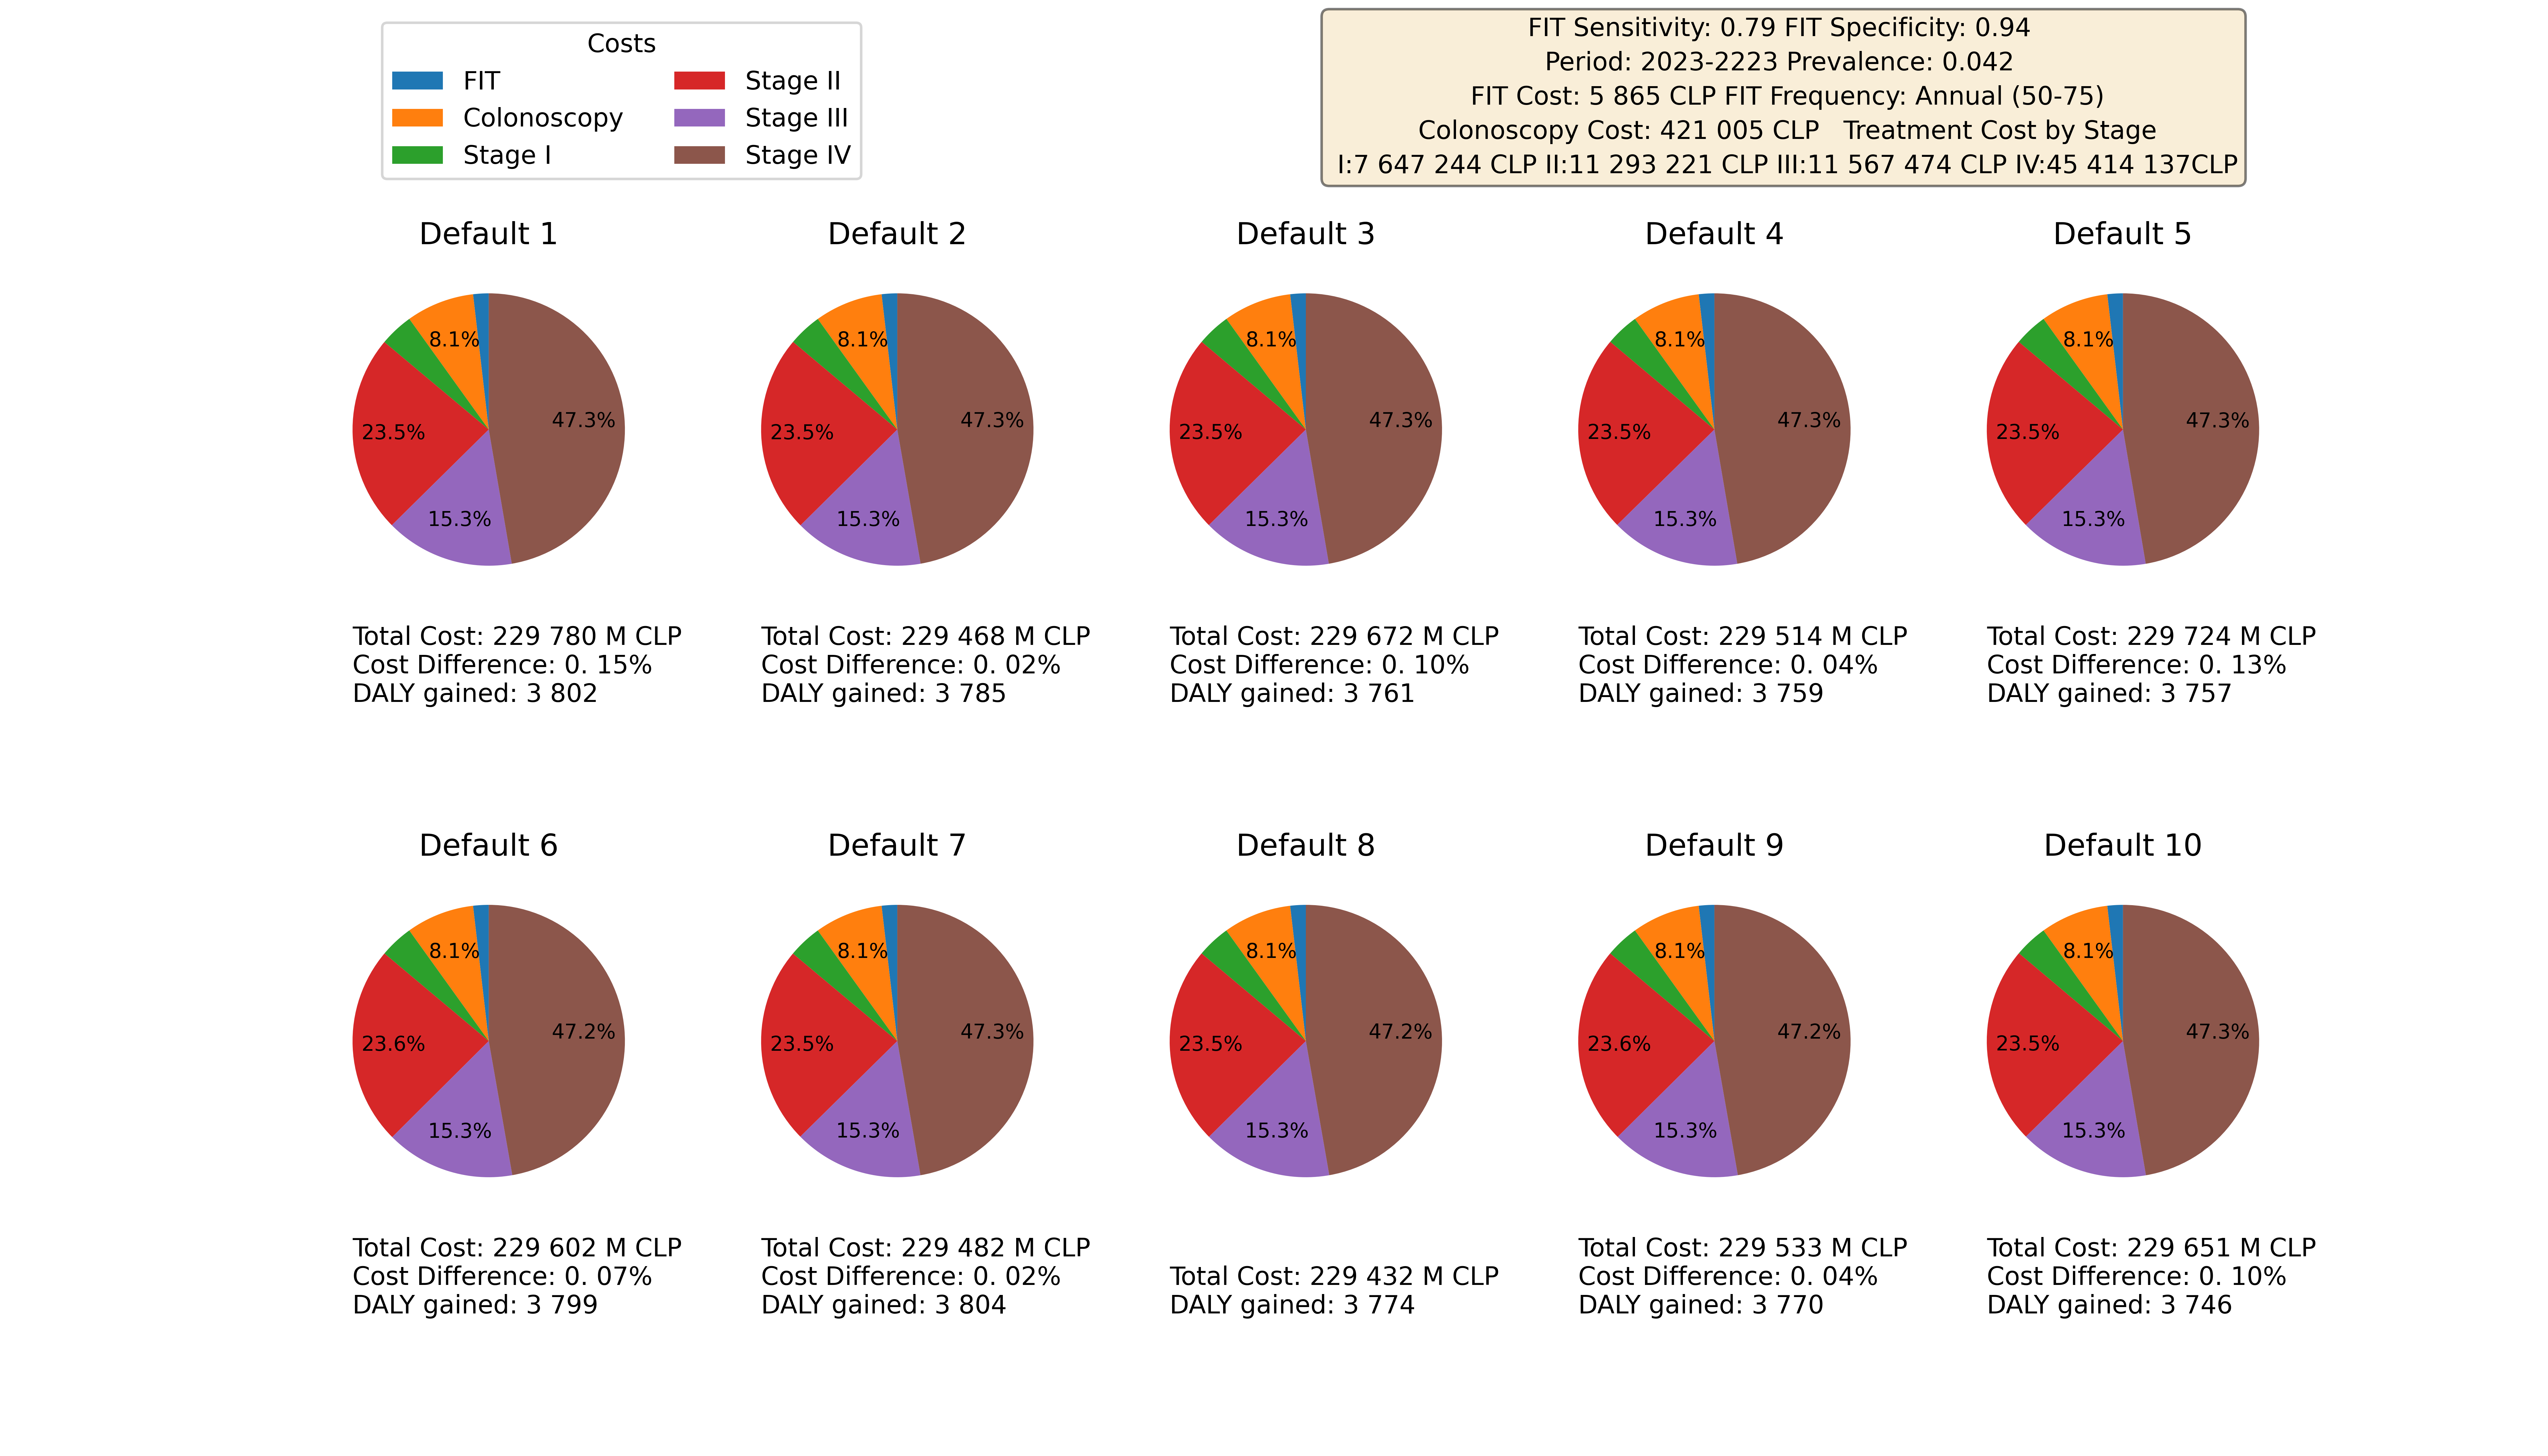
\includegraphics[width=1\textwidth]{images/5.results/costs_for_defaults.png}
    \caption{Costs for Default Replicas}
    \label{fig:costs_for_default_replicas}
\end{figure}

Figure \ref{fig:costs_for_default_replicas} depicts a consistent cost ratio across all scenarios. 'Default 8' is considered the baseline cost, being the lowest among all scenarios. The largest total cost difference between scenarios amounts to less than 0.2\%.

In conclusion, the replicas do not significantly impact this simulation model, as the variation between scenarios with the same parameters is negligible.

\section{Sensitivity Analysis: Screening Frequency}

In the simulation, we chose a biennial screening interval for FIT exams based on advice from a medical advisor. However, it's crucial to explore the effects of different screening frequencies to develop the best screening policy. This analysis aims to understand how the screening strategy's effectiveness is impacted by less or more frequent screenings. It's important to mention that these simulations spanned 200 years to reduce noise from the initial year and the adherence rate was set at 80\% for all scenarios.

\begin{figure}[H]
    \centering
    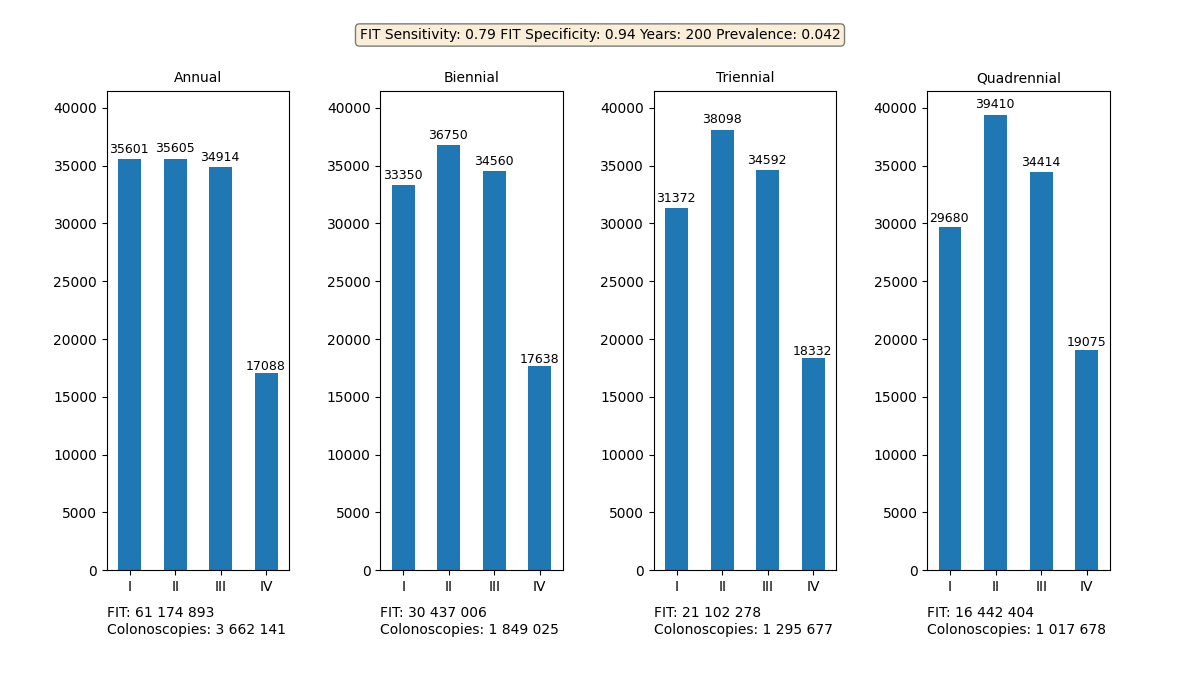
\includegraphics[width=1\textwidth]{images/5.results/treatments_by_frequency.png}
    \caption{Treatments by Screening Frequency}
    \label{fig:treatments_by_frequency}
\end{figure}

Figure \ref{fig:treatments_by_frequency} illustrates a significant decrease in the number of FIT and colonoscopy exams as the screening intervals increase. Moving from an annual to a biennial strategy notably reduces the number of exams conducted by half, and this reduction continues as the screening interval extends further to triennial and beyond.

\begin{figure}[H]
    \centering
    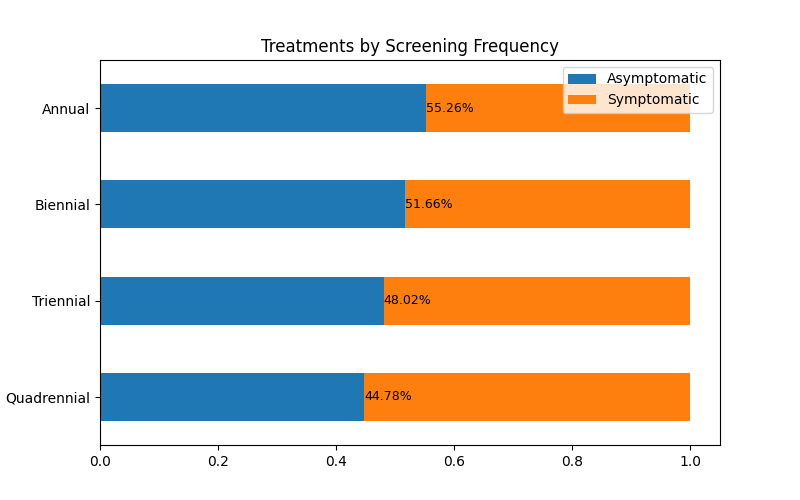
\includegraphics[width=1\textwidth]{images/5.results/screening_efficacy_by_frequency.png}
    \caption{Screening Efficacy by Frequency}
    \label{fig:screening_efficacy_by_frequency}
\end{figure}

Analyzing Figure \ref{fig:screening_efficacy_by_frequency}, transitioning from an annual to a biennial strategy reduces the number of exams, but there's a noticeable drop in performance of approximately 3\% each time the frequency is reduced.

\begin{figure}[H]
    \centering
    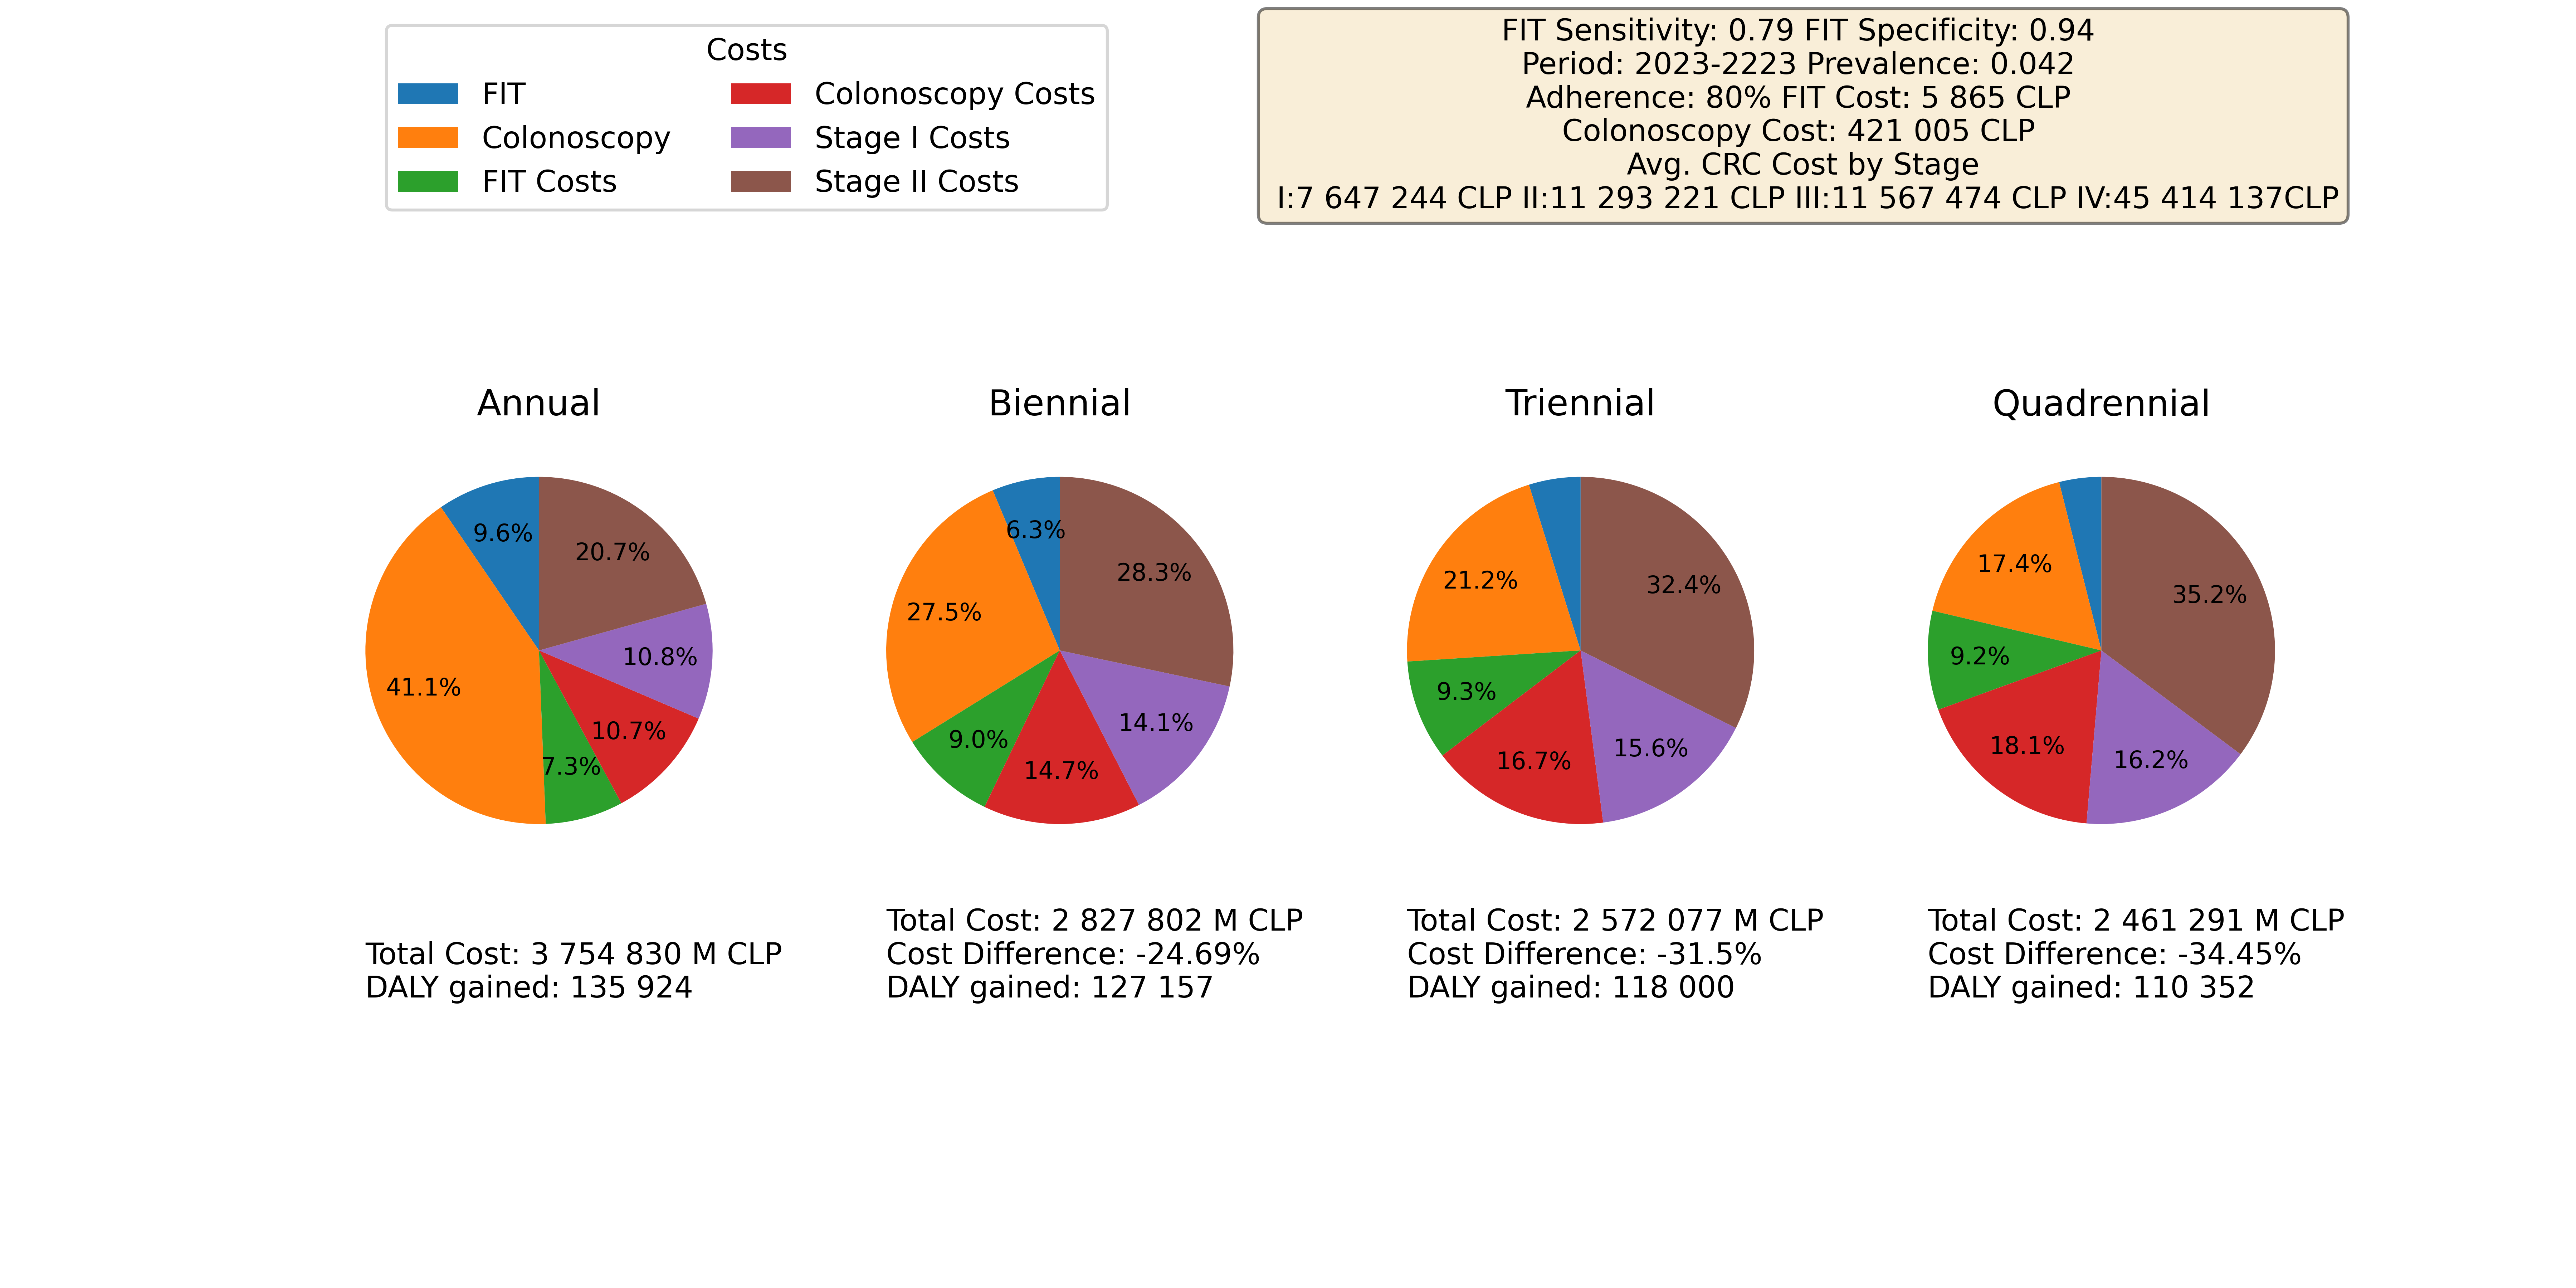
\includegraphics[width=1\textwidth]{images/5.results/costs_frequency.png}
    \caption{Costs by Frequency}
    \label{fig:costs_by_frequency}
\end{figure}

Now with Figure \ref{fig:costs_by_frequency} we can see that going from the annual strategy to the biennial strategy has a huge impact on the total costs of the system, reducing the costs by 25\%. Going from annual to triennial reduces the costs by 31\% so the reduction, even though it’s big, is not that significant.

In determining this parameter, an oncologist was consulted, providing insights into the optimal screening frequency. After reviewing the simulation's performances and associated costs, she concluded that while the cost reduction with a triennial screening was considerable, the corresponding performance metrics were not sufficiently robust. She cautioned against adopting a triennial screening interval, deeming it imprudent and advocating instead for a biennial screening strategy.

\section{Sensitivity Analysis: Screening Interval}

Currently, the screening interval spans from ages 50 to 75, encompassing a duration of 25 years for each individual. This timeframe aligns with the conventions observed in numerous European screening programs, which commonly adopt either this interval or the narrower range of 50 to 70 years. However, given the evolving landscape of life expectancy, alternative screening intervals warrant exploration to ascertain potentially superior outcomes. It's imperative to highlight that, to mitigate initial variability, the simulations were conducted over a 200-year span rather than the typical 20.

\begin{table}[H]
\caption{Simulations with different Screening Intervals}
\centering
\begin{tabular}{|c|c|c|c|}
\hline
Interval (years) & Total Cost M CLP & DALYs Gained & Efficacy Ratio\\ \hline
60-75 (15) & 2 600 602 (-8.4\%) & 82 086 (-35.4\%) & -4.21 \\ \hline
\rowcolor{lightred}
50-70 (20) & 2 748 535 (-3.2\%) & 113 373 (-10.8\%) & -3.39 \\ \hline
\rowcolor{lightred}
55-75 (20) & 2 735 710 (-3.7\%) & 107 962 (-15.1\%) & -4.13 \\ \hline
\textbf{50-75 (25)} & \textbf{2 839 398} & \textbf{127 150} &  \\ \hline
55-80 (25) & 2 826 202 (-0.5\%) & 116 735 (-8.2\%) & -17.62 \\ \hline
\rowcolor{lightgreen}
50-80 (30) & 2 976 125 (4.8\%) & 138 731 (9.1\%) & 1.89 \\ \hline
\rowcolor{lightgreen}
45-75 (30) & 2 996 982 (5.6\%) & 146 940 (15.5\%) & 2.8 \\ \hline
45-80 (35) & 3 082 601 (8.6\%) & 155 116 (22\%) & 2.57 \\ \hline
40-85 (45) & 3 362 547 (18.4\%) & 168 578 (32.6\%) & 1.77 \\ \hline
35-90 (55) & 3 595 708 (26.6\%) & 175 725 (38.2\%) & 1.43 \\ \hline
\end{tabular}
\subcaption*{The percentages are the differences between that simulation and the one with the \textbf{default parameters}. The Efficacy Ratio is the DALYs Gained Percentage divided by the Total Cost Percentage}
\label{table:simulation_intervals}
\end{table}

Table \ref{table:simulation_intervals} presents various options for selecting a new screening interval, each with its own cost and population impact considerations. Despite its apparent simplicity, this data provides valuable insights for budget adjustments.

For instance, if the goal is to expand the budget (highlighted in light green), lowering the starting age to 45 (45-75) yield better results in terms of DALYs gained per dollar spent than raising the upper age limit from 75 to 80 (50-80).

In contrast, if the aim is to reduce the budget (highlighted in light red), reducing the upper age limit from 75 to 70 (50-70) is more effective than increasing the starting age from 50 to 55 (55-75). While both approaches reduce the total costs, the 55 to 75 year interval produces a higher reduction in DALYs gained.

\section{Sensitivity Analysis: Colonoscopy Costs}

Conducting a sensitivity analysis on cost parameters is a standard practice in evaluating simulation models. This analysis allows us to understand how changes in cost parameters impact the feasibility of the proposed project. In Figure \ref{fig:costs_by_adherence}, we observe that at 80\% adherence, colonoscopy costs account for about 29\% of the total. However, the precise cost of a colonoscopy remains unclear due to significant variations in the obtained prices. Therefore, a sensitivity analysis on colonoscopy costs is called for.

The baseline parameter, which is the average cost across three clinics, provides a reference point for comparison. By individually assessing the influence of each clinic's cost on the simulation outcomes, we can examine how variations in this crucial parameter affect the overall results.

\begin{figure}[H]
    \centering
    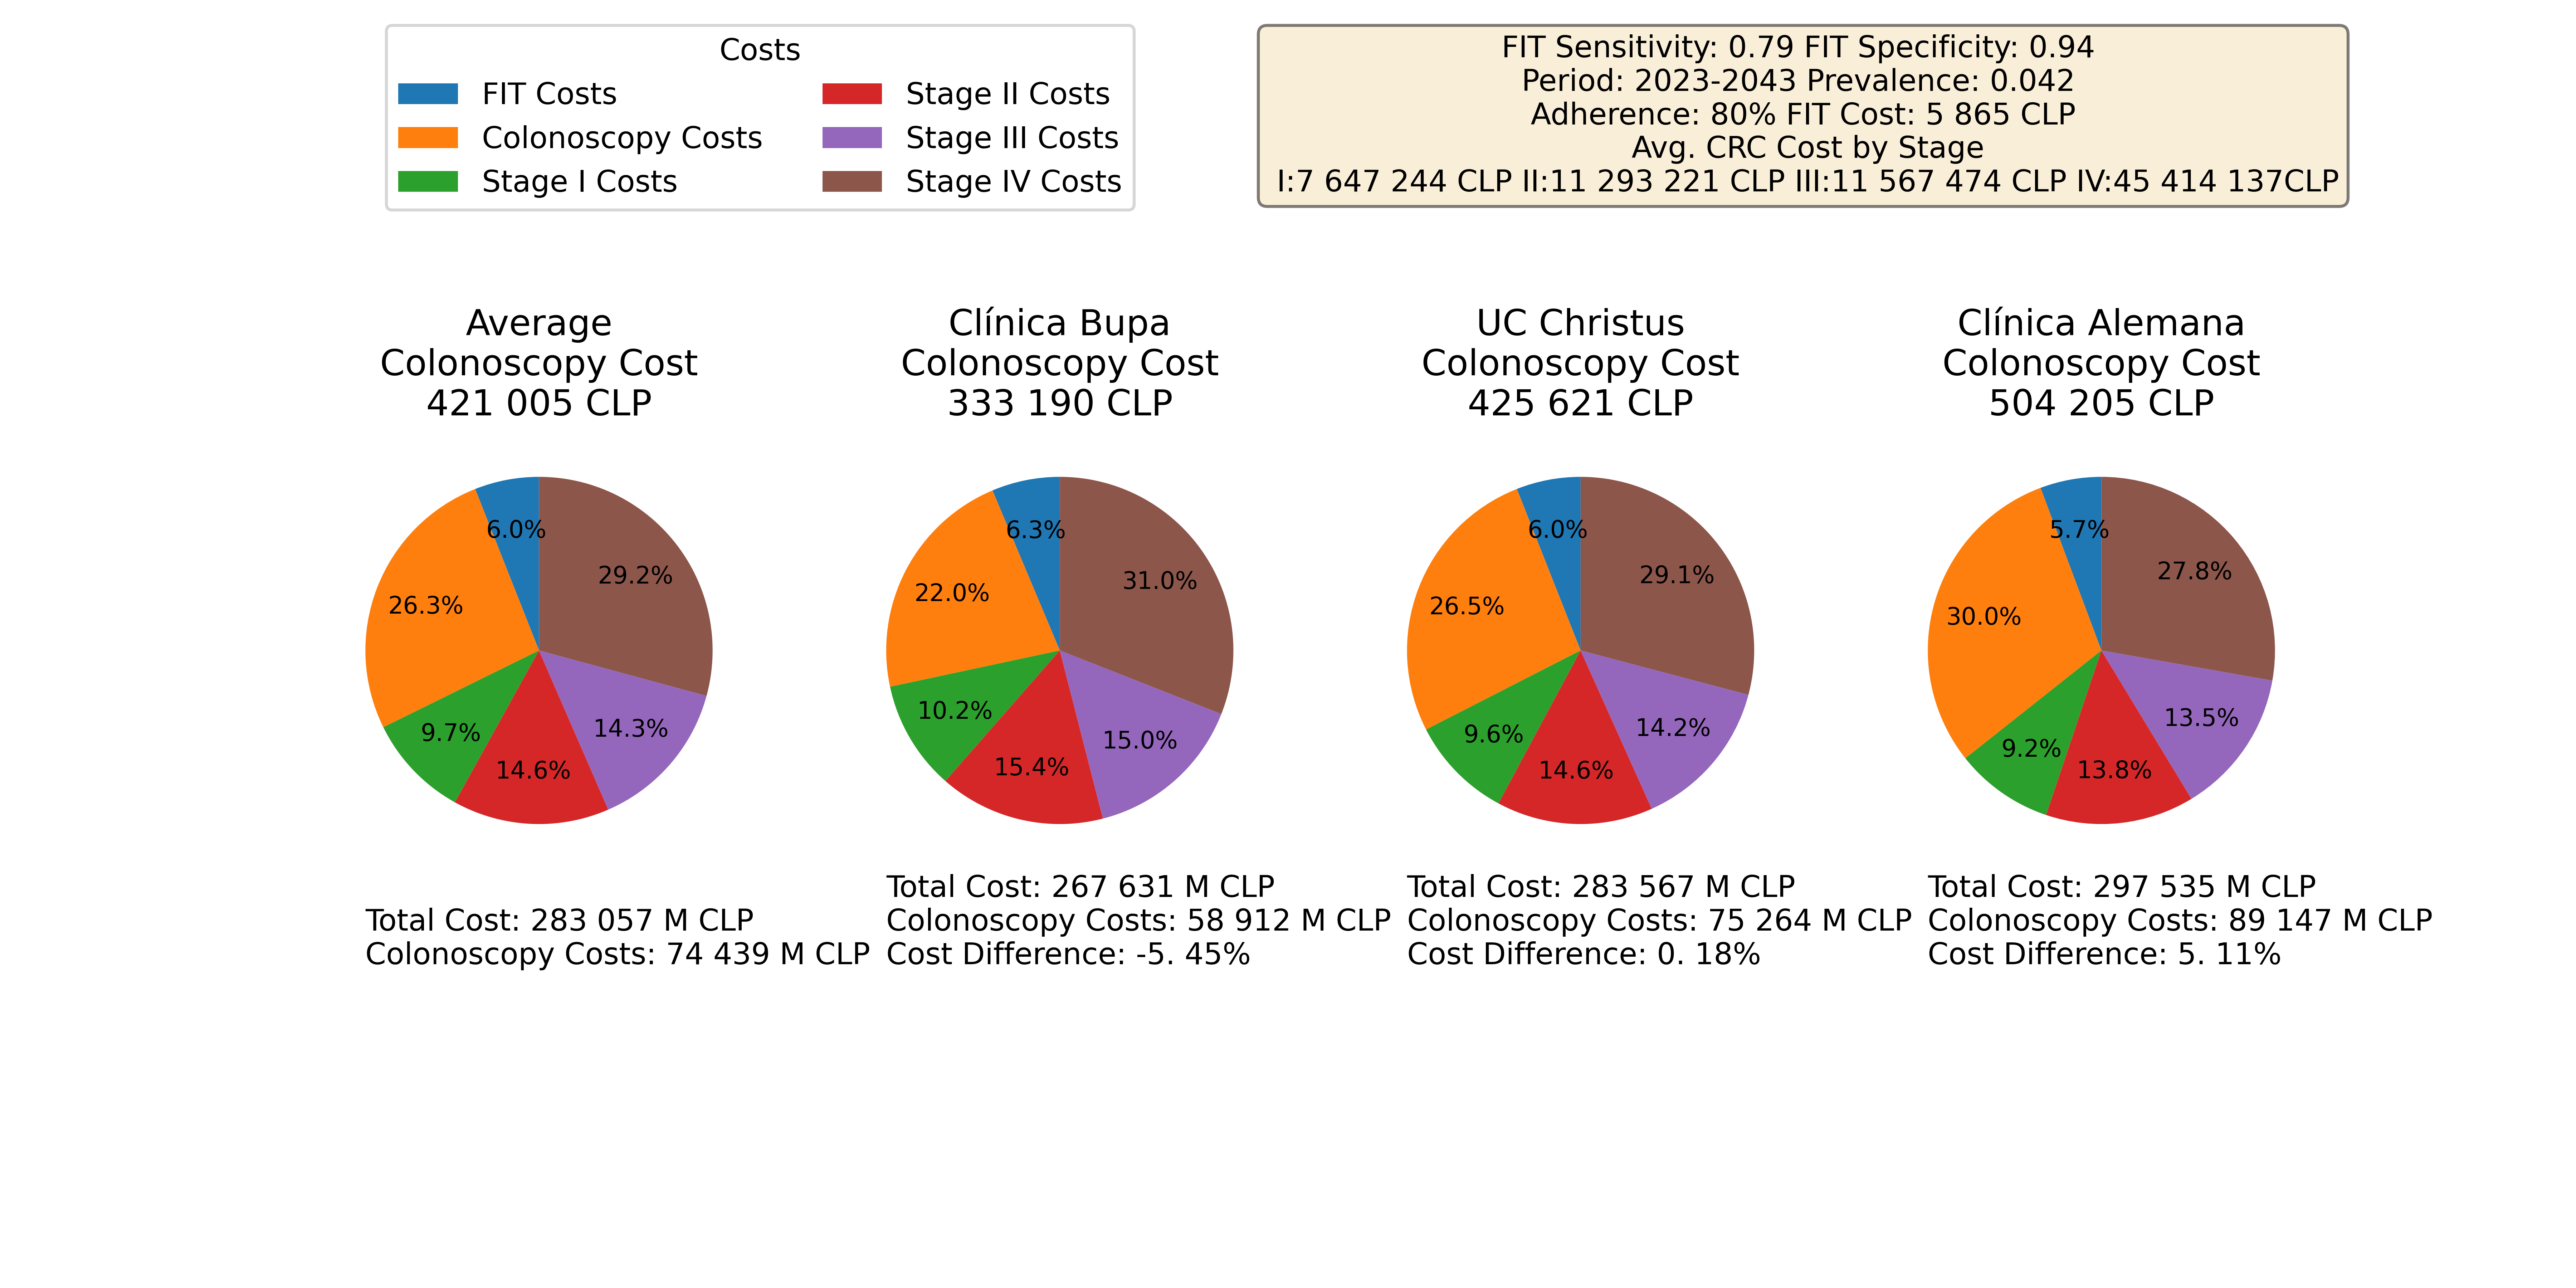
\includegraphics[width=1\textwidth]{images/5.results/costs_colonoscopies.png}
    \caption{Colonoscopy Costs}
    \label{fig:colonoscopy_costs}
\end{figure}

The charts in Figure \ref{fig:colonoscopy_costs} takes a look at how the colonoscopy exams affect the overall costs for screening colorectal cancer. It's clear that the cost of colonoscopy exams is an important part of managing the budget for colorectal cancer treatments as the lower and upper bound of total costs differentiate about 5\% from the average.

\section{Sensitivity Analysis: FIT Performance Indicators}

\subsection*{Improved Sensitivity}

The enhancement in sensitivity is expected to have a straightforward effect on the simulation. As the detection of patients with the disease improves or worsens, the percentage of asymptomatic detection should correspondingly improve or deteriorate. This adjustment is unlikely to significantly impact costs, as the main effect lies in potential shifts of treatments to earlier stages.

\begin{figure}[H]
    \centering
    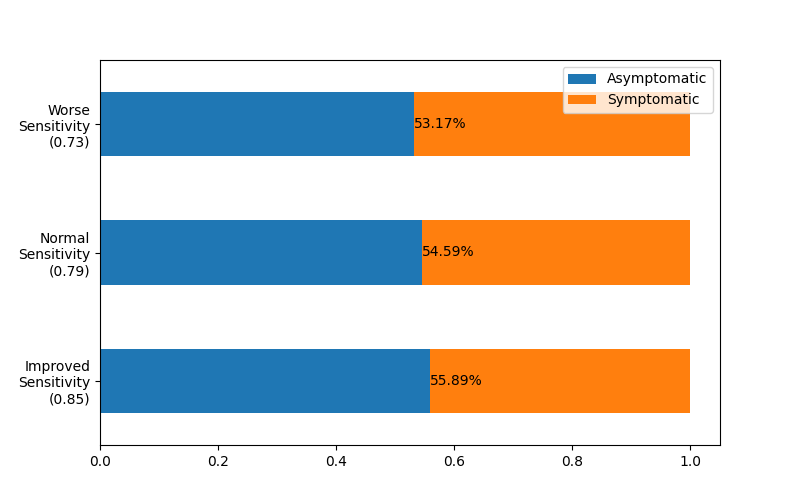
\includegraphics[width=1\textwidth]{images/5.results/screening_efficacy_by_fit_sensitivity.png}
    \caption{Screening Efficacy by FIT Sensitivity}
    \label{fig:screening_efficacy_by_sensitivity}
\end{figure}

In Figure \ref{fig:screening_efficacy_by_sensitivity} is observed that for every 6\% change in sensitivity, there's approximately a 1\% decrease or increase in asymptomatic detection. The impact on costs was minimal, representing around 0.1\% of the total cost.

\subsection*{Improved Specificity}

The improvement in specificity is expected to have a direct impact on the simulation costs. As the detection of patients without the disease improves or worsens, the number of false positives should accordingly decrease or increase. Since false positives require a colonoscopy, reducing their number results in an overall decrease in the cost of the entire system. Additionally, a scenario of almost perfect specificity was included to test the upper bound of this effect on the simulation.

\begin{figure}[H]
    \centering
    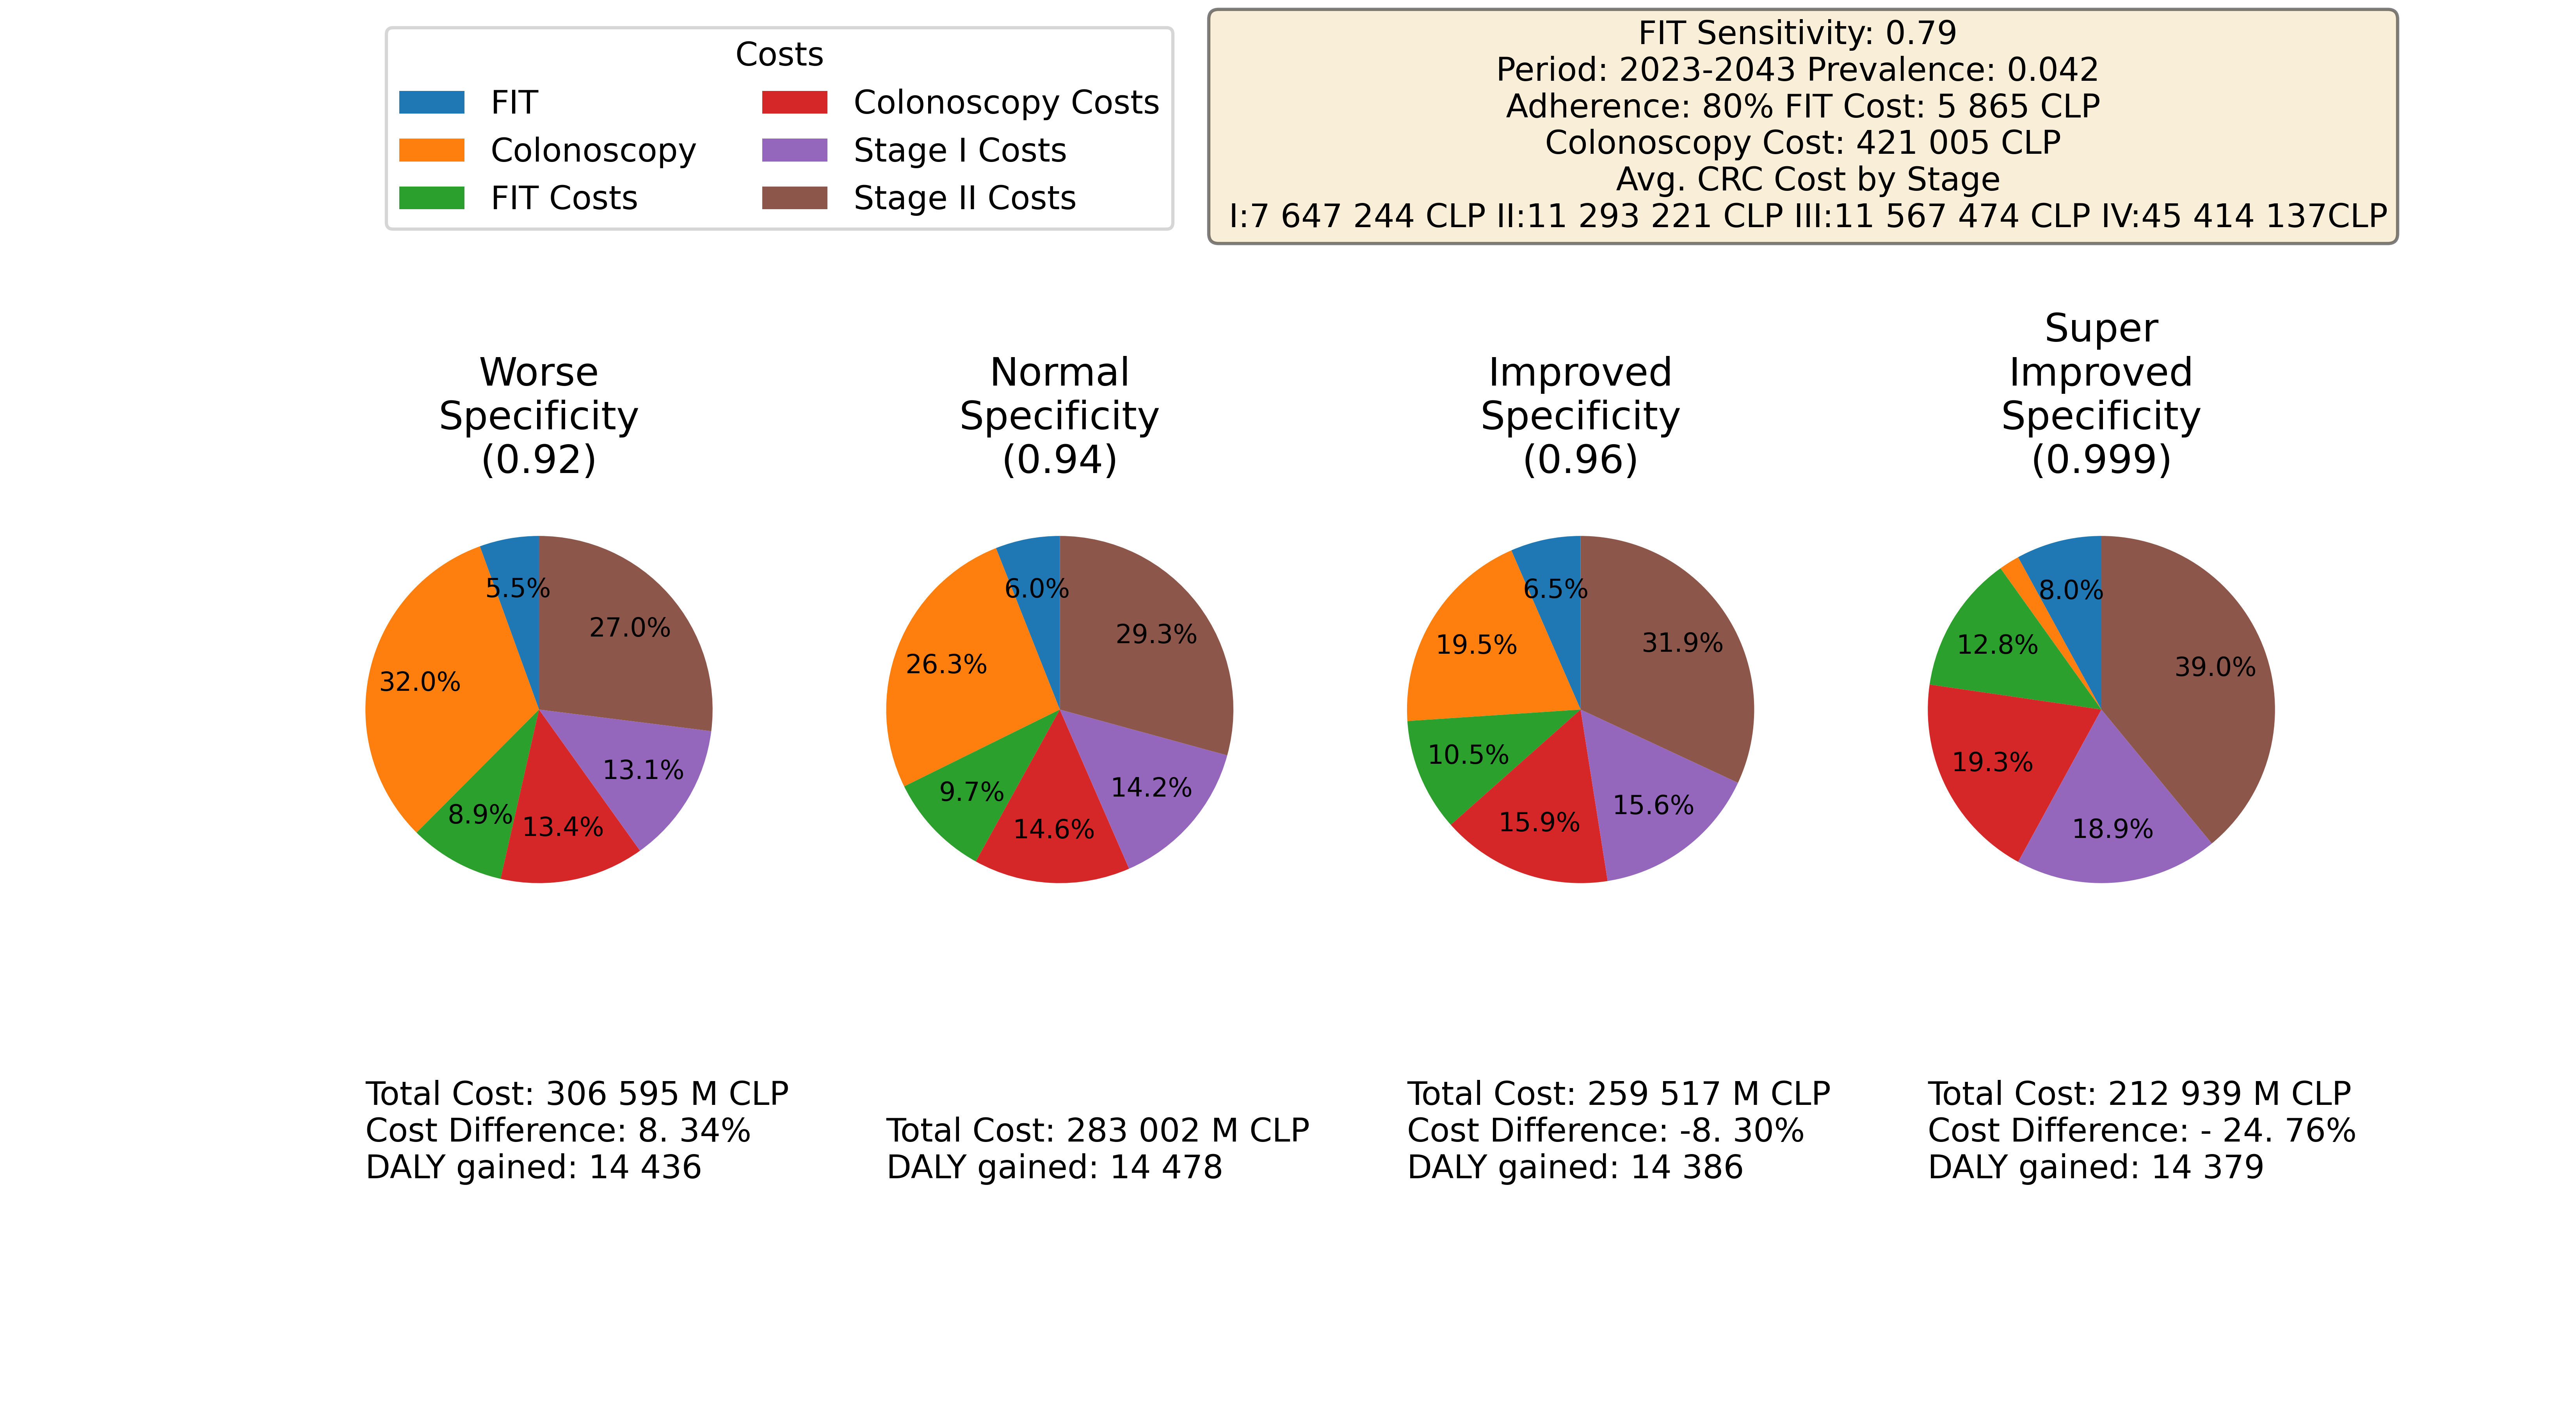
\includegraphics[width=1\textwidth]{images/5.results/costs_fit_specificity.png}
    \caption{Costs by FIT Specificity}
    \label{fig:costs_by_specificity}
\end{figure}

Figure \ref{fig:costs_by_specificity} illustrates the significant impact of improving or worsening the FIT specificity on the overall cost of the system. Even minor changes in specificity, such as a 2\% improvement or worsening, result in approximately a 8\% shift in the overall cost, highlighting its notable significance. When pushed to nearly perfect specificity, the screening strategy becomes cost-effective as the total cost is less than the 0\% adherence scenario in Figure \ref{fig:costs_by_adherence}.


\chapter[Conlusions and Discussion]{Conlussions and Discussion} 
\label{chapter:conclusions}
The objective of this thesis was to investigate and analyze the colorectal cancer (CRC) care process within the SMPHS, proposing improvements to enhance patient prognosis. This chapter focuses on presenting the main results of the study, discussing its methodology and value, assessing the accomplishment of its objectives, and providing recommendations for related fields.

\section{Main Findings}

\subsection*{Process Discovery}
The process discovery phase aimed to understand the functioning and performance of the CRC care process, with a focus on the key stages of diagnosis and treatment. Initially, the primary goal seemed to be the opportune delivery of treatment. However, as the study progressed, it became clear that preventive medicine could significantly improve prognosis and reduce costs, despite the need for substantial effort and resources to design a CRC screening strategy. This shift in focus led to an emphasis on improving disease prognosis as the new goal of the CRC care process.

The data analysis revealed that the current system is failing to provide opportune diagnosis and treatment to patients. This is likely to cause discomfort and mistrust among patients using the public healthcare system, potentially leading many of them to abandon treatment.

\subsection*{Process Improvement}

It was determined that the process improvement would be designing a screening strategy and validating it with a microsimulation model. While this approach does not resolve all the identified issues in CRC care, it means an improvement in patient prognosis, which is the primary objective.

The program was inspired by previous CRC screening models and aimes to utilize state-of-the-art knowledge about the disease and the SMPHS population. After completion, the model showed promising results for improving patient prognosis. However, it also indicated that this enhancement comes with increased overall costs. It is now up to the authorities to assess the feasibility and value of implementing the screening strategy.

\section{Discussion}

\subsection*{Challenges of the Study}

The MND team played a crucial role in supporting the data collection process. However, the absence of a standardized procedure for accessing government data for research purposes complicated this stage. Despite clear collaboration intentions from the SMPHS, obtaining the data was not as immediate as hoped.

The primary data source, the SIGGES system, provided reasonably clean data for analysis but lacked the level of quality and detail required for reviewing complex cases. Additionally, the uncertainty surrounding the data made it challenging to distinguish between complex cases and data noise, leading to the exclusion of these cases from the analysis.

Furthermore, in the beginning, there was no established methodology for Process Mining in the process discovery phase. Therefore, the researcher spent a considerable amount of time discovering most preprocessing techniques on its own. Discovering the MEDCP methodology later provided reassurance that the prior work was correct but highlighted the unnecessary time lost.

One of the most challenging decisions in this project was whether to utilize an existing simulation model or to develop one from scratch. Despite efforts to obtain other simulation models' code for reference or to gather insights not available in their published papers, these attempts were unsuccessful. This made the researcher hesitant before deciding to proceed with developing the model independently.

Another ongoing challenge is the lack of specific medical information about CRC in Chile. The characteristics of the disease, such as prevalence and sojourn times for each stage, can vary significantly between regions. For the microsimulation, having more detailed medical data from the simulated region would have greatly enhanced the reliability of the outcomes.

\subsection*{How can we improve in the Future?}

The data collection process did not have a clear mistake by the researcher, aside from the approach of attempting to gather all data from a single source. A missed opportunity was not exploring additional data sources, such as private clinics, which routinely collect data on this disease.

The overlooking of complex cases could have been mitigated in two ways. Firstly, with a larger and higher-quality dataset, the researcher could have identified more complex cases and potentially uncovered explanations for these instances. Secondly, with additional medical expertise, the researcher would have had more support in understanding the complexities and nuances of the more intricate cases.

Understanding how to preprocess the available data was challenging due to the lack of a clear methodology. And the MEDCP methodology provided clear guidance on the necessary preprocessing techniques for this type of project. It is recommended for future projects to allocate dedicated time and resources to finding a suitable methodology for achieving the desired objectives.

In retrospect, the process of obtaining other simulation models should have been initiated earlier. A key mistake was not starting this phase of the thesis sooner and not being decisive enough on when to start the project from scratch. Starting this phase earlier would have increased the likelihood of obtaining access to a functional simulation model or its code. Additionally, being more decisive about starting the simulation model could have allowed for more time to its development and validation.

Regarding the lack of medical information of CRC from Chile, the researcher has exhausted all available public data sources. To address this challenge, the simulation's code repository has been made public, allowing for future improvements and updates as new medical data becomes available.

\section{Value and Replicability of this Study}

The discovery, analysis, and improvement strategy of the CRC care process are highly valuable for various stakeholders.

For the SMPHS and other healthcare institutions managing CRC, this study provides a comprehensive analysis of the CRC care process, offering valuable insights for future improvement decisions. While the focus is on CRC care in this specific region, similar analyses could be conducted for other diseases covered by the Explicit Guarantees in Health (GES) program or in different regions of the country with minor adjustments.

Regarding Process Mining, the use of the MEDCP methodology adds credibility to the results and demonstrates its effectiveness in conducting projects related to diseases like CRC. This study adds to the growing body of work that uses Process Mining to identify common disease pathways and provide key insights into care process performance.

Finally, the simulation model shows promise in improving patient prognosis. While further validation by external validators is necessary to establish its credibility, the model successfully achieves its goal of creating a valid screening simulation model. Additionally, the use of microsimulation for this particular case proves highly useful in assessing the feasibility and cost-effectiveness of implementing this public policy project.

\section{Conclusions}

The project of understanding and analysing the CRC care process through raw data was succesful, as it allowed the researcher to propose valid advice to the SMPHS on how to improve. The results of the process discovery and analysis were supported by real-data analysis and performance indicators that identified genuine issues the service is facing.

The microsimulation model produced in this study met the desired objectives. The data used was obtained from reliable sources, and the outcomes were consistent with various screening strategies worldwide.  Furthermore, the use of sensitivity analyses on key parameters further strengthened the reliability of the findings. The results confirm an improvement in prognosis with increased population participation in the screening program. While the overall costs of implementing these procedures rise, it is the responsibility of the authorities to evaluate the cost-effectiveness of this project and decide whether to proceed with its implementation.

\section{Further Work}

\subsection*{SIGGES Data Collection and Accesibility}

As previously mentioned, the researcher appreciates the government's efforts to track the diagnosis and treatment of each GES disease. However, this study uncovered indications of potential issues with the data and its collection process. While access to the data was eventually granted, the process was clumsy and time-consuming. If the government aims to promote healthcare system improvements, streamlining the process for accessing anonymized datasets would facilitate research endeavors and contribute to a better understanding of healthcare dynamics.

\subsection*{CRC Microsimulation Model}

The researcher concludes that the simulation developed for this study is well-suited to the available data, given the constraints of time and resources inherent in a master's thesis project. The simulation adequately captures key aspects of the CRC care process, offering valuable insights and informing recommendations for further research and policy development.

The model utilized in this study will be accessible in a public repository, enabling anyone interested to test, critique, or enhance it. The researcher hopes for ongoing development and refinement of this simulation model, welcoming contributions from the broader community to further improve its accuracy and effectiveness.

\subsection*{Replication for other diseases}

The main recommendation from this study is to conduct similar analyses for all diseases within the Chilean public healthcare system. By examining successful implementations of new strategies in other countries, many of these approaches can be evaluated for their feasibility and cost-effectiveness.

While the focus of this study is on colorectal cancer, its findings highlight the wider potential for preventive measures across the range of the 94 diseases covered under the GES system. It is hoped that each of these conditions will undergo thorough analysis for the possible integration of preventive medicine, with the ultimate goal of enhancing public health outcomes nationwide.



%%%%%%%%%%%%%
%       REFERENCES        %
%%%%%%%%%%%%%

\cleardoublepage
\phantomsection \label{references}
\bibliographystyle{apacite}
\renewcommand{\bibname}{REFERENCES}

%%%% ACTIVAR SIGUIENTES 3 LINEAS SI POSTGRADO RECHAZA LA BIBLIOGRAFIA
\setlength{\bibleftmargin}{0em}
\setlength{\bibindent}{0em}
\setlength{\bibitemsep}{1em}

\bibliography{Thesis}
\end{document}
